% mn2esample.tex
%
% v2.1 released 22nd May 2002 (G. Hutton)
%
% The mnsample.tex file has been amended to highlight
% the proper use of LaTeX2e code with the class file
% and using natbib cross-referencing. These changes
% do not reflect the original paper by A. V. Raveendran.
%
% Previous versions of this sample document were
% compatible with the LaTeX 2.09 style file mn.sty
% v1.2 released 5th September 1994 (M. Reed)
% v1.1 released 18th July 1994
% v1.0 released 28th January 1994

\documentclass[useAMS,usenatbib]{mn2e}

% If your system does not have the AMS fonts version 2.0 installed, then
% remove the useAMS option.
%
% useAMS allows you to obtain upright Greek characters.
% e.g. \umu, \upi etc.  See the section on "Upright Greek characters" in
% this guide for further information.
%
% If you are using AMS 2.0 fonts, bold math letters/symbols are available
% at a larger range of sizes for NFSS release 1 and 2 (using \boldmath or
% preferably \bmath).
%
% The usenatbib command allows the use of Patrick Daly's natbib.sty for
% cross-referencing.
%
% If you wish to typeset the paper in Times font (if you do not have the
% PostScript Type 1 Computer Modern fonts you will need to do this to get
% smoother fonts in a PDF file) then uncomment the next line
% \usepackage{Times}
 \usepackage{times}

%%%%% AUTHORS - PLACE YOUR OWN MACROS HERE %%%%%

\usepackage{graphicx}
\usepackage{supertabular}
\usepackage{subfig}
\usepackage{rotating}
\usepackage{lscape}
\usepackage{epsfig}
%\usepackage{natbib}
\usepackage{amssymb}
%\usepackage{myaasmacros}
\usepackage{amsmath}
\usepackage{multicol}
%\usepackage{makecell}
%\usepackage{slashbox}
\usepackage{color}
\usepackage{tikz}

\bibliographystyle{astron}

\def\squig{$\sim\!\!$}
\def\lesssim{\mathrel{\hbox{\rlap{\hbox{\lower4pt\hbox{$\sim$}}}\hbox{$<$}}}}
\def\gtrsim{\mathrel{\hbox{\rlap{\hbox{\lower4pt\hbox{$\sim$}}}\hbox{$>$}}}}
\def\subsun{\mbox{$_{\normalsize\odot}$}}
\def\arcsec{\hbox{$^{\prime\prime}$}}
\def\arcmin{$^{\prime}$}
\def\deg{\hbox{$^\circ$}}
\def\mic{ $\mu $m\,}
%\def\power{WHz$^{-1}$sr$^{-1}$}
%\def\flux{erg s$^{-1}$ cm$^{-2}$}
%\def\lum{erg s$^{-1}$}
%\def\14{\rm 1.4\,GHz}
%\def\27{\rm 2.7\,GHz}
%\def\whz1{$\,\rm W\,Hz^{-1}$}
%\def\kms1{$\,\rm km\,s^{-1}$}

\def\aas{A\&A Sup} 
\def\apj{ApJ} 
\def\apjs{ApJSup} 
\def\mnras{MNRAS} 
\def\aaps{AAPS}
\def\pasp{PASP} 
 

%%%%%%%%%%%%%%%%%%%%%%%%%%%%%%%%%%%%%%%%%%%%%%%%

\title[The Herschel--ATLAS 2nd data release]{HATLAS-DR2}
\author[S.J. Maddox]{\parbox{\textwidth}{S.J. Maddox$^{1}$
\thanks{E-mail: maddoxs@cardiff.ac.uk}, et al }}

\begin{document}

\date{}

\pagerange{\pageref{firstpage}--\pageref{lastpage}}\pubyear{2016}

\maketitle

\label{firstpage}

\begin{abstract}
  We present the second public release of source catalogues from the
  Herschel-ATLAS survey. The catalogued area in this release covers a
  total of 480 square degrees: 177 square degrees in the north
  galactic cap, and 303 square degrees in the southern galactic
  cap. The catalogues contain 114368 and 183784 sources detected at
  more than 4 sigma significance in any of the 250\mic, 350\mic or
  500\mic bands band. The rms positional accuracy for the faintest
  sources is about 2.4 arc seconds in ra and dec. Photometry is
  presented for 5 Herschel bands: 100, 160, 250, 350 and 500\mic. We
  show the distribution of sources as a function of signal-to-noise,
  and as a function of flux.
  


\end{abstract}

\begin{keywords}

\end{keywords}

\section{Introduction}

The Herschel mission has revolutionized the study of the FIR sky. The
Herschel-ATLAS was the largest project awarded time in the open
allocations, and mapped 659 square degrees of sky.  The footprint of
the survey is spread between 5 disjoint areas: 3 equatorial fields
each covering ~50 square degrees, giving a total of 161 square
degrees; a roughly square region covering 180 square degrees centred
on the North Galactic Pole, see Fig~\ref{skymapn}; and an elongated
region covering 318 square degrees in the south galactic cap see
Fig~\ref{skymaps}.  The maps and source catalogues for the equatorial
fields were described by Valiente et al 2016 (hereafter V16).  The
creation of maps for the NGP and SGP areas is detailed in the
companion paper (Smith et al 2017; hereafter S17). In this paper we
describe source detection and catalogues for the NGP and SGP areas. We
detect sources and measure their fluxes in areas which are covered by
multiple scans by the Herschel detectors, and so the catalogued areas
cover 177 square degrees in the NGP, and 303 square degrees in the
SGP, slightly smaller than the full area covered by the maps. For the
NGP area, identifications to optical sources are presented in a second
companion paper (Furlanetto et al 2017; hereafter F17).

In this paper we describe the process followed to create the source
catalogues. In section 2 we describe the source detection process, and
our flux measurements; in Section 3 we present our estimates of the
flux uncertainties; in Section 4 we show the positional uncertainties;
Section 5 discusses the completeness and purity of the source
catalogue. The catalogue files of the release are described in the
Appendix.


\begin{figure} %1 
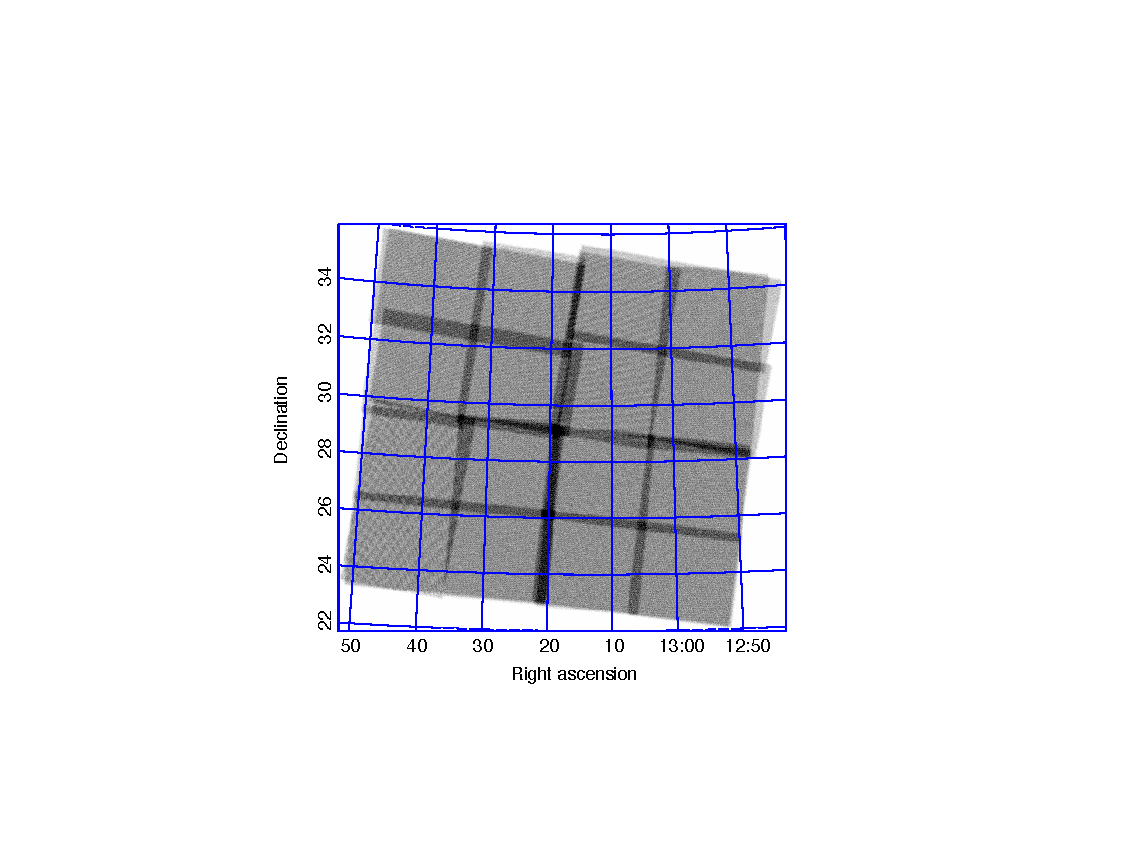
\includegraphics[scale=0.7]{ngpcoverage.pdf}
\caption{\protect\label{skymapn} The coverage map for 250\mic data
  in the North Galactic Pole area. The coverage varies from 1 to 43
  detector passes with the 5\%, median and 95\% values being 7, 10 and
  16 detector passes. The gray-scale goes from white, 0 passes, to
  black, 27 passes.}

\end{figure}

\begin{figure*} %2 
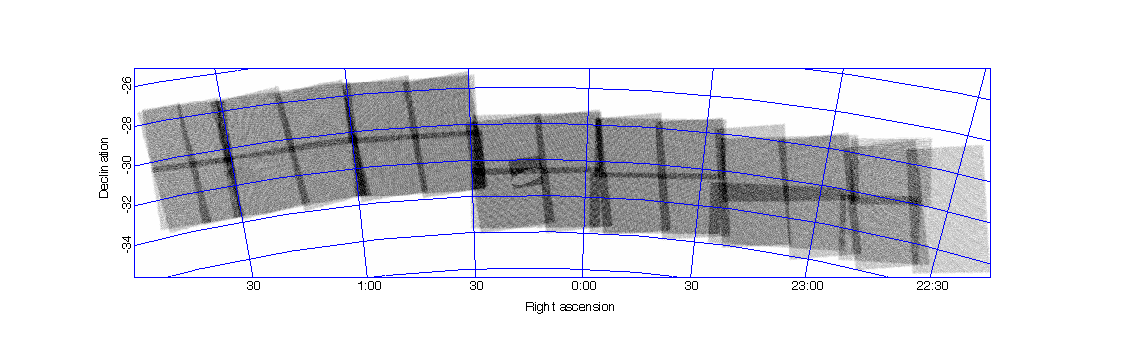
\includegraphics[scale=1.]{sgpcoverage.pdf}
\caption{ \protect\label{skymaps} The coverage map for 250\mic data
  the South Galactic Pole area.  The number of detector passes per
  pixel varies from 1 to 36, with the 5\%, median and 95\% values
  being 7, 9 and 14 detector passes with the median of 9 detector
  passes. In 1, 2, 3 and 4-scan regions the mean number of detector
  passes is 4.8, 9.6, 14.4 and 19.2. The gray-scale goes from white, 0
  passes to black, 21 passes.  }

\end{figure*}


 

\section{ Source detection and catalogues } 

\subsection{Maps and Background subtraction} 

A detailed description of the processing to produce maps from the
Herschel raw data is presented in S17. The resulting maps maps have
pixel sizes 3, 4, 6, 8 and 12 arc seconds for 100, 160, 250, 350 and
500 microns respectively. The PACS maps (100 and 160\mic) have units
of Jy per pixel. The SPIRE maps have units of Jy per beam and the beam
areas are 469, 831 and 1804 square arc seconds.


Before attempting to detect sources in the maps, we first subtract a
smoothly varying 'sky' level to remove the flux contributed by
foreground emission from dust in our galaxy, and also by the varying
background from clustered sources fainter than our detection limit. We
use the {\tt nebuliser} function from the CASU package to estimate and
subtract this background level (see
http://casu.ast.cam.ac.uk/surveys-projects/software-release/background-filtering). The
filter scales used in {\tt nebuliser} must be small enough to follow
relatively small-scale features in some patches of foreground cirrus,
but not so small that extended source fluxes are reduced.


For the SPIRE maps we found that a median filter scale of 30 pixels (3
arc minutes in the 250 \mic band) followed by a linear filter scale of
15 pixels was an acceptable combination. We tested this by creating
simulated maps with large sources and measuring the source fluxes
after applying nebuliser. The sources were given exponential profiles
truncated at 5 scale-lengths, and then convolved by the SPIRE point
spread function.  The truncation at 5 scale-lengths corresponds
roughly to an optical isophotal radius at $\mu_r ~ 25 $mag
arcsec$^{-2}$. The scale-lengths were varied so that the equivalent D25
diameters ranged from 12'' to 96''.
%% !!!
These simulations showed that significant flux is lost only for
sources that have diameters larger than $~3$ arc minutes, and even at
this size, the flux loss is $\lesssim 10\%$.

Since the extra-galactic background comes from the sum of clustered
distant galaxies, the local background level varies across the sky;
the nebuliser background estimate includes this variation, and so will
remove it along with foreground emission. Source catalogues made
without any background subtraction will include more sources where the
background is high from unresolved clusters, and so will have higher
apparent clustering than an unbiased flux-limited sample. 

For the PACS maps, $1/f$-noise from the instrument is much larger than
for SPIRE, so foreground emission is a less significant
contribution. This means that we can use a larger nebuliser scale, 5
arc minutes.

The resulting maps have a modal pixel value which is close to
zero. For the SPIRE bands, the instrumental noise is low enough that
flux distribution of detected sources skews the pixel distribution to
positive values so the mean is slightly positive (1.0, 1.0 and 0.6
mJy/beam at 250, 350 and 500 \mic).
The PACS detector is less sensitive and less stable than SPIRE, and so the
instrumental noise dominates over the confusion noise and the pixel
distribution is close to Gaussian; the mean of the {\tt nebulised} PACS
maps are very close to zero (0.009mJ/pixel, or 0.016 and 0.016
MJy/str respectively for the 100 and 160\mic maps). 

%NGP
%100.000000 0.009532 0.000000 
%160.000000 0.015944 0.000000 
%250.000000 0.986214 1.040600 
%350.000000 0.957390 0.844167 
%500.000000 0.622022 0.551361 

%sgp
%100.000000 0.008460 0.000000 
%160.000000 0.015806 0.000000 
%250.000000 0.931874 0.901568 
%350.000000 0.891035 0.780424 
%500.000000 0.587480 0.521348 

\subsection{Source Detection} 


\begin{figure} %3 
  %(a)\hspace{-1mm}
  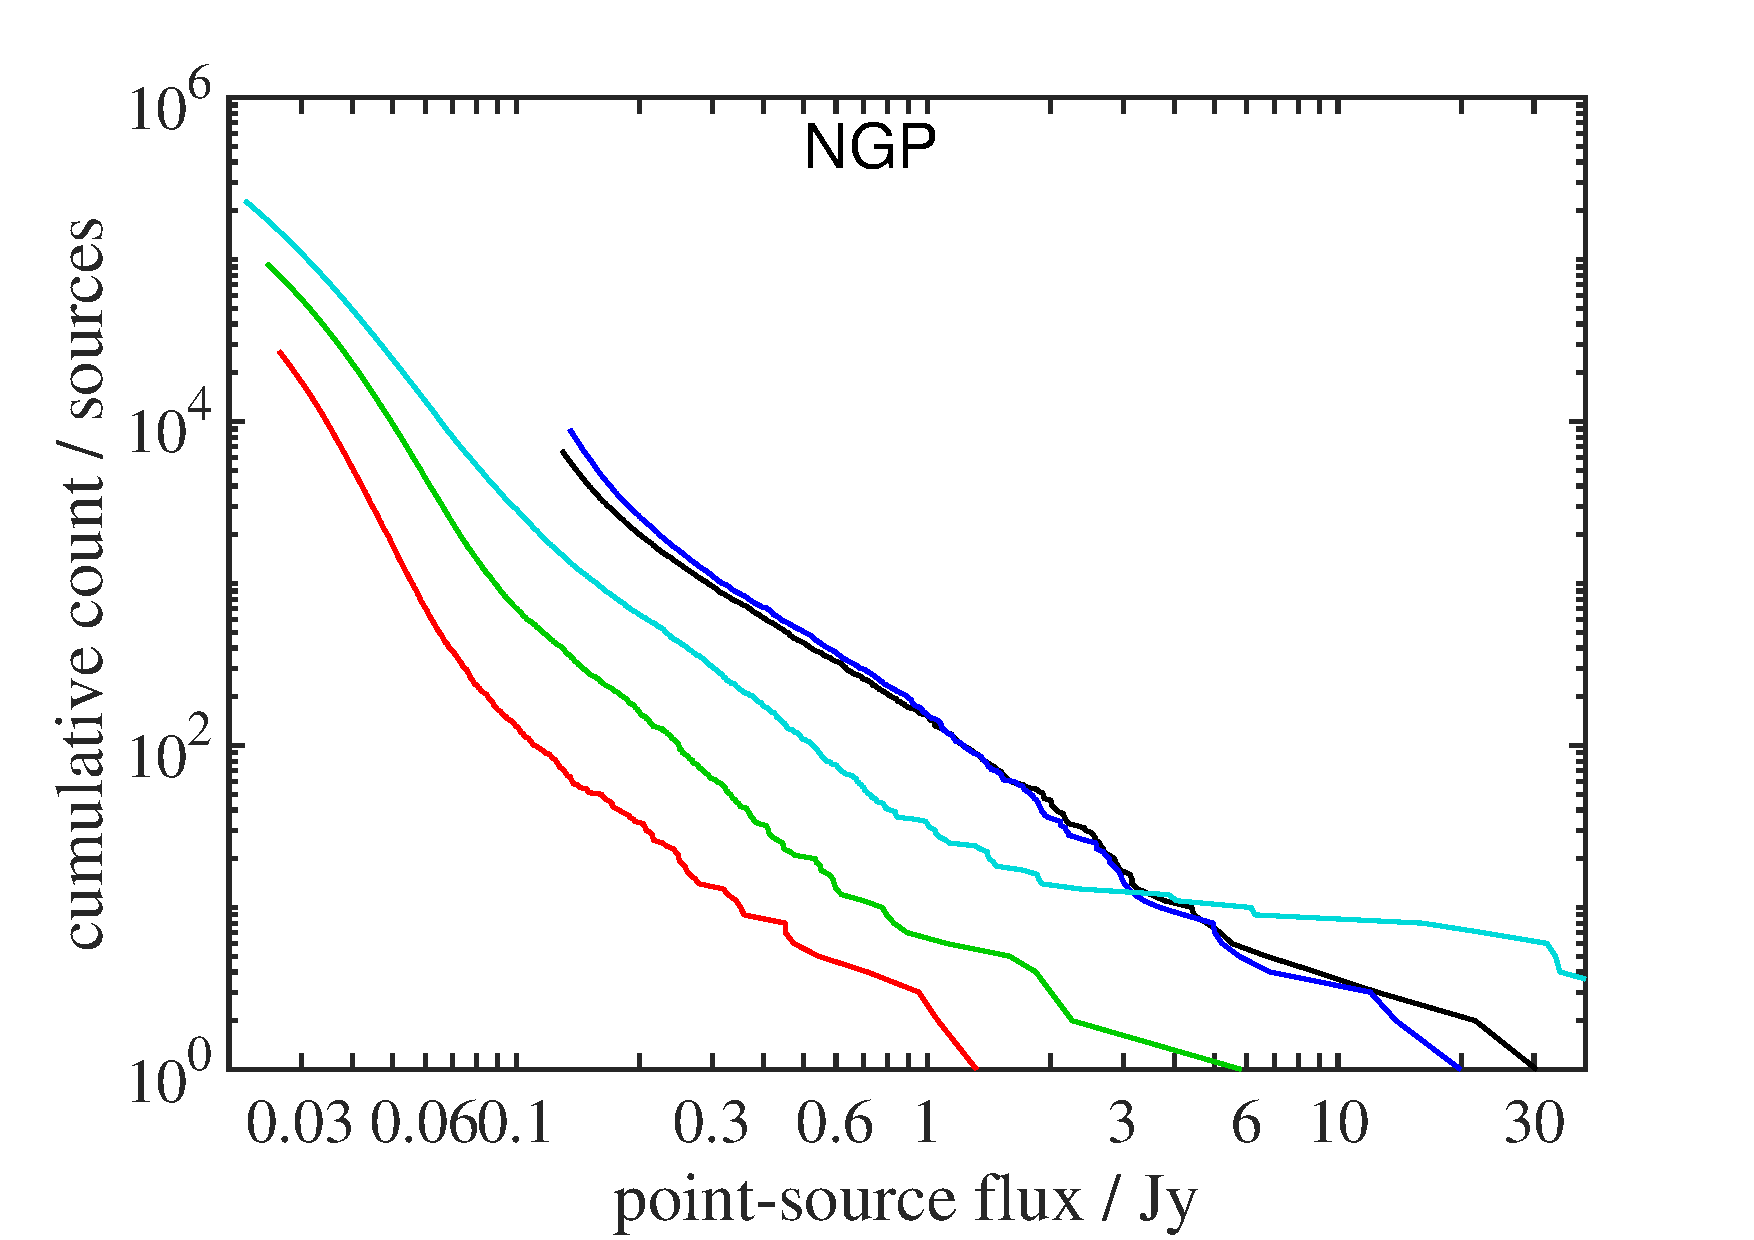
\includegraphics[width=0.5\textwidth]{cum_counts_NGP.pdf}\\
  %(b)\hspace{-1mm}
  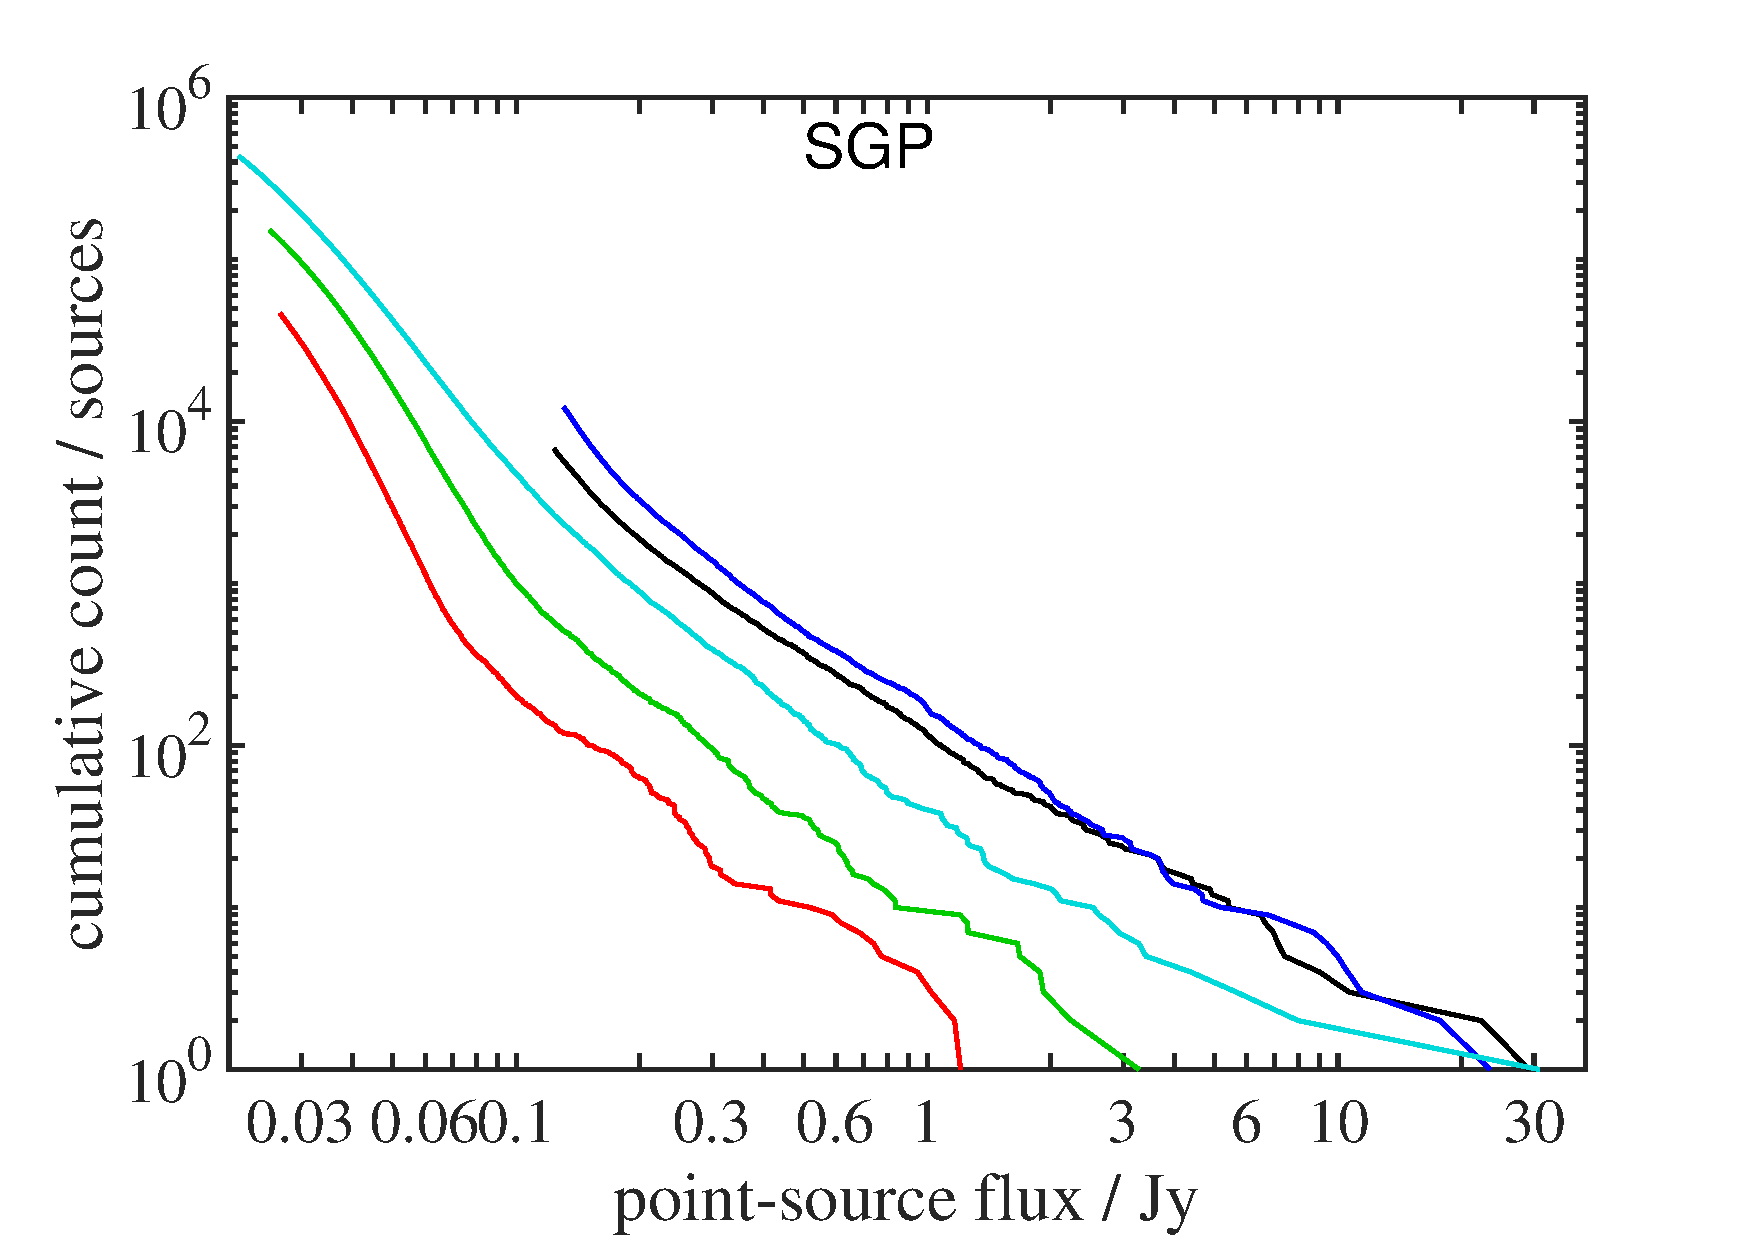
\includegraphics[width=0.5\textwidth]{cum_counts_SGP.pdf}
  \caption{\protect\label{fig_cum_flux} The cumulative number of
    sources as a function of flux at 100\mic (black), 160\mic (blue),
    250\mic (cyan), 350\mic (green) and 500\mic (red). The NGP area is
    shown in the top panel, and the SGP in the bottom panel. The
    counts are plotted only above the limit of 3$\sigma$ in each wave
    band.  }
\end{figure}
% \begin{figure} %3 
% 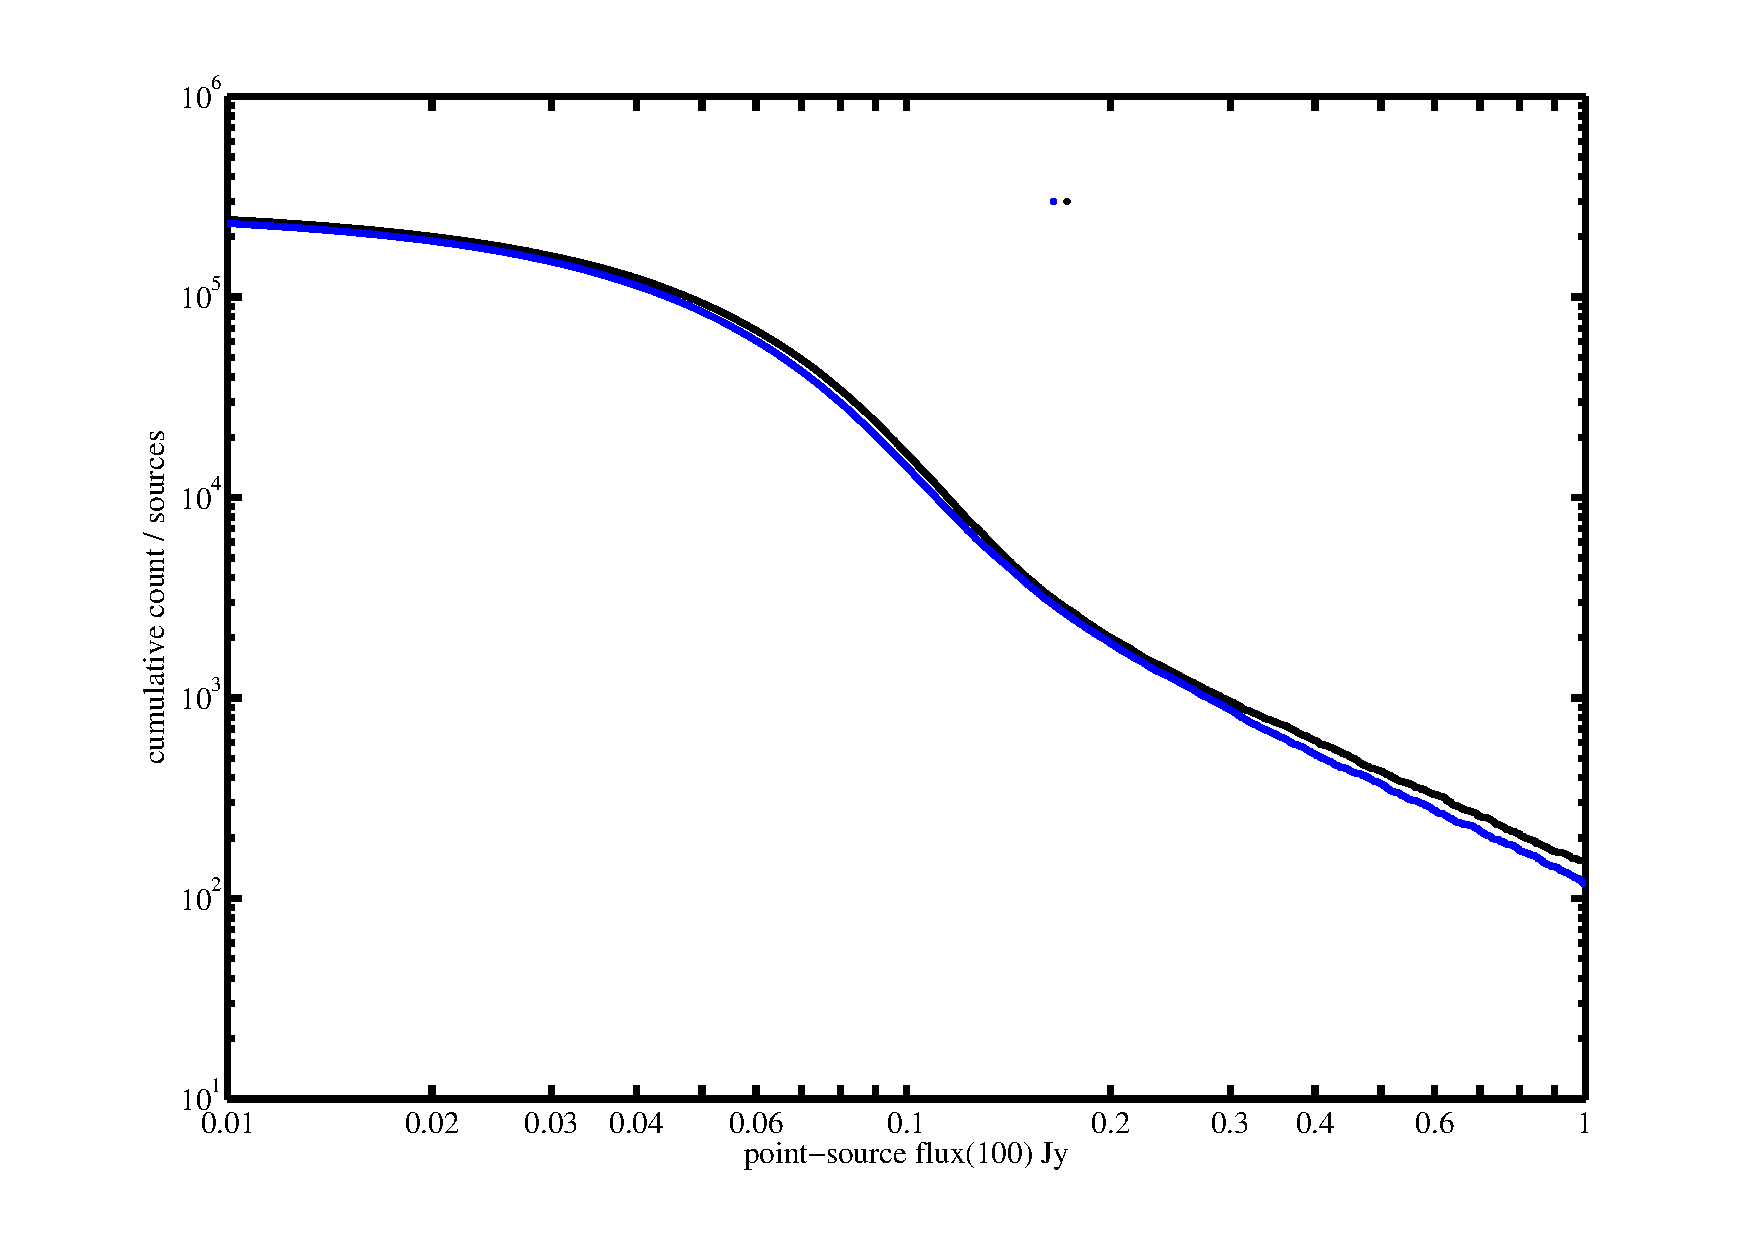
\includegraphics[width=0.42\textwidth,clip,trim={0 9mm 0mm 16mm}]{cum_counts_100.pdf}
% 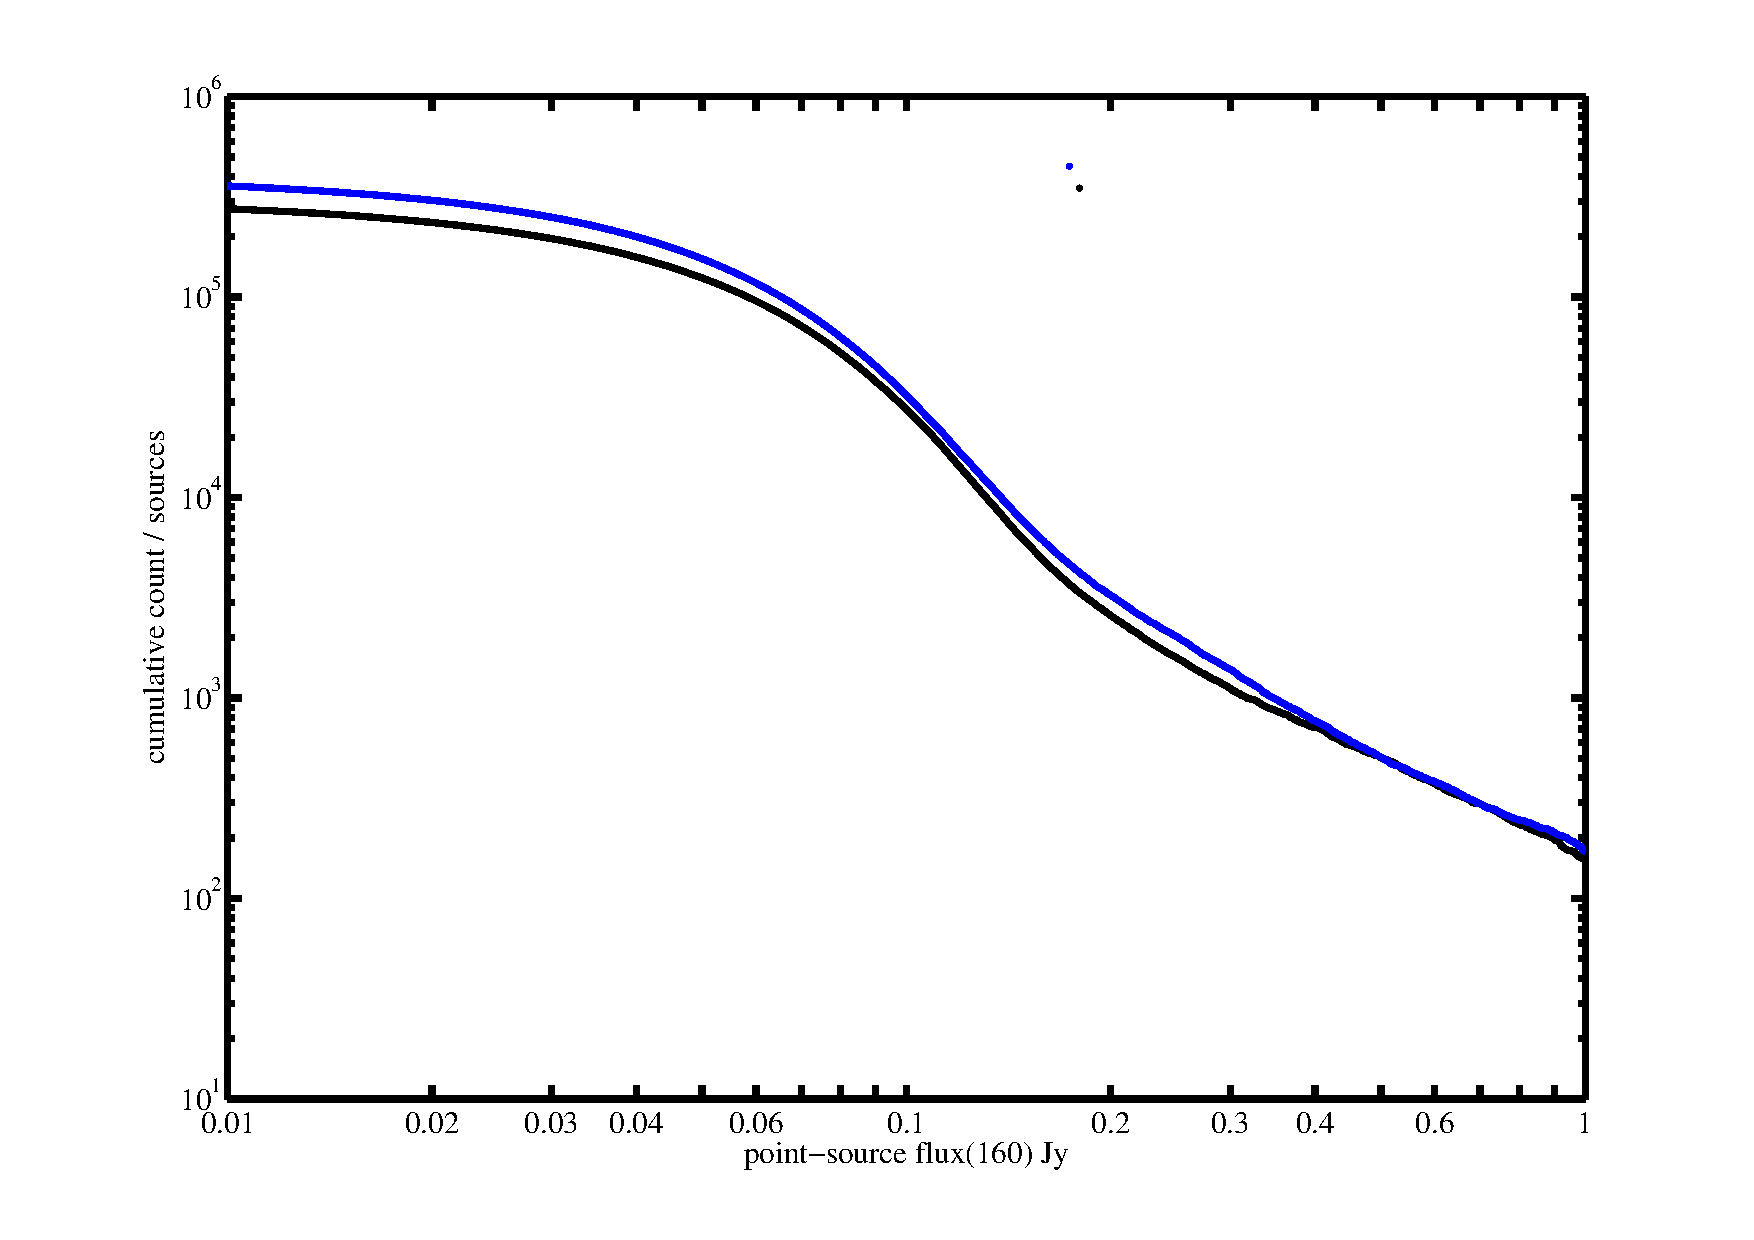
\includegraphics[width=0.42\textwidth,clip,trim={0 9mm 0mm 16mm}]{cum_counts_160.pdf}
% 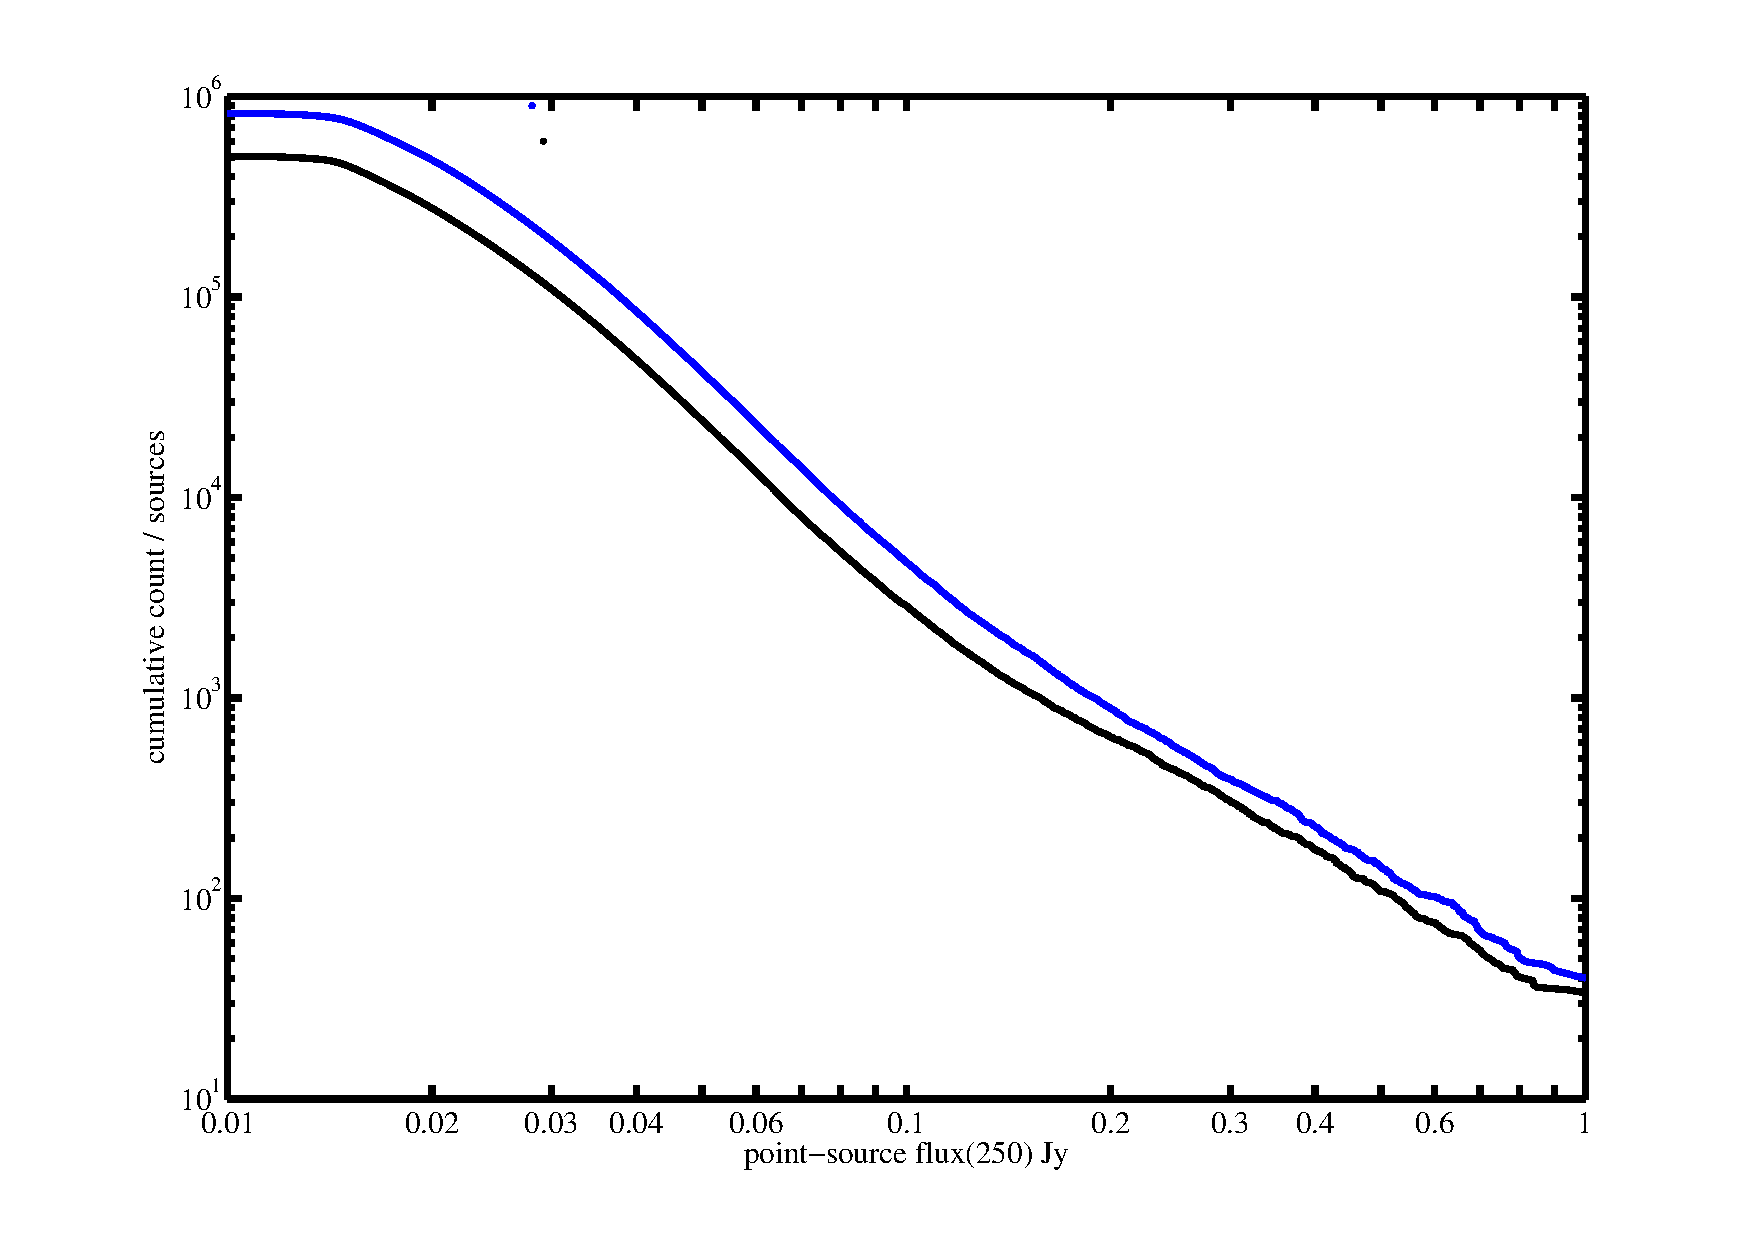
\includegraphics[width=0.42\textwidth,clip,trim={0 9mm 0mm 16mm}]{cum_counts_250.pdf}
% 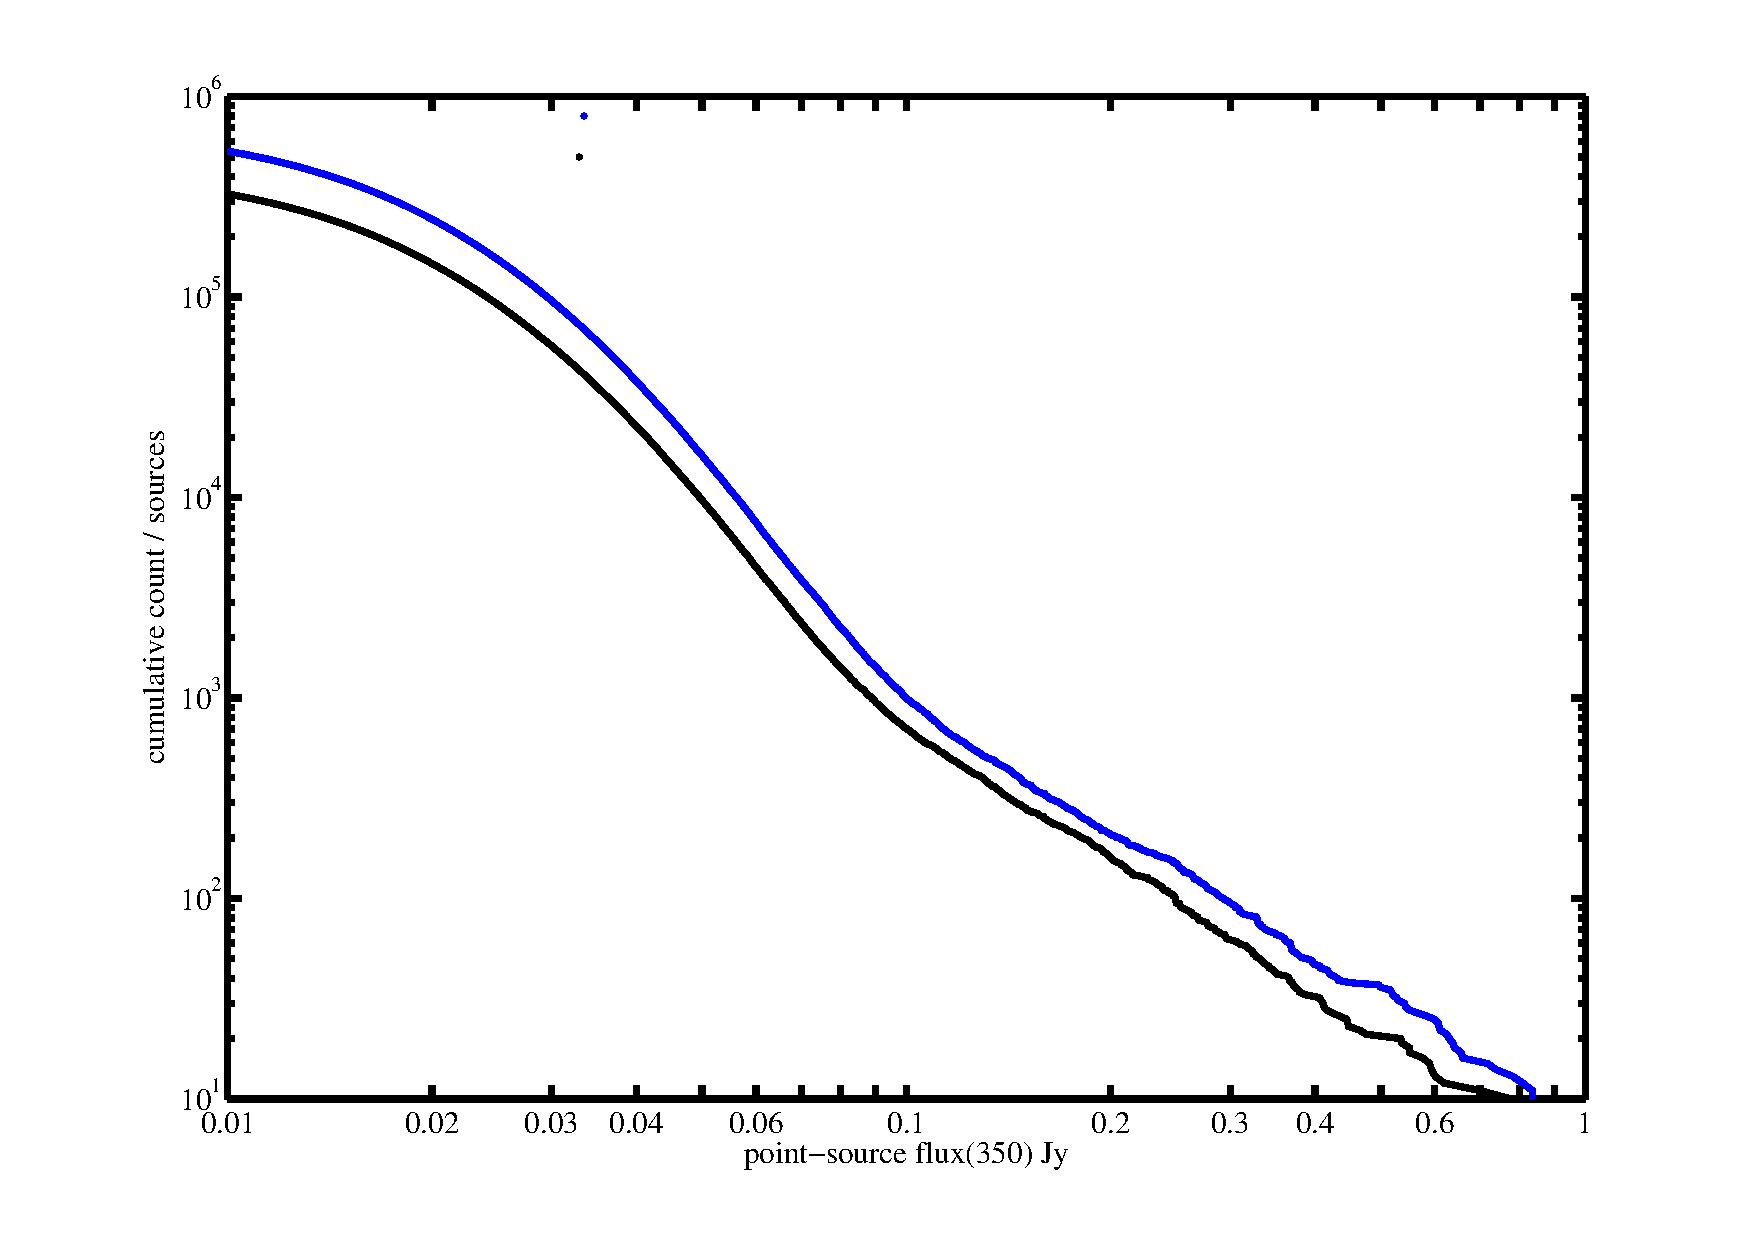
\includegraphics[width=0.42\textwidth,clip,trim={0 9mm 0mm 16mm}]{cum_counts_350.pdf}
% 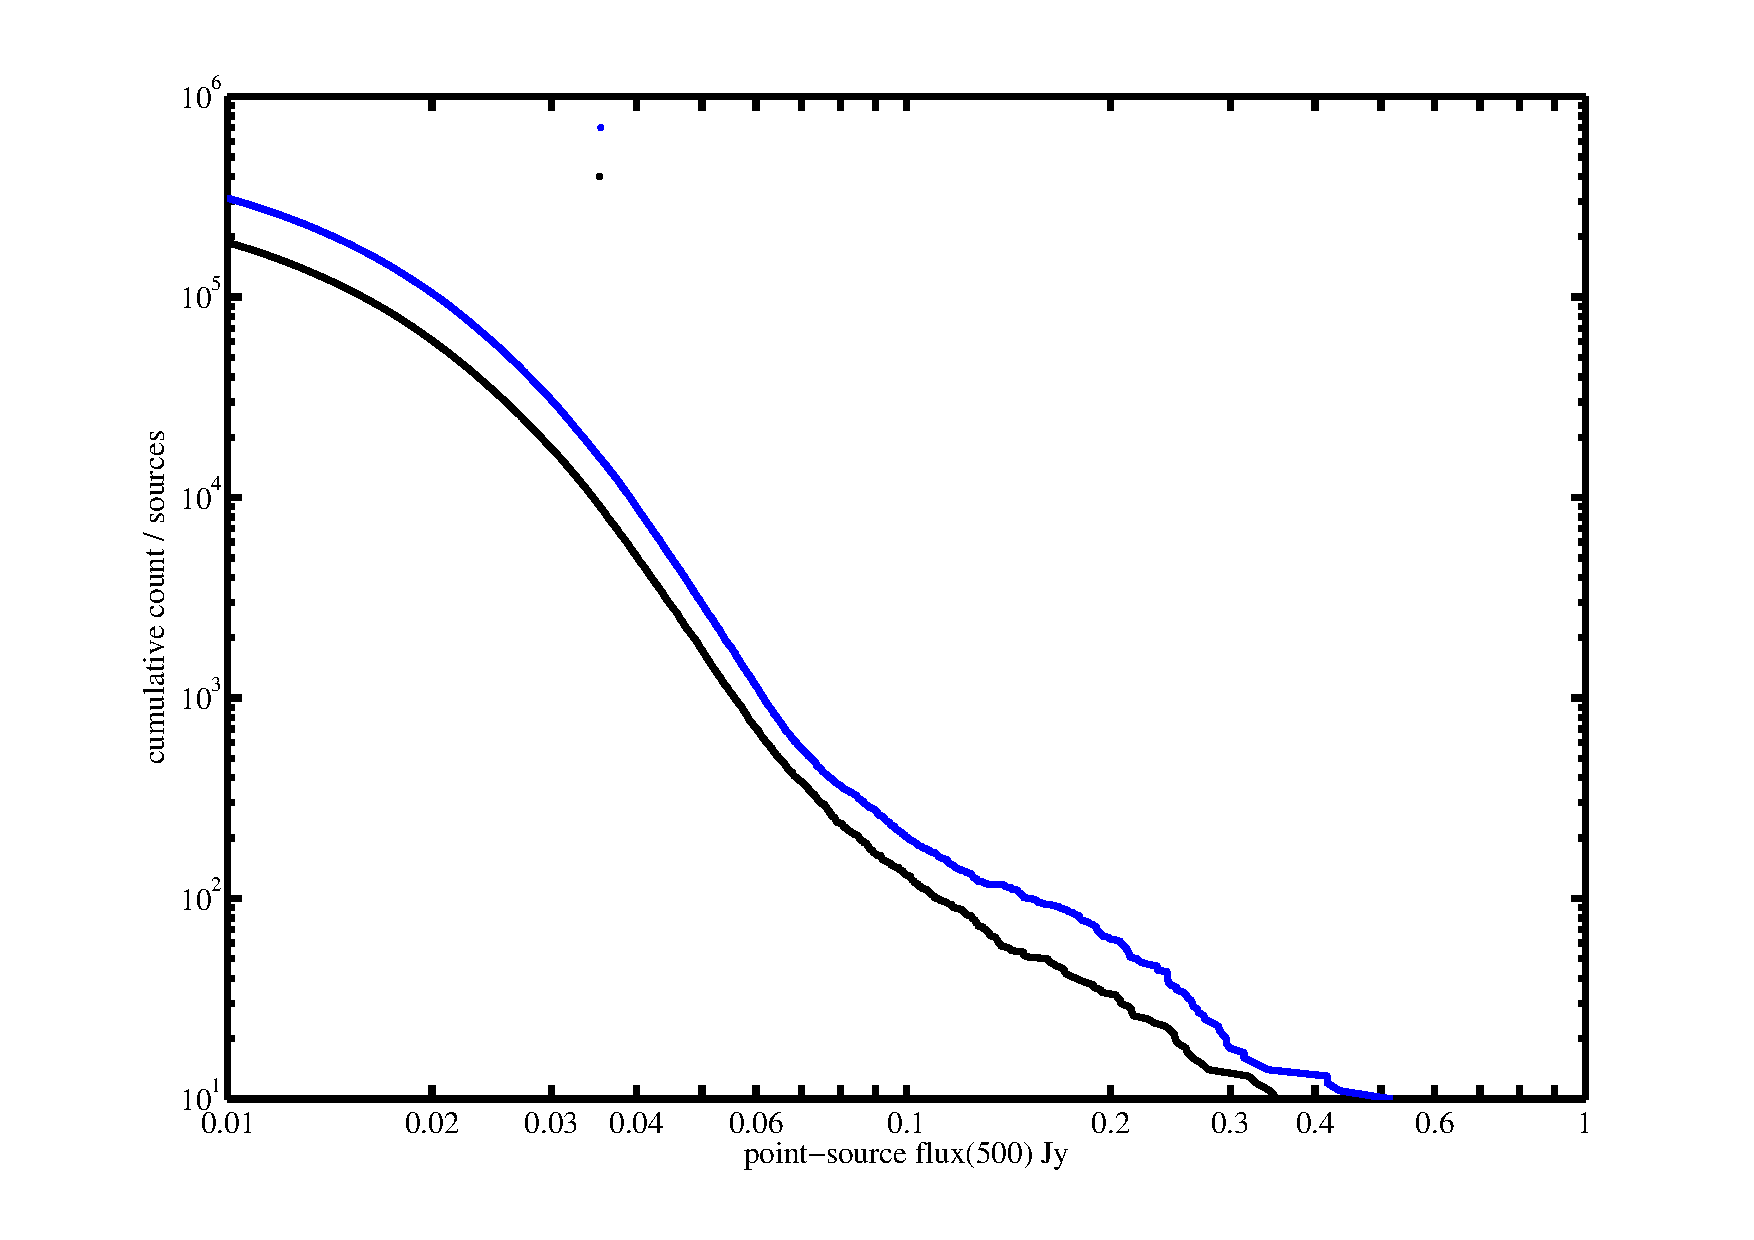
\includegraphics[width=0.42\textwidth,clip,trim={0 9mm 0mm 16mm}]{cum_counts_500.pdf}
% \caption{\protect\label{fig_cum_flux} The cumulative number of sources as a
%   function of flux at 100\mic, 160\mic, 250\mic, 350\mic and 500\mic. The NGP field is
% shown in black; the SGP in blue. %; GAMA9 in magenta; GAMA12 in green; GAMA15 in red.
% }
% \end{figure}

Sources were detected using the MADX algorithm (Maddox et al in prep)
applied to the SPIRE maps.  MADX creates maps of the signal-to-noise
ratio and identifies sources by finding peaks in the signal to noise. The
detection and measurement of fluxes is optimised by using a matched
filter that is applied to both the signal map and the noise map. 

The SPIRE instrumental noise maps are created from the number of
detector passes and the estimated instrumental noise per pass,
$\sigma_{\mathrm inst} /\sqrt{N_ {\mathrm sample}}$, as described in S17 and V16.

%% the 2.5sig cut is instrumental only the 4 sigma includes both inst
%% and confusion
%% flux in other bands measured at optimal position, as defined from
%% the 250micron maps; there is a clean process for each band
%% individually
 
Since the noise consists of both instumental noise and
confusion noise from the background of undetected sources, we follow
the approach of Chapin et al (2011) to calculate the optimal matched
filter in each of the three SPIRE bands. Details of estimation and
form of the matched filter are discussed in V16.  The resulting
matched filters are slightly more compact than the corresponding PSFs,
and have slightly negative regions outside the FWHM.  

In the first step of the source detection, peak pixels which have
values $>2.5\sigma$ in the filtered 250\mic map are considered as
potential sources. At this stage only the instrumental noise is
included in the noise estimate. The source position is determined by
fitting to the pixels around the peak in the 250-\mic map. Then the
flux in each band is estimated using a bicubic interpolation to the
exact position in each filtered map. This means that there is a
scatter compared to the original single pixel value, with some sources
being assigned fluxes below the original $2.5\sigma$ cut. Also, for
the 350\mic and 500\mic bands, the scatter can be fairly large, and
the estimated fluxes for some low signal-to-noise sources are actually
negative.  When each source has been measured, a point source profile,
scaled to the estimated flux is subtracted from the data, so flux from
that source cannot be double-counted in other sources that may be
nearby. For each band, sources are sorted in order of decreasing
brightness, so that the brighter sources are subtracted from the map
before the measurement of fainter sources.  Only sources detected
above 4 $\sigma$ in any of the SPIRE bands are retained for the final
catalogue. For this cut, the confusion noise as calculated in Section
3 is added in quadrature to the instrumental noise to give an estimate
of the total noise.

For the two PACS bands we prefer to use aperture based photometry for
all sources, because the PACS psf for our fast-parallel scan mode data
is not well determined near the peak. Also the positional uncertainty
from the 250\mic detection combined with the higher angular resolution
of the PACS maps means that the estimated 250\mic position is likely
to miss the peak in PACS map, and hence we would underestimate the
flux if we used a matched filter approach as for the longer wavelength
SPIRE bands. We set the PACS apertures to have a radius equal to the
FWHM of the psf, 11.4 arc seconds for 100\mic and 13.7 arc seconds for
160\mic.  These are corrected to total fluxes using the EEF
corrections presented in V16, and available at {\tt
  http://www.h-atlas.org/}.  We make a further correction to allow for
the bias caused by the expected random positional errors between the
SPIRE 250\mic and PACS maps.
For sources in the NGP where we have identified a reliable optical
counterpart using the maximum likelihood approach presented in
F17, we use the optical position to place the
apertures, as the optical positions are more precise that the SPIRE
250\mic estimates. 

\subsection{Extended sources} 

This approach gives optimal flux estimates for point sources, but will
seriously underestimate the flux for extended sources. We use the
sizes of optical counterparts to determine which sources are likely to
be extended, and sum the flux within an aperture to estimate the total
flux of the source. Extended source aperture fluxes are calculated in
this way for both PACS and SPIRE bands. 

In the NGP area, we use optical identifications
with reliability $R>0.8$, from F17.  Sources are
considered likely to be extended if the SDSS measured 90\% Petrosian
radius in the $r$ band, $\mathtt{petroR90\_r}$, is greater than 8.6
arc seconds. In our previous data release (V16) we based our apertures
on the SDSS DR7 $\mathtt{isoA\_r}$, but this parameter is not
available in later SDSS releases. We compared the various radius
measures available, and found that a simple scaling of
$\mathtt{petroR90\_r}$ provides a robust size measurement that is
closely related to $\mathtt{isoA\_r}$, so $\mathtt{isoA\_r} \approx
1.156 \ \mathtt{petroR90\_r}$.  We have simply used the same methods
as Valiante et al (2016), but with $\mathtt{isoA\_r}$ replaced by
$1.156 \ \mathtt{petroR90\_r}$. So, the radius of the apertures are
defined as
\begin{equation} 
r_\mathrm{ap} = \sqrt{ \mathtt{FWHM}^2 + {(1.156
    \ \mathtt{petroR90\_r})}^2}\ , 
\end{equation}
where $\mathtt{FWHM}$ is the full-width half-max of the point-spread
function for the passband being measured.  

For the SGP area no SDSS data exists, and we chose to use sizes
from the 2MASS survey. We have not performed a full likelihood
identification analysis, but have simply looked at the largest
galaxies to provide better fluxes for the largest galaxies. 
%Once the VISTA KIDS and VST VIKING surveys are available we plan to run a maximum
%likelihood cross-identification analysis as for the GAMA and NGP
%data. 
In order to derive aperture radii that are similar to the other HATLAS
fields, we compared the 2MASS super-coadd 3-sigma isophotal semi-major
axis radius to the SDSS $\mathtt {isoA\_r}$ measurements. We found that a
simple scaling $\mathtt{isoA\_r} \approx 1.96 \ \mathtt{sup\_r\_3sig}$
was a reasonable approximation, and so used aperture radii, $r_{ap}$
given by, 
\begin{equation} 
r_\mathrm{ap} = \sqrt{ \mathtt{FWHM}^2 + {(1.96
    \ \mathtt{sup\_r\_3sig})}^2}\ .
\end{equation}

For both the NGP and SGP areas, the aperture flux is used for a source
if it is significantly larger than the point-source estimate, ie
\begin{equation} 
F_\mathrm{ap}- F_\mathrm{ps}>\sqrt{\sigma_\mathrm{ap}^2-\sigma_\mathrm{ps}^2}
\ .
\end{equation}

Since the maps have been background subtracted, we do not make any
further background subtraction when performing the aperture
photometry. We do make a correction to the aperture fluxes to allow
for flux outside the aperture using the SPIRE and PACS EEF.

Overall we measure aperture fluxes for 1850 sources in the NGP. For
some sources which are barely resolved, the point source flux may be
the better flux estimate, and be chose the 'best' flux estimate to be
the aperture flux only if it is sginificantly higher than the point
source estimate. 

We have visually checked the apertures for the largest and brightest
sources, and in some cases (how many?) we have adjusted the apertures
to better match the Herschel imaging. 

\subsection{Flux distributions} 

The observed number of sources as  function of flux in the PACS and
SPIRES bands is shown in figure~\ref{fig_cum_flux}. The fluxes are
subject to boosting as described in V16, and need a statistical
de-boosting correction before  comparing to model predictions. 


\subsection{Colour Corrections} 
 
The SPIRE maps are calibrated assuming the source spectral energy 
distribution (SED)  varies with frequency as $\nu^{-1}$. For different SED
shapes colour corrections $K_{\mathrm ColP}$ are required, as
presented in Tables 5.6 and 5.7 in the SPIRE Handbook. 

Since the beam areas depend on the source SED, and extended source
photometry depends on maps in Jy/pixel rather than Jy/beam, the
extended source fluxes require colour corrections $K_{\mathrm ColP}$,
as presented in Tables 5.6 and 5.7 in the SPIRE Handbook.

As with SPIRE, the PACS flux density calibrations are based on the
assumption that flux density is proportional to $\nu^{-1}$, and
a correction is required for sources which follow a different SED. The
required corrections are described in the PACS Colour-Correction
document\footnote{\tt{http://herschel.esac.esa.int/twiki/pub/Public/
  PacsCalibrationWeb/cc\_report\_v1.pdf}}).

We have made statistically reliable identifications to optical
galaxies from the SDSS and UKIDSS-LAS catalogues, but we have not
attempted to produce matched aperture photometry. For the optical
photometry from SDSS we use their {\tt ModelMag} measurements; for the
NIR photometry from LAS, we use the petrosian magnitude
measurements. Both should approximated total magnitudes for the
sources, but caution is advised if the photometry is used to constrain
the galaxy SEDs without further corrections.

\section{Flux uncertainties} 

\begin{figure*} %4 
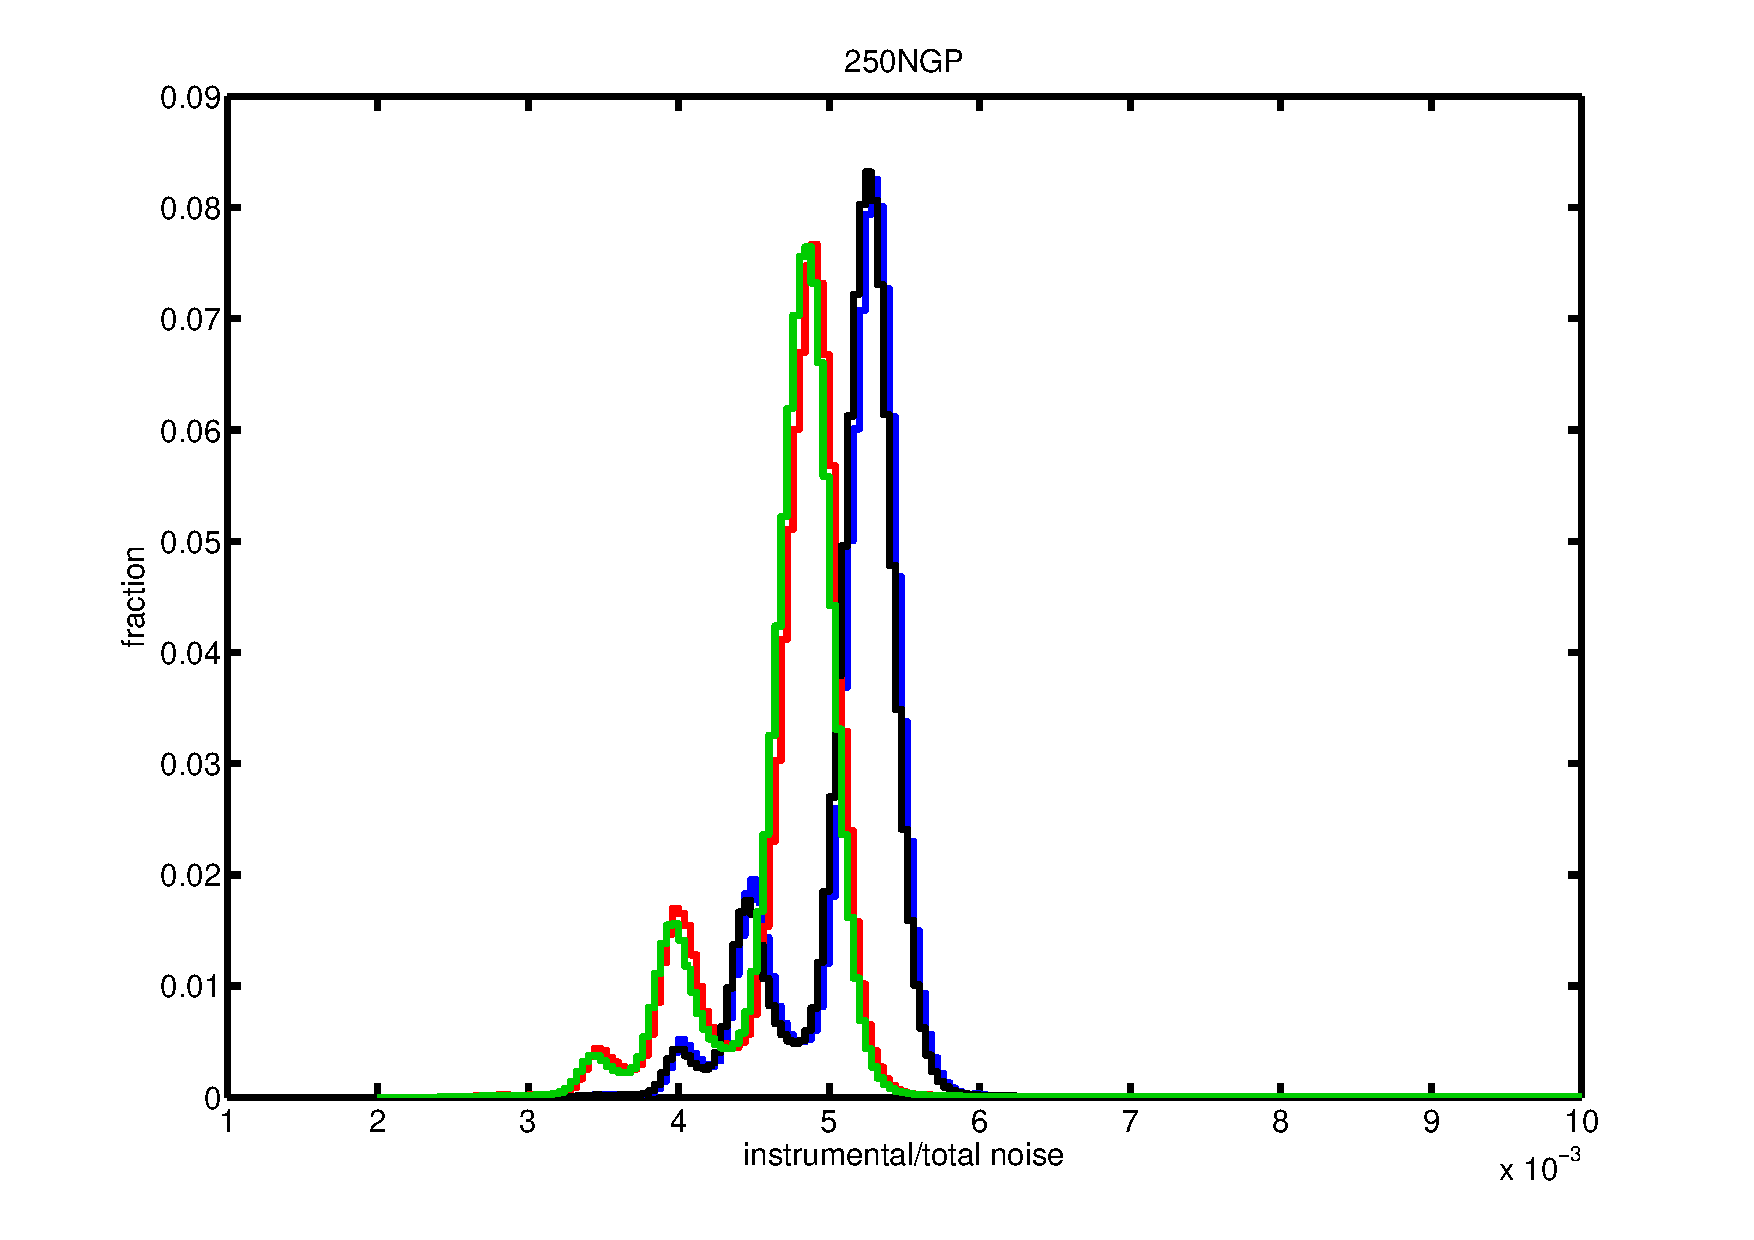
\includegraphics[width=0.3\textwidth]{flux_noise_250NGP.pdf}
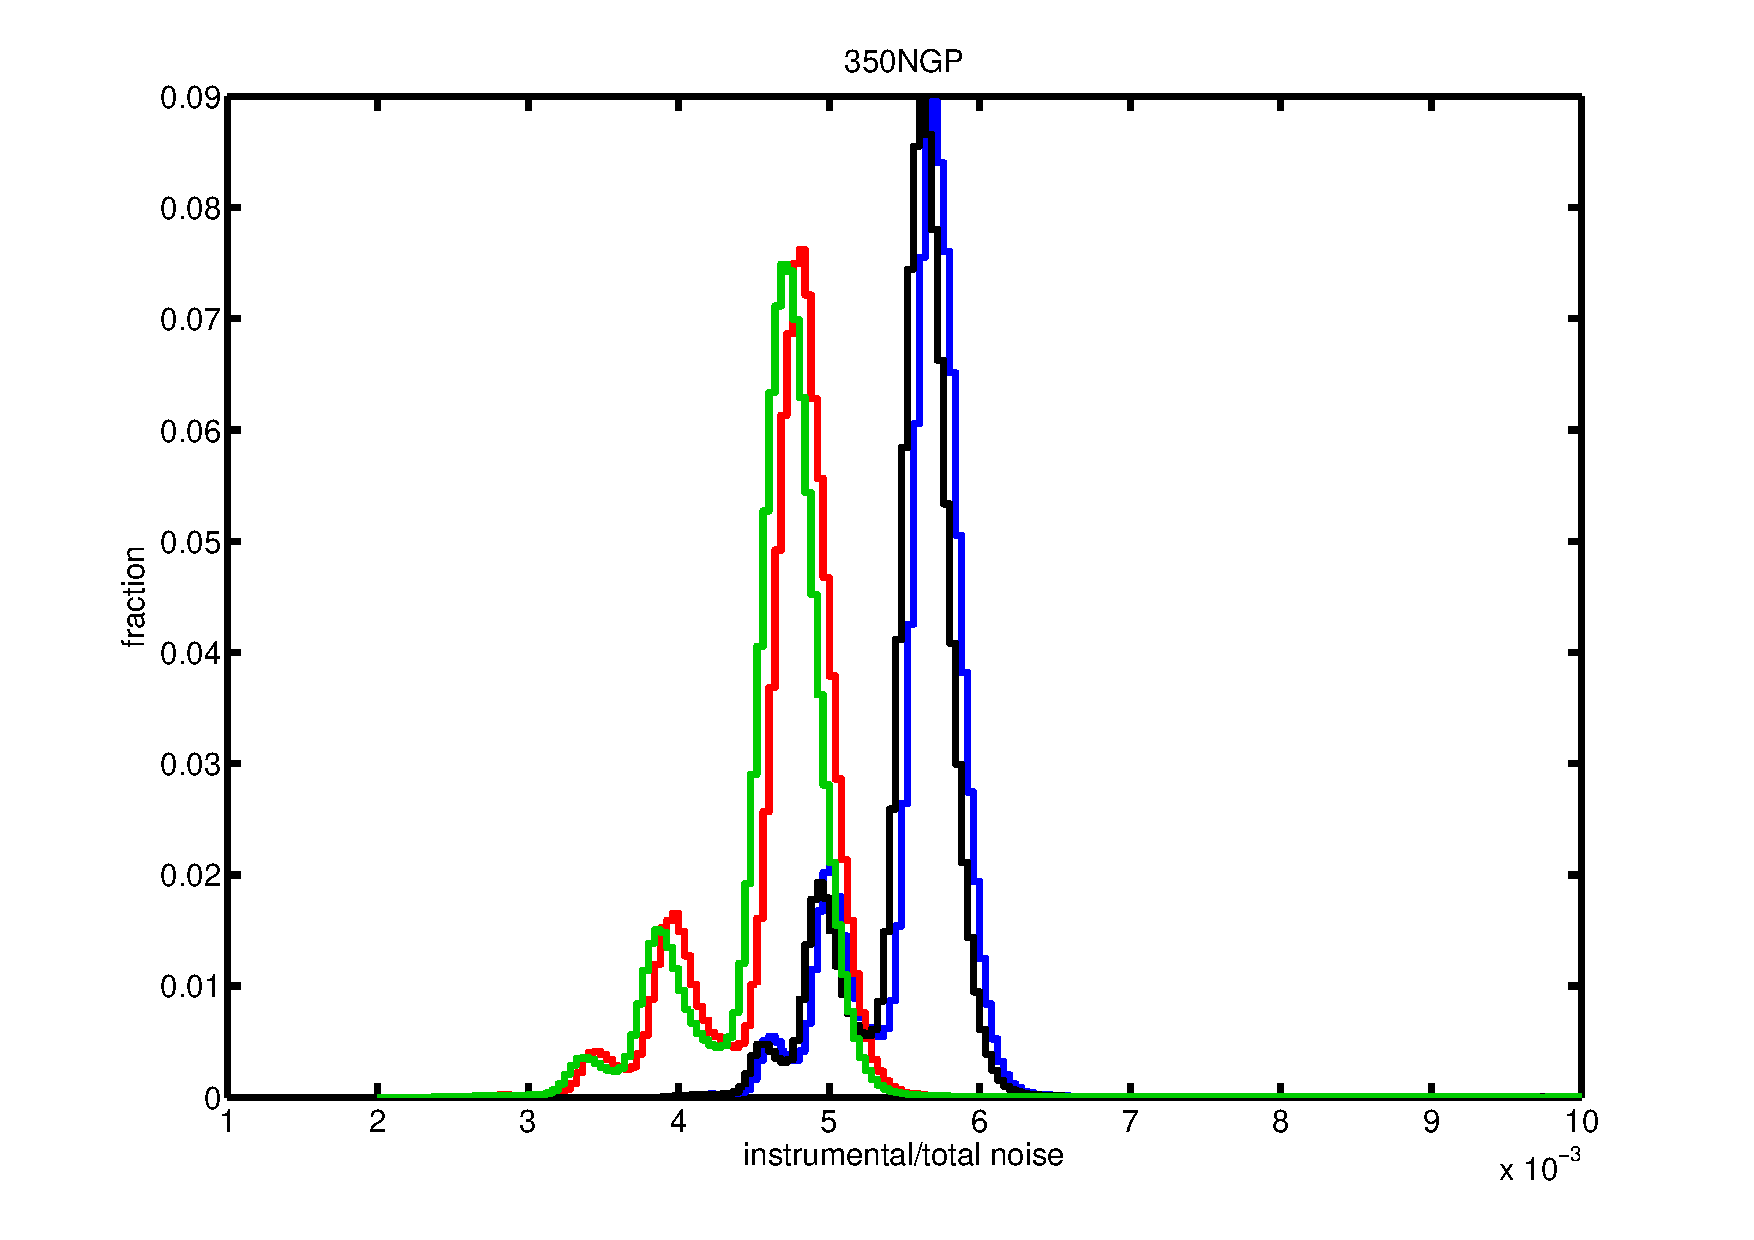
\includegraphics[width=0.3\textwidth]{flux_noise_350NGP.pdf}
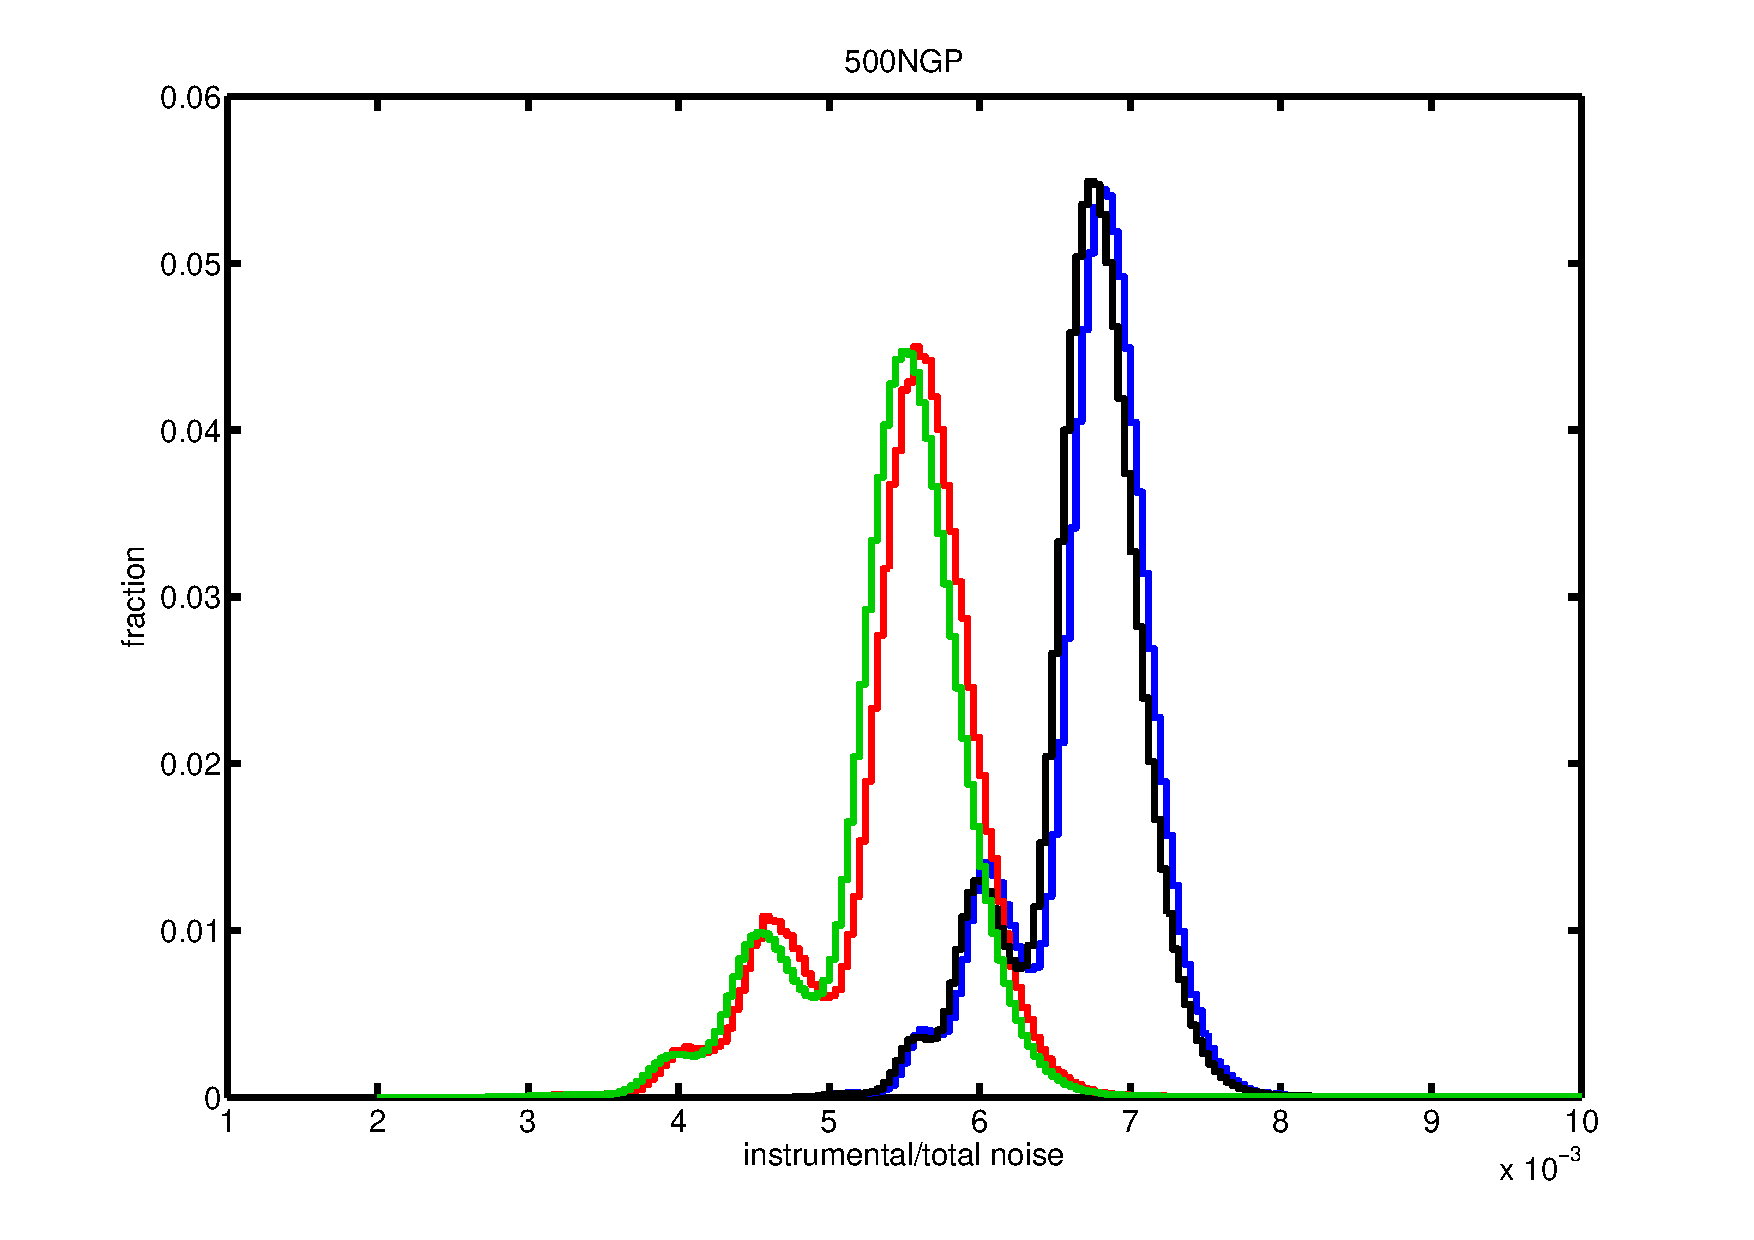
\includegraphics[width=0.3\textwidth]{flux_noise_500NGP.pdf}
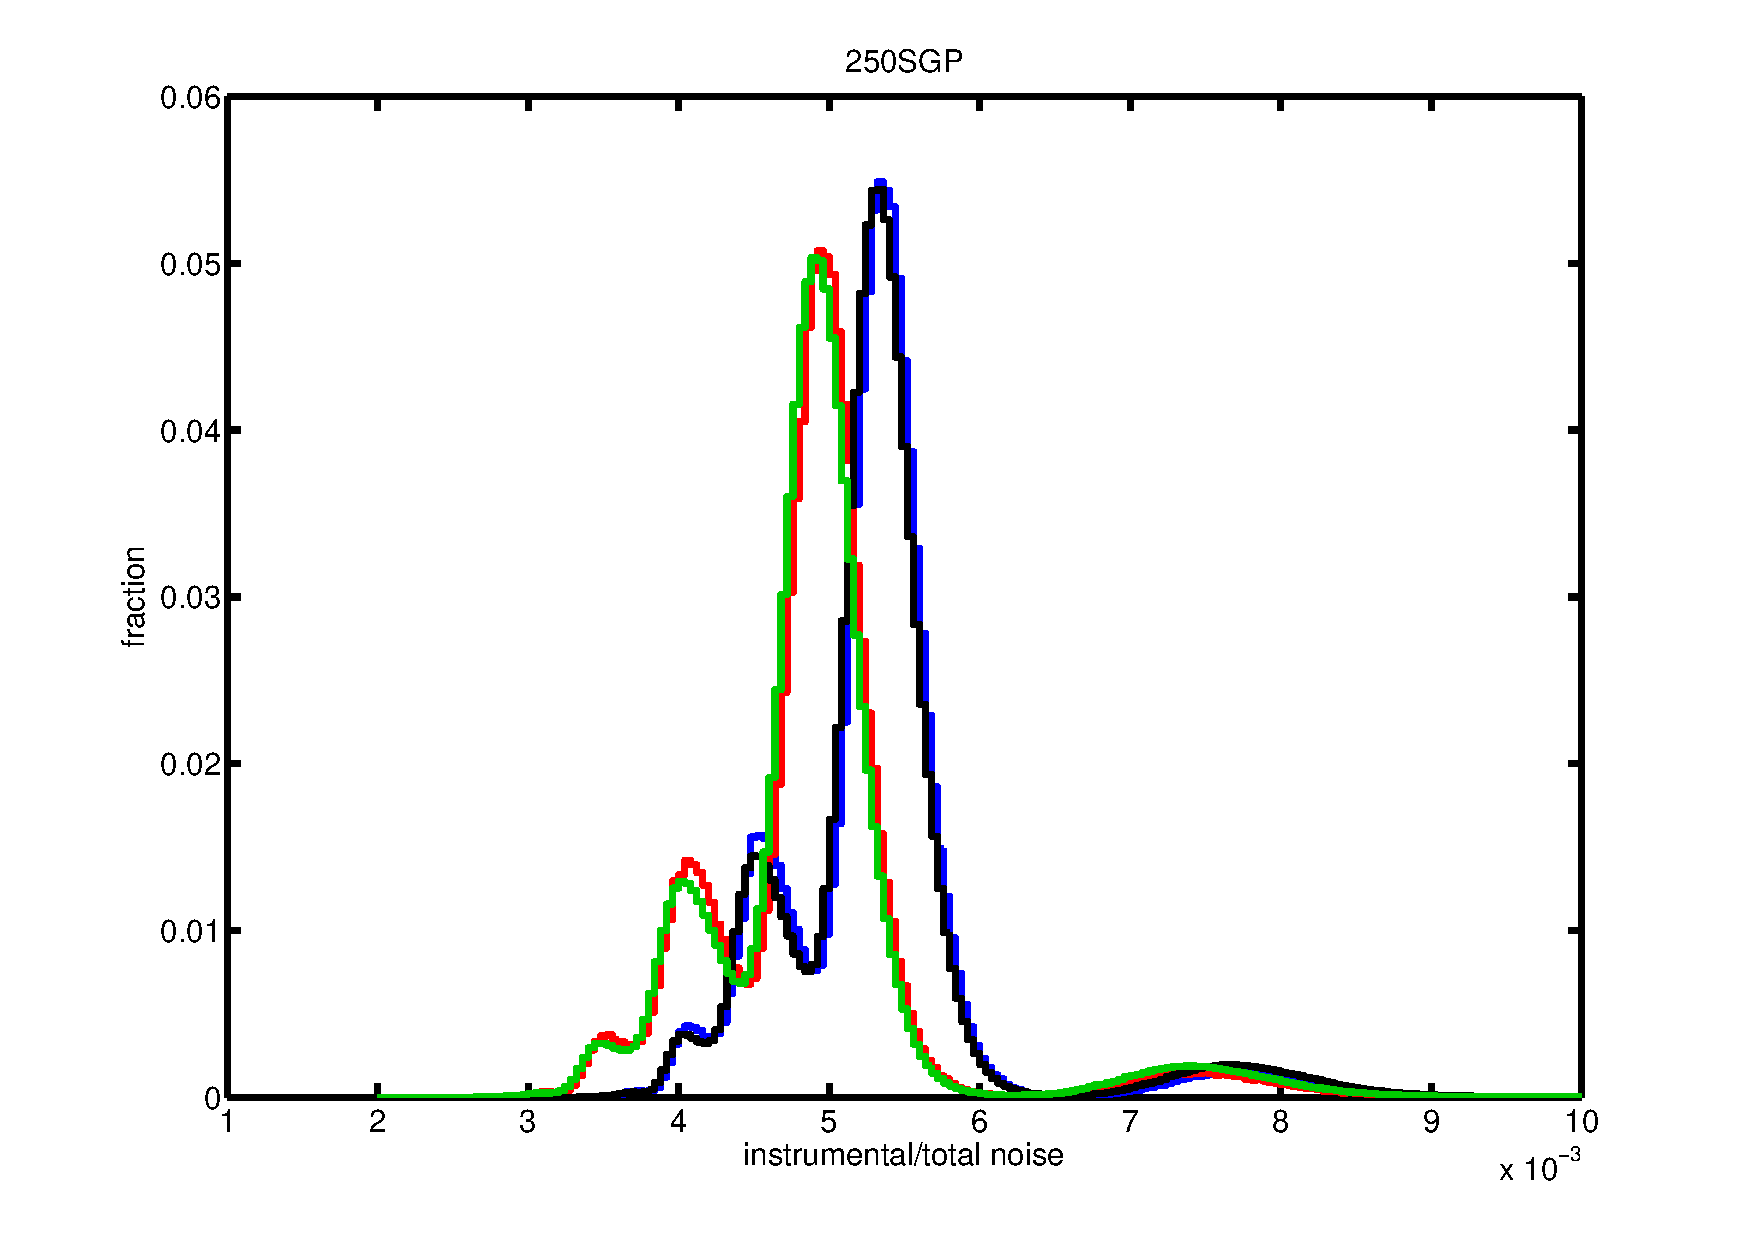
\includegraphics[width=0.3\textwidth]{flux_noise_250SGP.pdf}
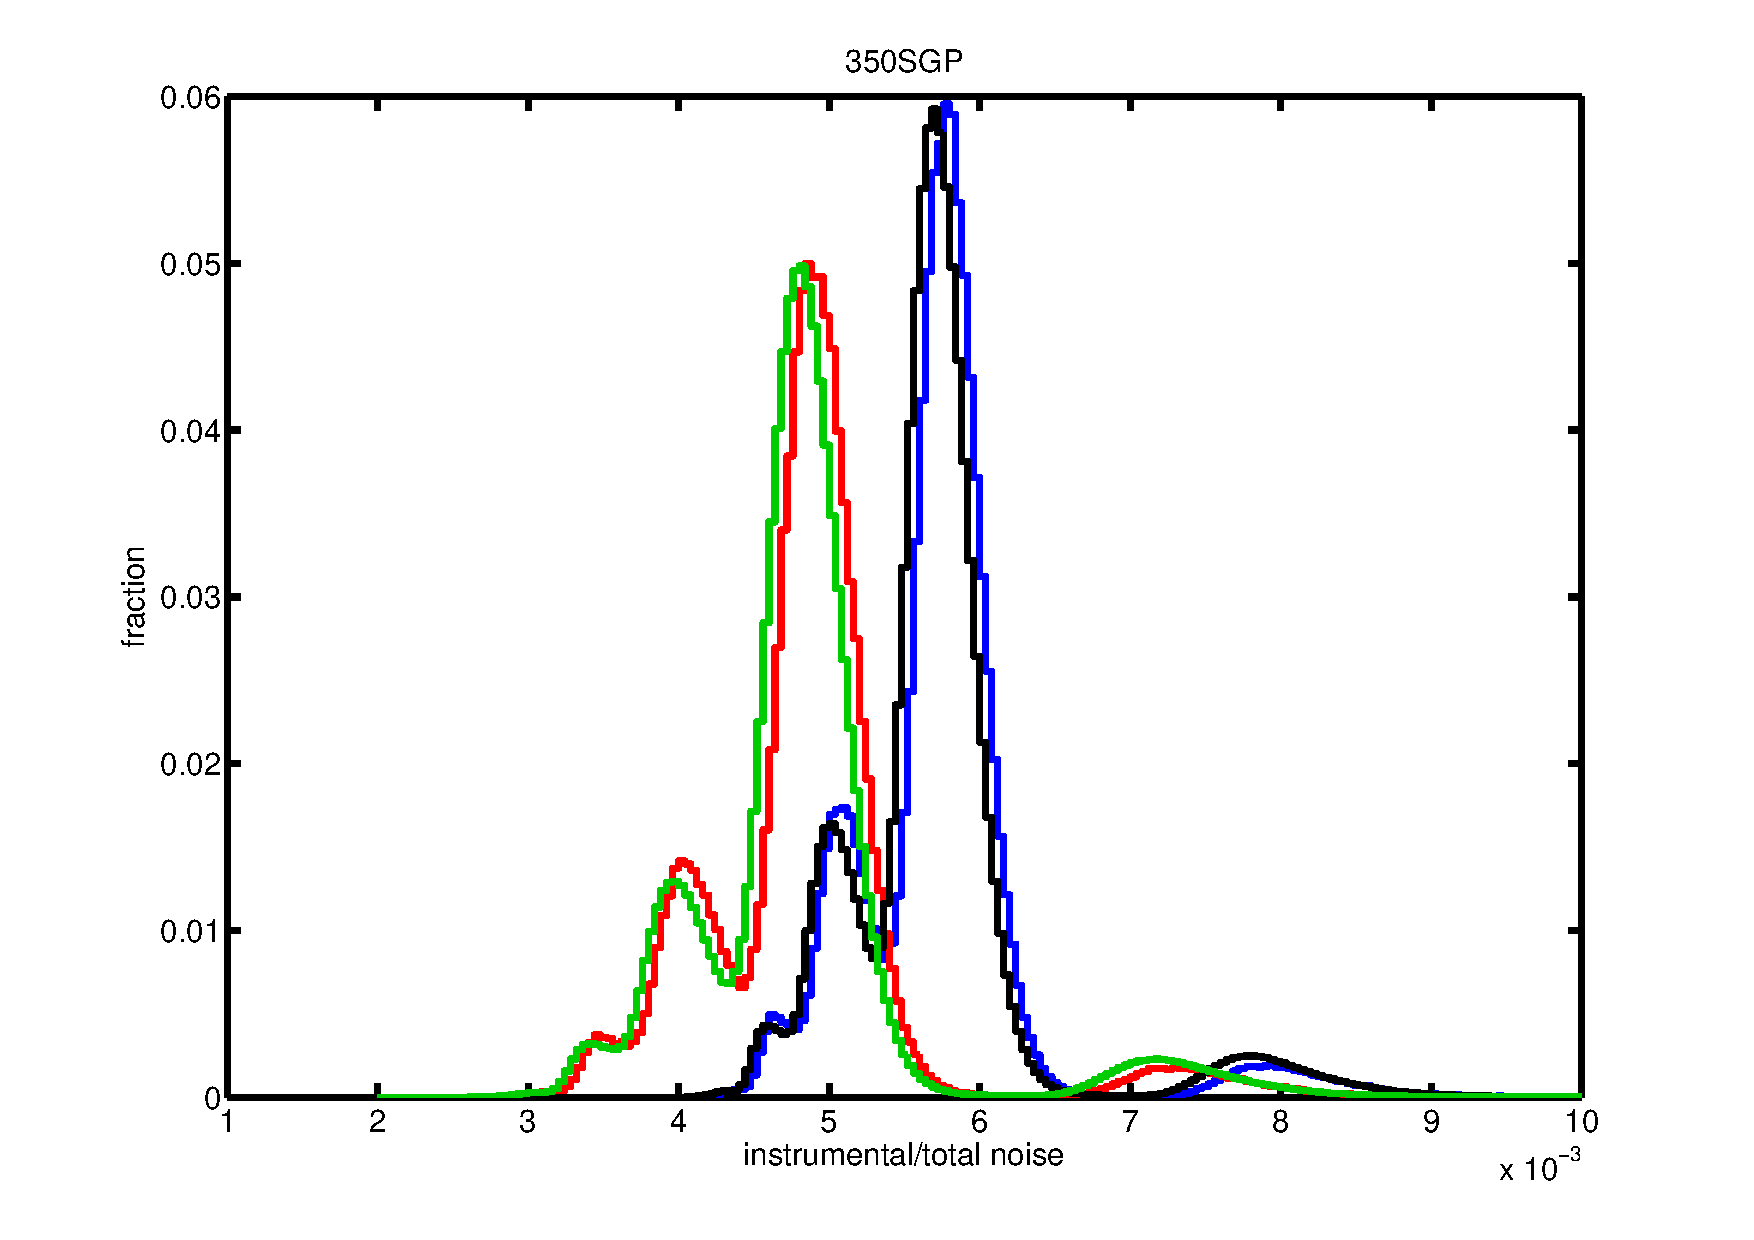
\includegraphics[width=0.3\textwidth]{flux_noise_350SGP.pdf}
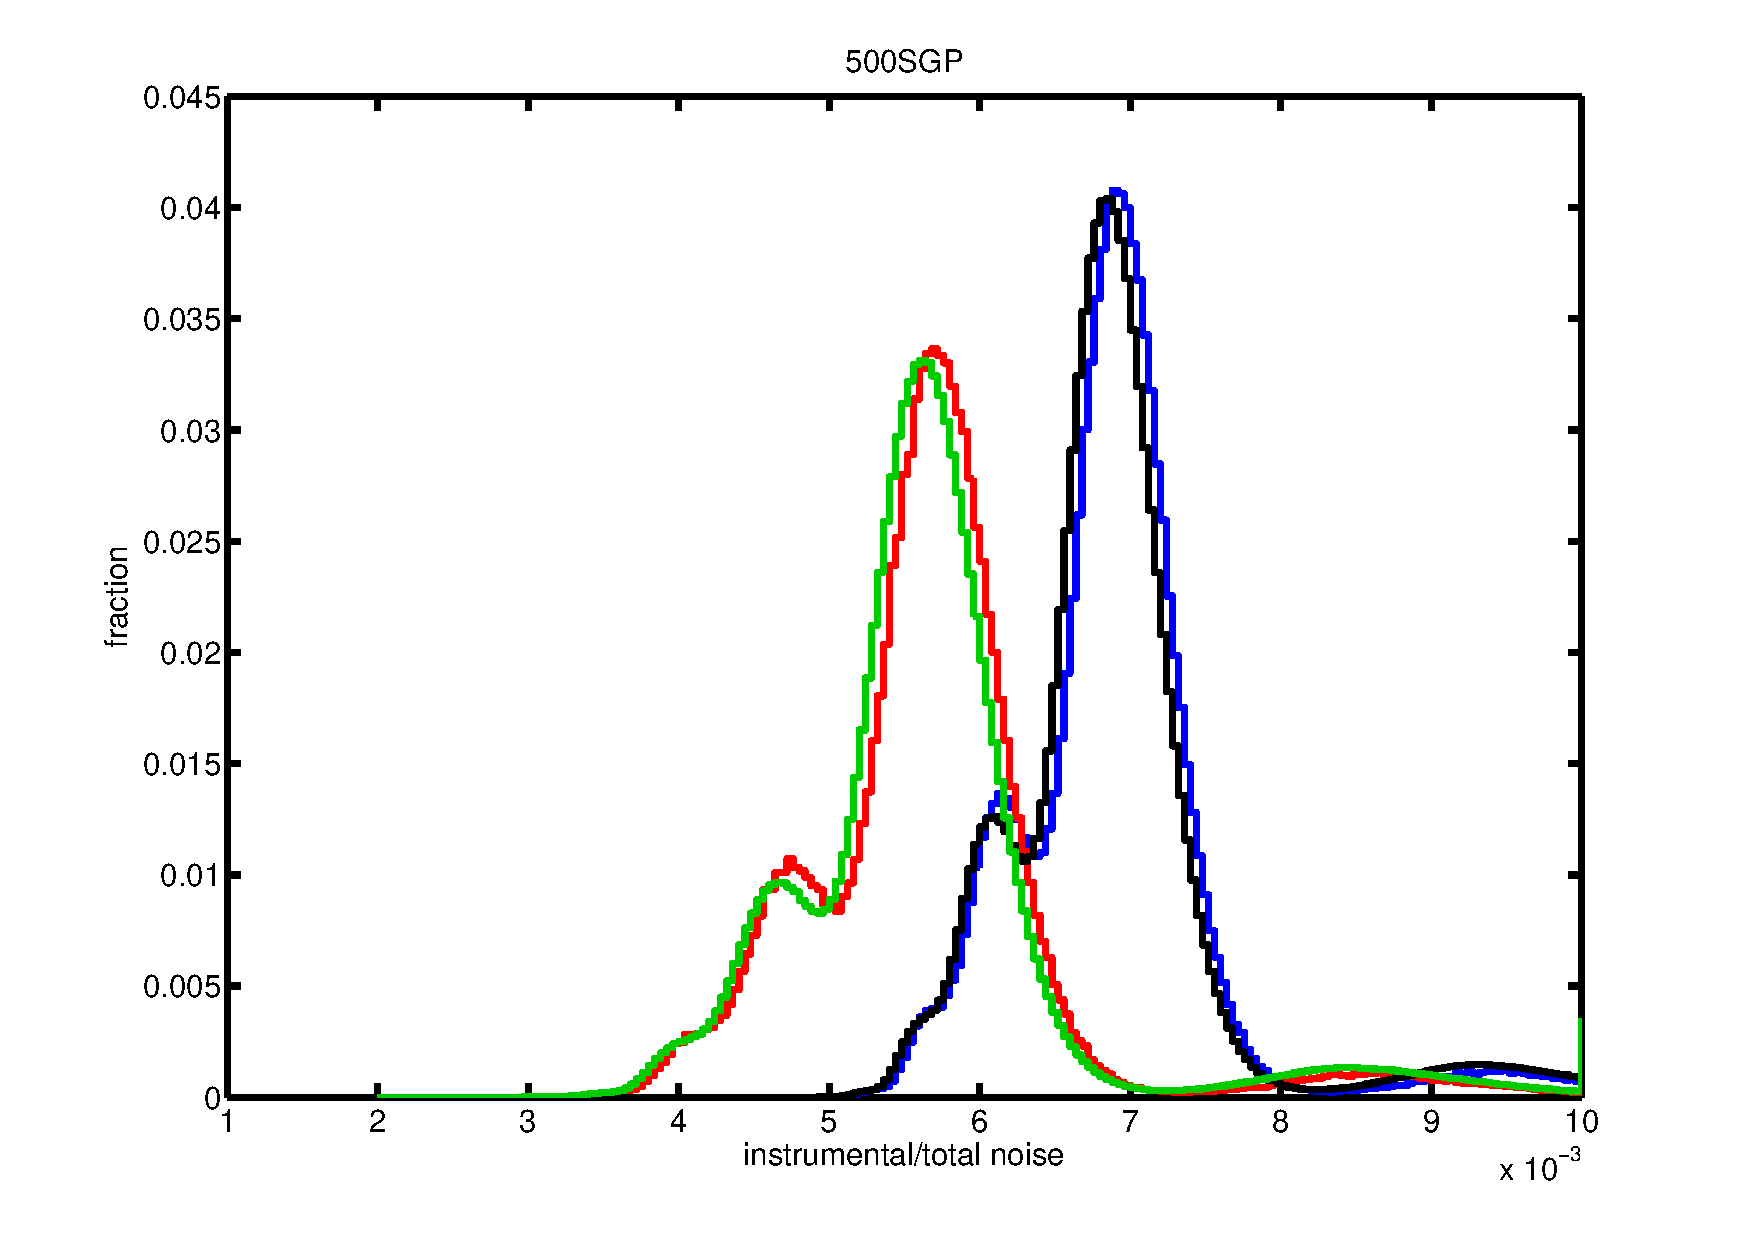
\includegraphics[width=0.3\textwidth]{flux_noise_500SGP.pdf}
\caption{The distribution of instrumental and total noise on the
  measured 250\mic, 350\mic and 500\mic fluxes for the NGP and SGP fields.
  Green shows the instrumental noise estimated for each map pixel; red is
  the instrumental noise for each source; black is the total noise
  from map pixels, and blue is the total nose for sources. 
The single scan area is visible as the small peak of sources and
pixels with higher noise. }
\label{fig_noises}
\end{figure*}

\begin{figure} %5 
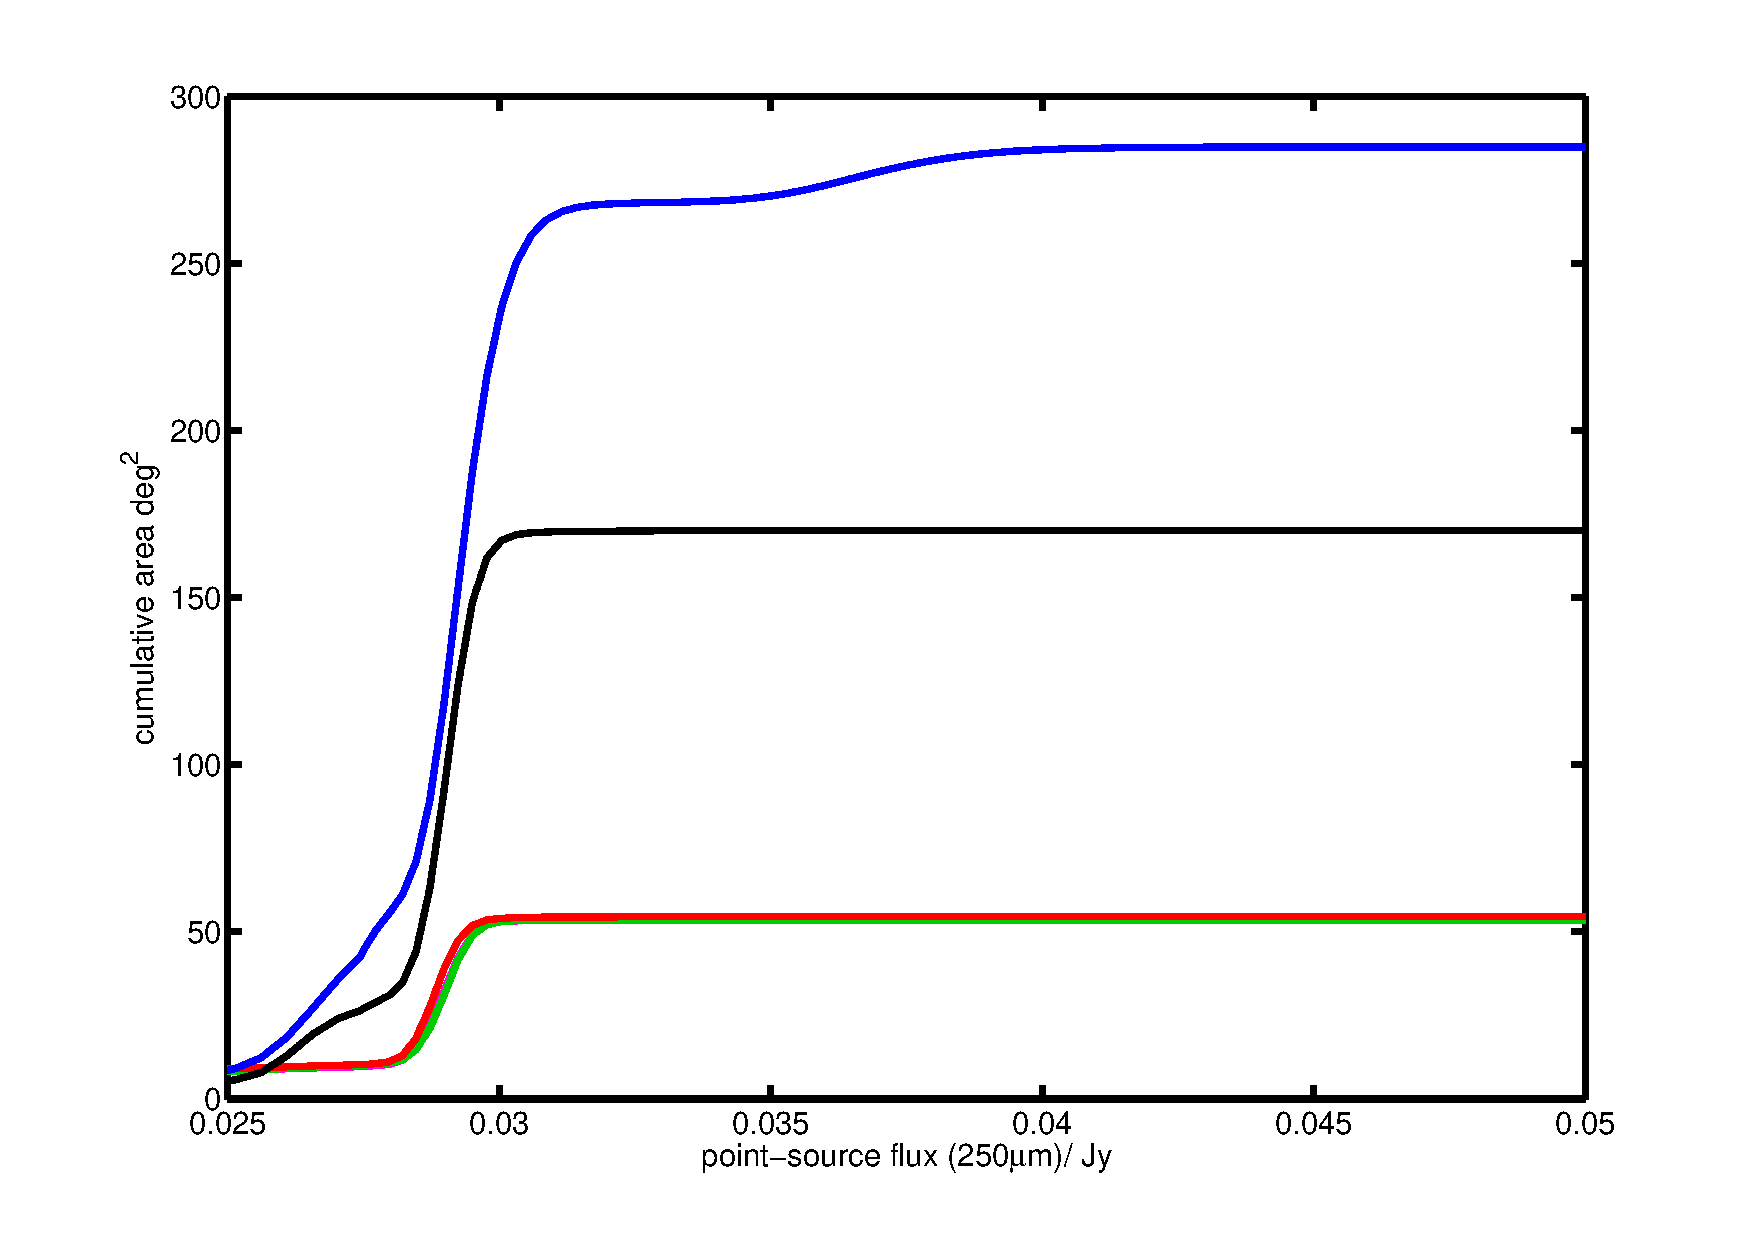
\includegraphics[width=0.5\textwidth]{flux_area_250.pdf}
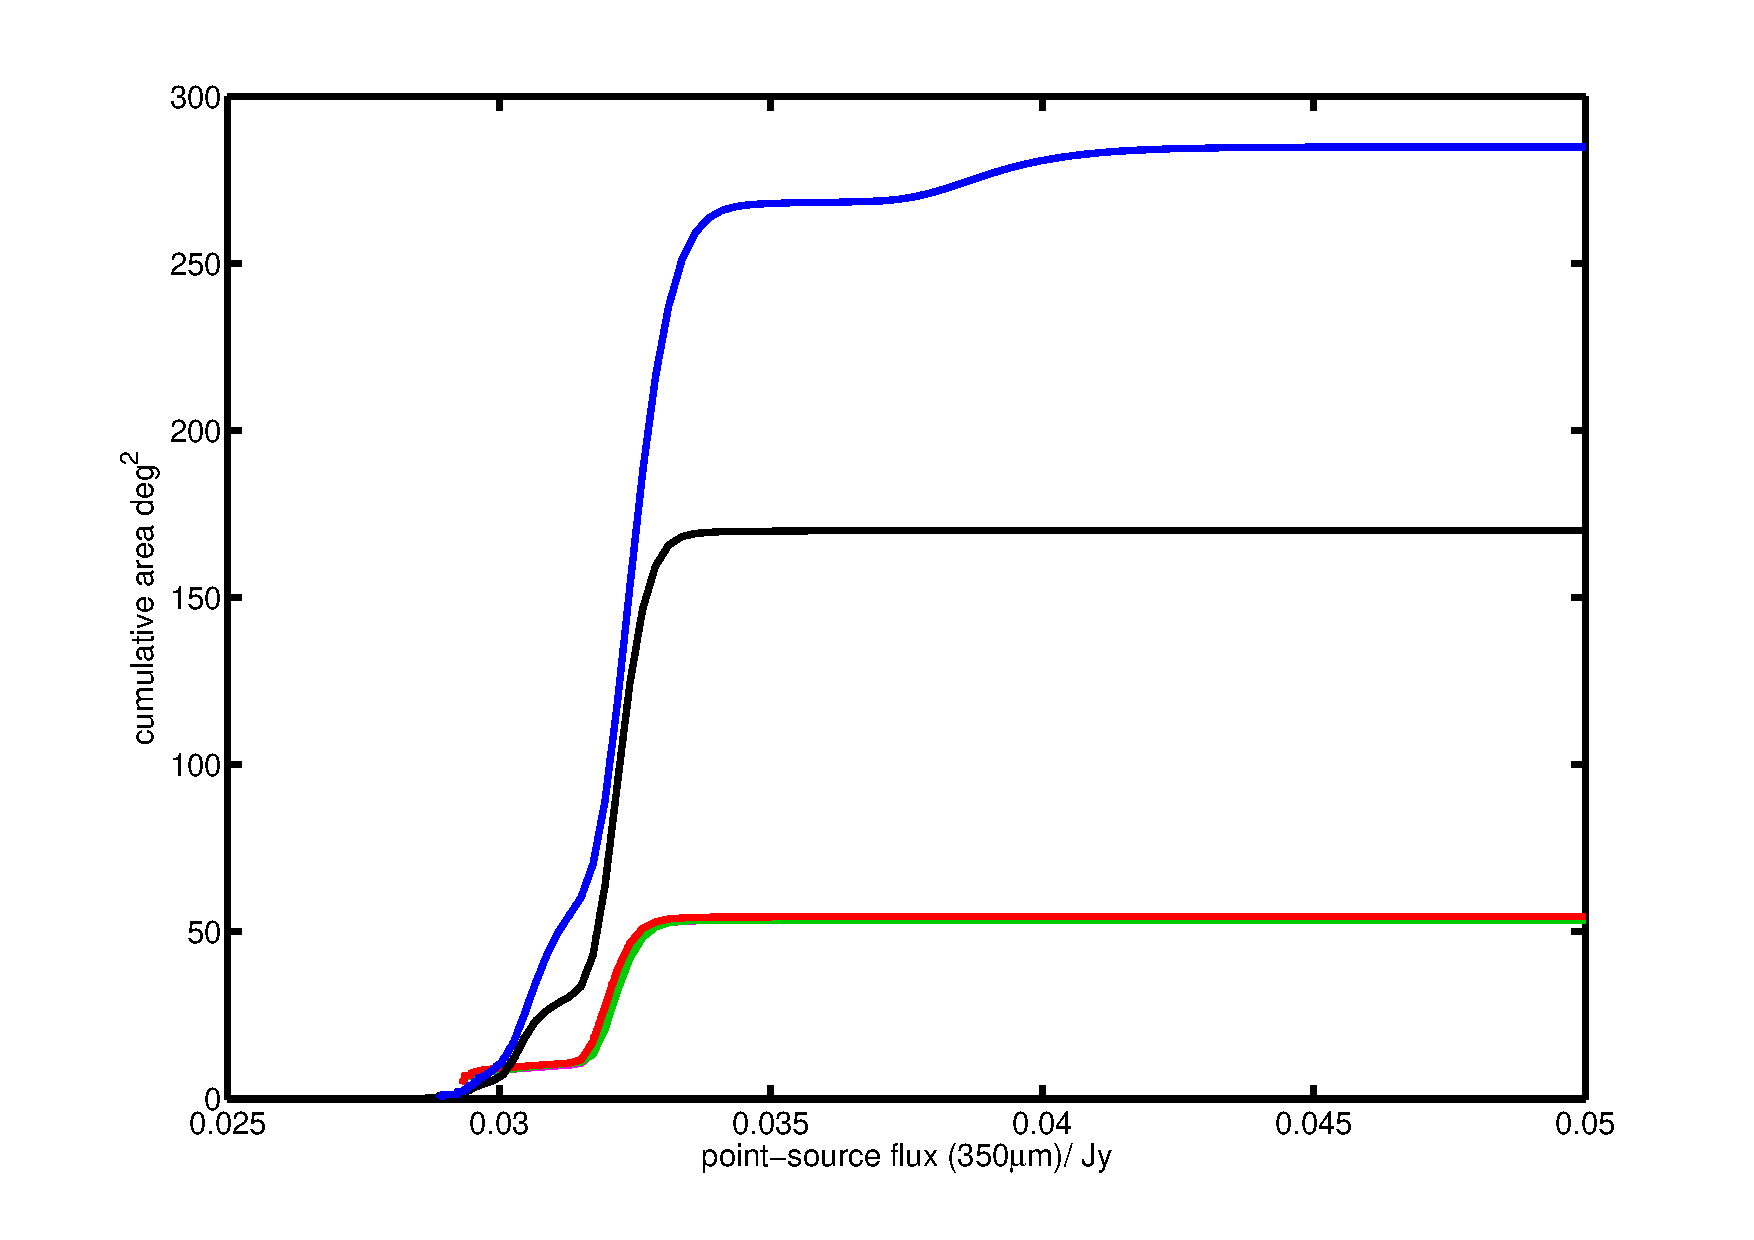
\includegraphics[width=0.5\textwidth]{flux_area_350.pdf}
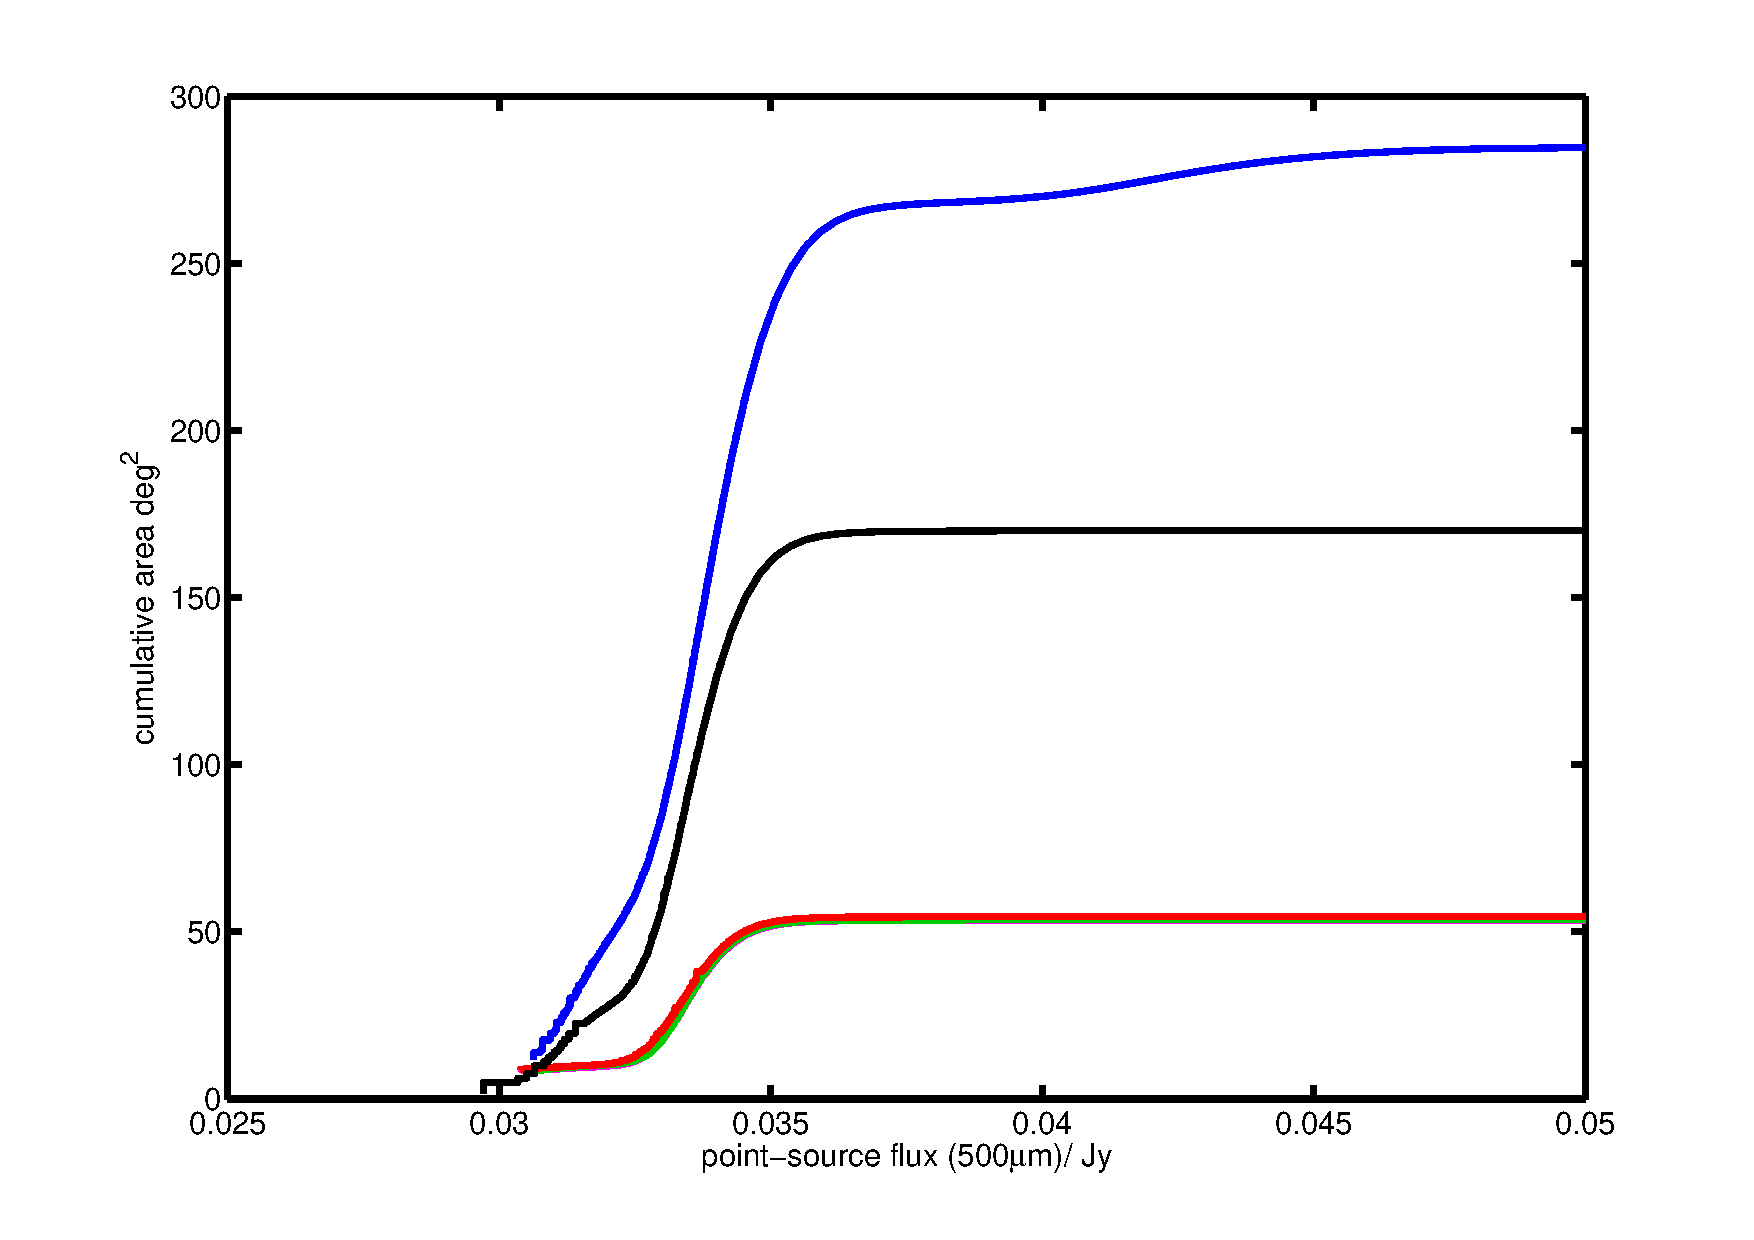
\includegraphics[width=0.5\textwidth]{flux_area_500.pdf}
\caption{The available survey area as a function of flux limit for the
  H-ATLAS fields: NGP black; SGP blue; GAMA9 magenta; GAMA12 green;
  and GAMA15 cyan.  The tile overlaps in each field provide deeper
  areas.  In the SGP, the most westerly tile was observed with only
  one observation for SPIRE, and has no cross-scan data. This means
  that $~6$\% of the area has a higher flux limit, $~40$mJy instead of
  the typical 28mJy for most of the survey. }

\label{fig_areas}
\end{figure}

\subsection{SPIRE point source flux uncertainties} 
Uncertainties on the flux measurements have been estimated using the
methods described in V16. The instrumental noise for each pixel in the
maps is estimated from the number of detector passes that contribute
to that pixel. The confusion noise was estimated by injecting fake
sources to the maps and measuring their fluxes in the same way as for
the real data. We found that the confusion noise varies as a function
of source flux, and we use a simple formula to approximate this:
\begin{equation} 
\sigma_{con250}^2 = \min(0.0049,f_{250}/5.6)^2 + 0.00253^2
\end{equation}

For the 350\mic and 500\mic band the confusion noise from the simulated
sources is roughly constant, $\sigma_{con350} = 0.00659$ and
$\sigma_{con500} = 0.00662$.

The instrumental noise varies over the maps, particularly in areas
which are covered by multiple tiles. This can be seen in the histogram
of the number of sources as a function of instrumental noise shown in
Figure~\ref{fig_noises}. This also shows the histogram of the number
of pixels as a function of noise, which is very similar to the
histogram of sources, as would be expected for sources roughly uniform
over the map.  The total noise is the result of adding the
instrumental and confusion noise in quadrature.

The peaks in the histogram of noises correspond to areas of different
coverage in the maps. The main peak is where there is coverage from
the 2-scan regions which have one pair of cross-scan tiles; the second
peak is from regions covered by three scans; then next from four scans
etc. (see Table 1 from S17).

%The slight offset is likely to be because pixels containing a
%source will be on average brighter than non-source pixels, and so will
%have a larger. 
The variation of noise across the maps means that the total area
available varies as a function of the 4 $\sigma$ flux limit
. Figure~\ref{fig_areas} shows the available area as a function of
flux for each of the H-ATLAS fields, including NGP, SGP and equatorial
GAMA fields.


%mf 250 11.3 mJy/beam
%mf 350 10.2 mJy/beam
%mf 500 9.4  mJy/beam

%in the SGP the std devs are
% 7.7 
% 7.0 
% 6.8 

The cumulative number of sources as a function of signal-to-noise in
the 250\mic detection band is shown in Fig.~\ref{fig_sn}.


\subsection{SPIRE extended source flux uncertainties} 
For extended sources where we have used an aperture flux estimate we
have estimated the noise from a Monte-Carlo analysis as described in
S17. For 2-scan regions the noise was found to depend on the radius of
the aperture as a double power-law, 

\begin{equation} 
  \sigma_{\mathrm{ap}}(\mathrm{mJy}) =
  \begin{cases} 
      Ar^\alpha &   \mathrm{if\ } r\le 50'' \\
      B(r-50)^\beta + A 50^\alpha & \mathrm{for\ } r>50'' 
    \end{cases}
\end{equation} 

The constants $A$, $B$, $\alpha$, and $\beta$  are given in Table~3 of S17. 
For regions covered by more than two scans, the instrumental noise contribution
decreases as shown in Table1 of S17, and the change is subtracted in
quadrature as shown in Equation~6 of S17. 

\subsection{PACS flux uncertainties} 

Our PACS photometry is all based on aperture measurements, so the same
approach is used for both point-sources and extended sources. As for
SPIRE we estimate the uncertainty of the fluxes by considering random
apertures the same size as the point-source apertures. We place three
thousand apertures randomly over the 2-scan regions of the maps and
calculate summed flux in each; then use the standard deviation of the
random aperture sums to provide the one sigma uncertainty estimate. We
used radii ranging from the beam FWHM to 100'' and found a good fit to
the radius dependence is given by a double power law as used for the
SPIRE. The values of the constants $A$, $B$, $\alpha$, and $\beta$ are
given in Table~3 of S17. The noise expected for areas covered by more
than 2 scans is calculated by assuming that the instrumental noise
scales as $1/\sqrt{N_{\mathrm{scan}}}$, as shown in Equation~8 of
S17. 

\subsection{The distribution of signal to noise ratios} 

The cumulative distribution of the number of sources as a function of
signal to noise for eall five fields and all five bands is shown in
Figure~\ref{fig_sn}. The three GAMA fields have similar areas and so
have fewer sources in total compared to the NGP and SGP. At the very high
signal-to-noise end of the distributions the small number of sources
lead to large Poisson errors and large Cosmic variance between the
fields, but the overall
distribution of noises is very similar between the fields, and so the
general shapes of the distributions are very similar. 

\begin{figure}
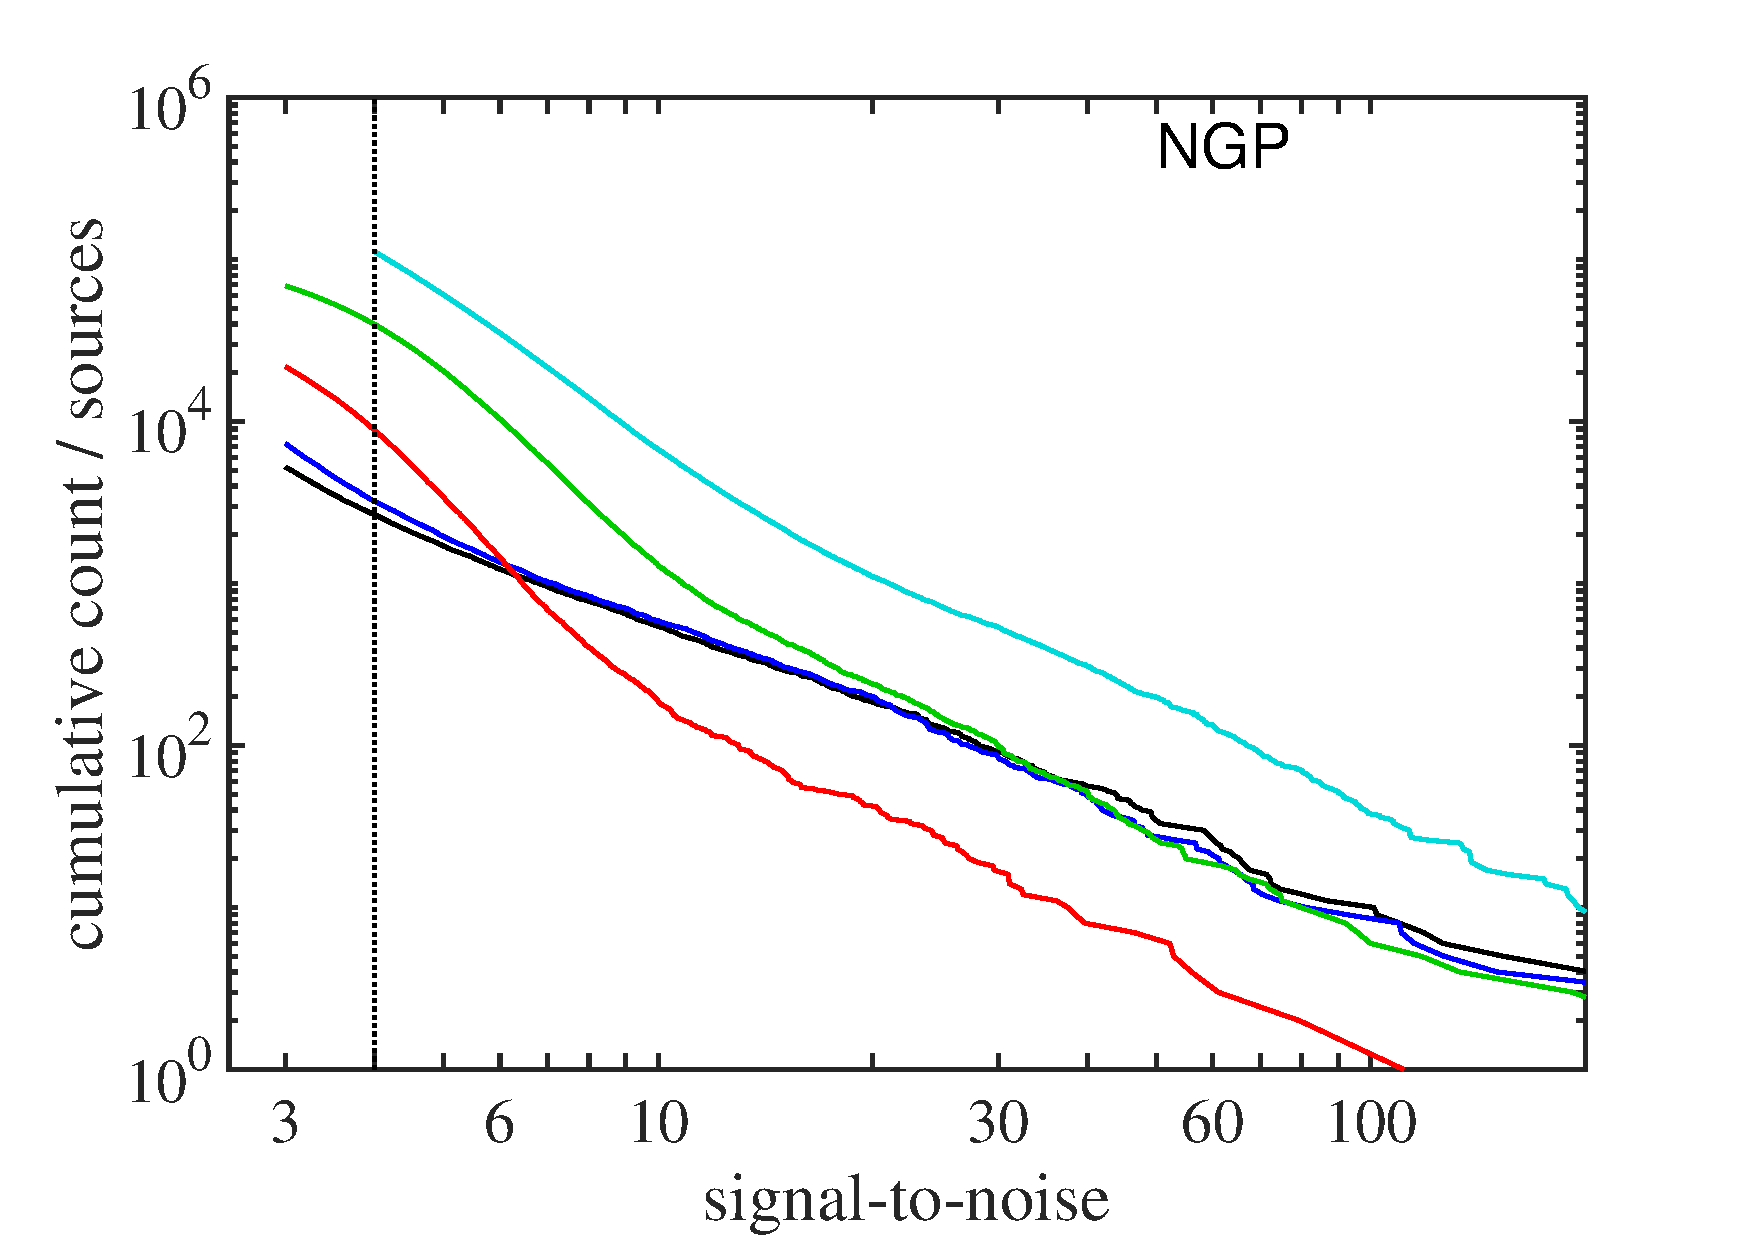
\includegraphics[width=0.5\textwidth]{cum_sn_NGP.pdf}
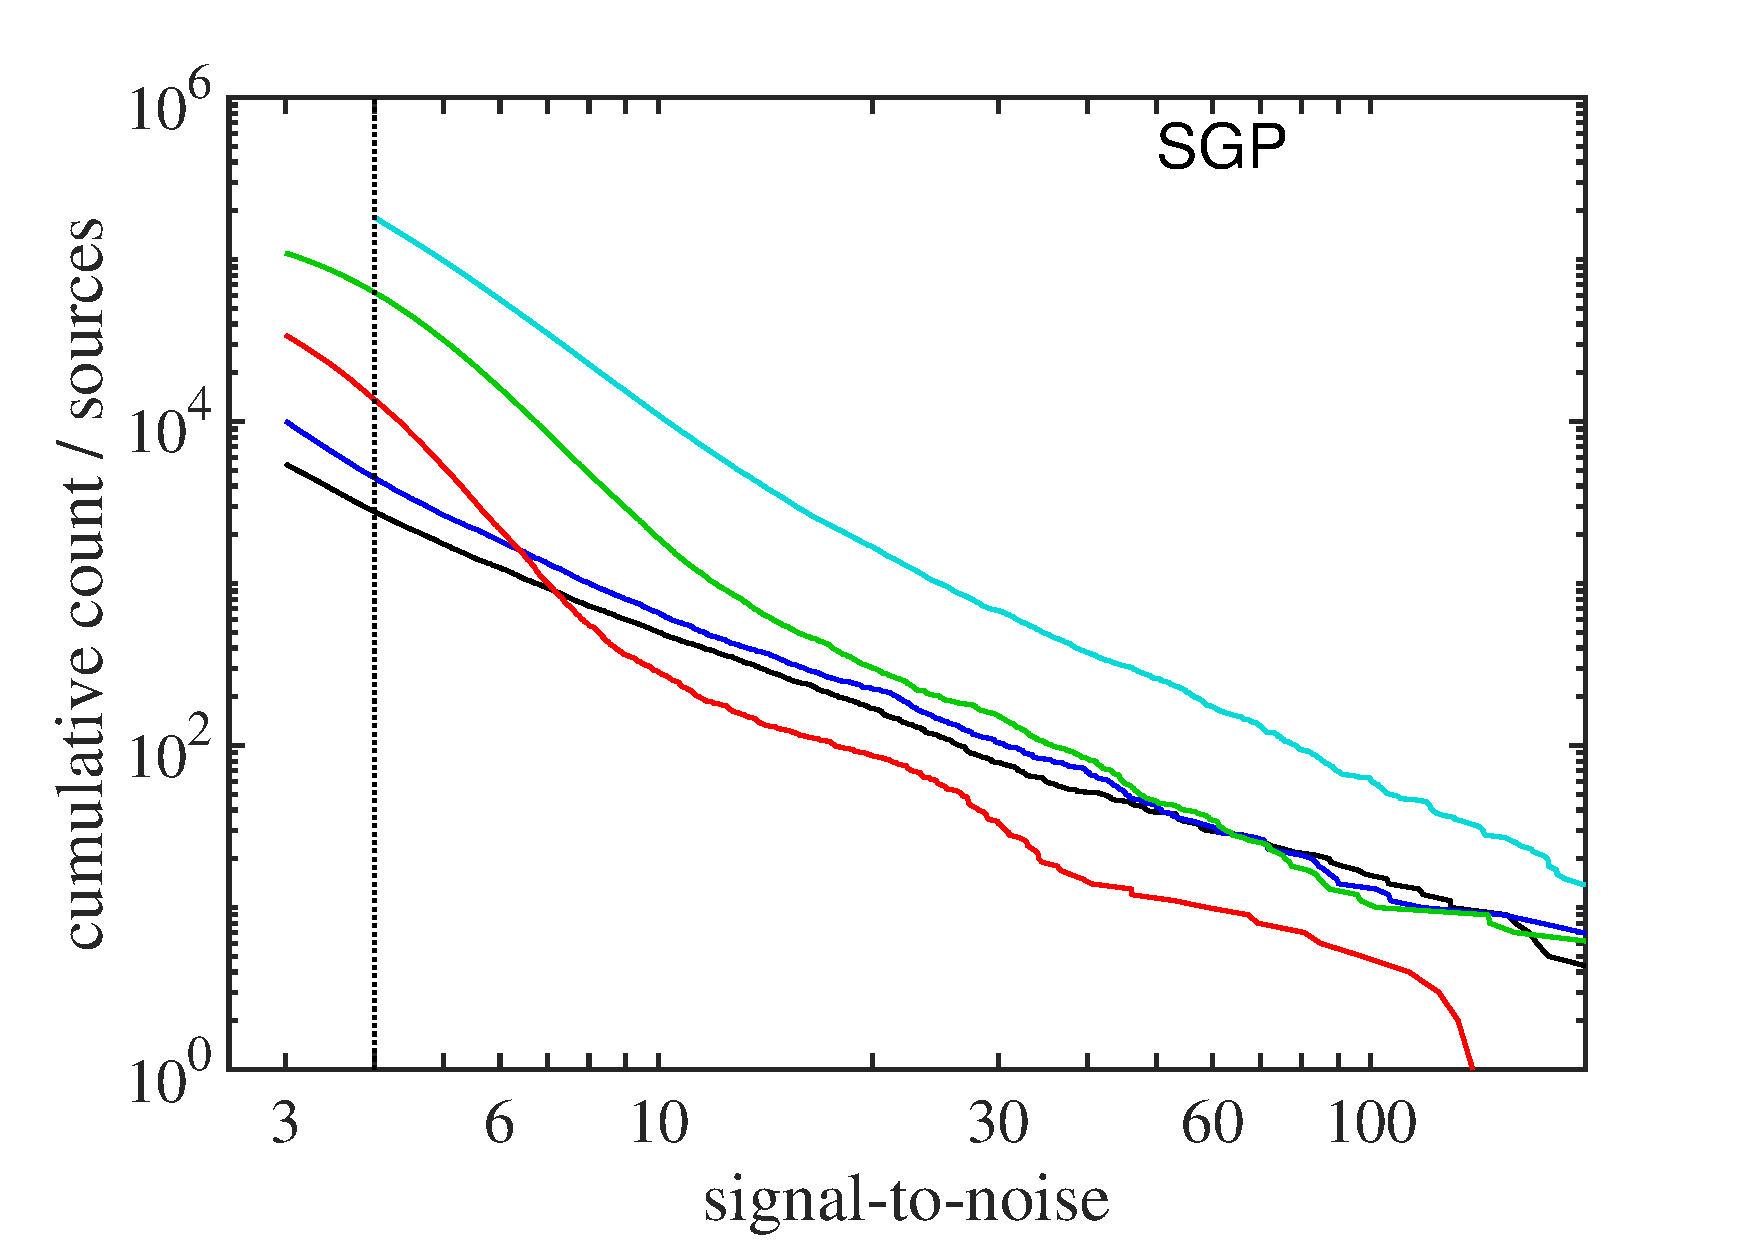
\includegraphics[width=0.5\textwidth]{cum_sn_SGP.pdf}
 \caption{\protect\label{fig_sn} The cumulative number of sources as a function
   of signal-to-noise at 100\mic (black), 160\mic (blue), 250\mic (cyan),
  350\mic (green) and 500\mic (red). The NGP area is shown in the top panel,
  and the SGP in bottom panel. The vertical dotted line shows the
  4-$\sigma$ limit. 
} 
\end{figure}
% \begin{figure}
% 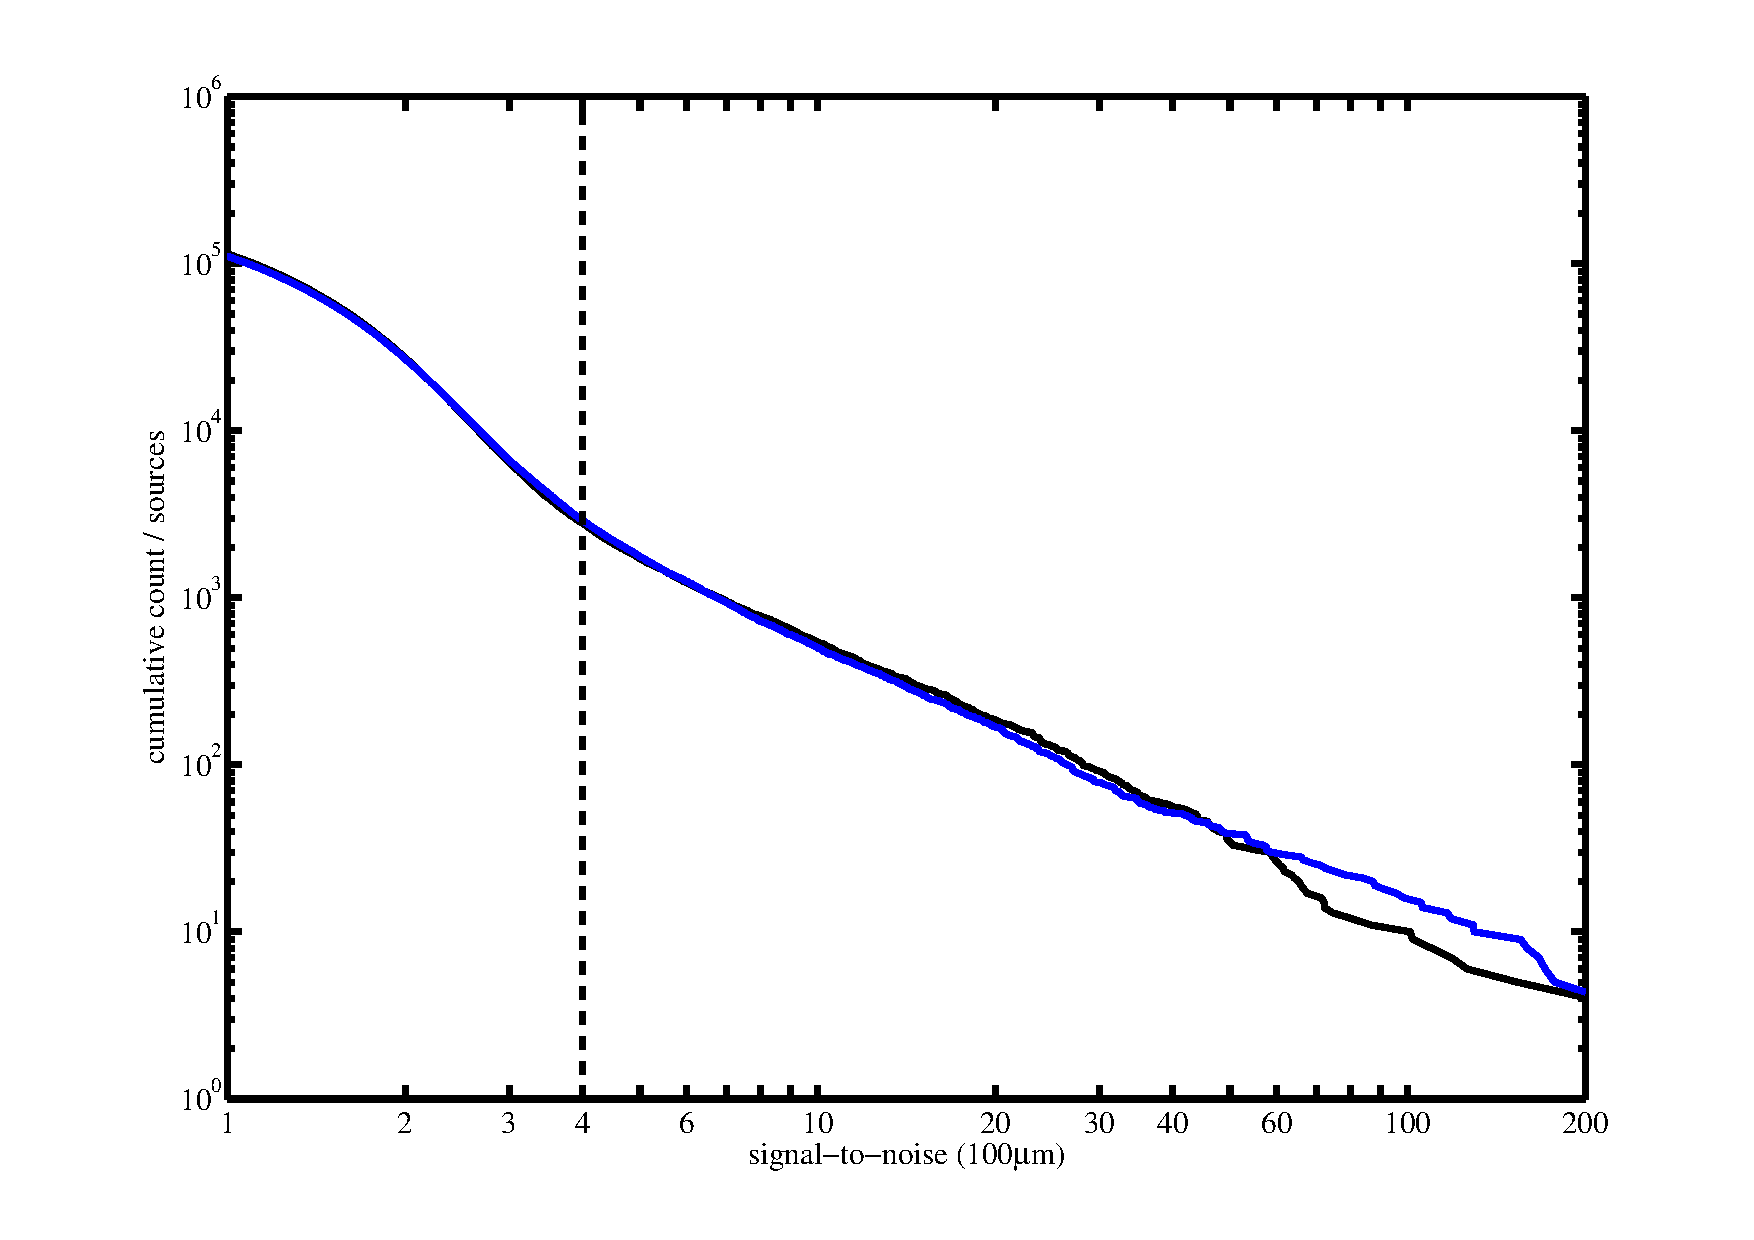
\includegraphics[width=0.42\textwidth,clip,trim={0 9mm 0mm 16mm}]{cum_sn_100.pdf}
% 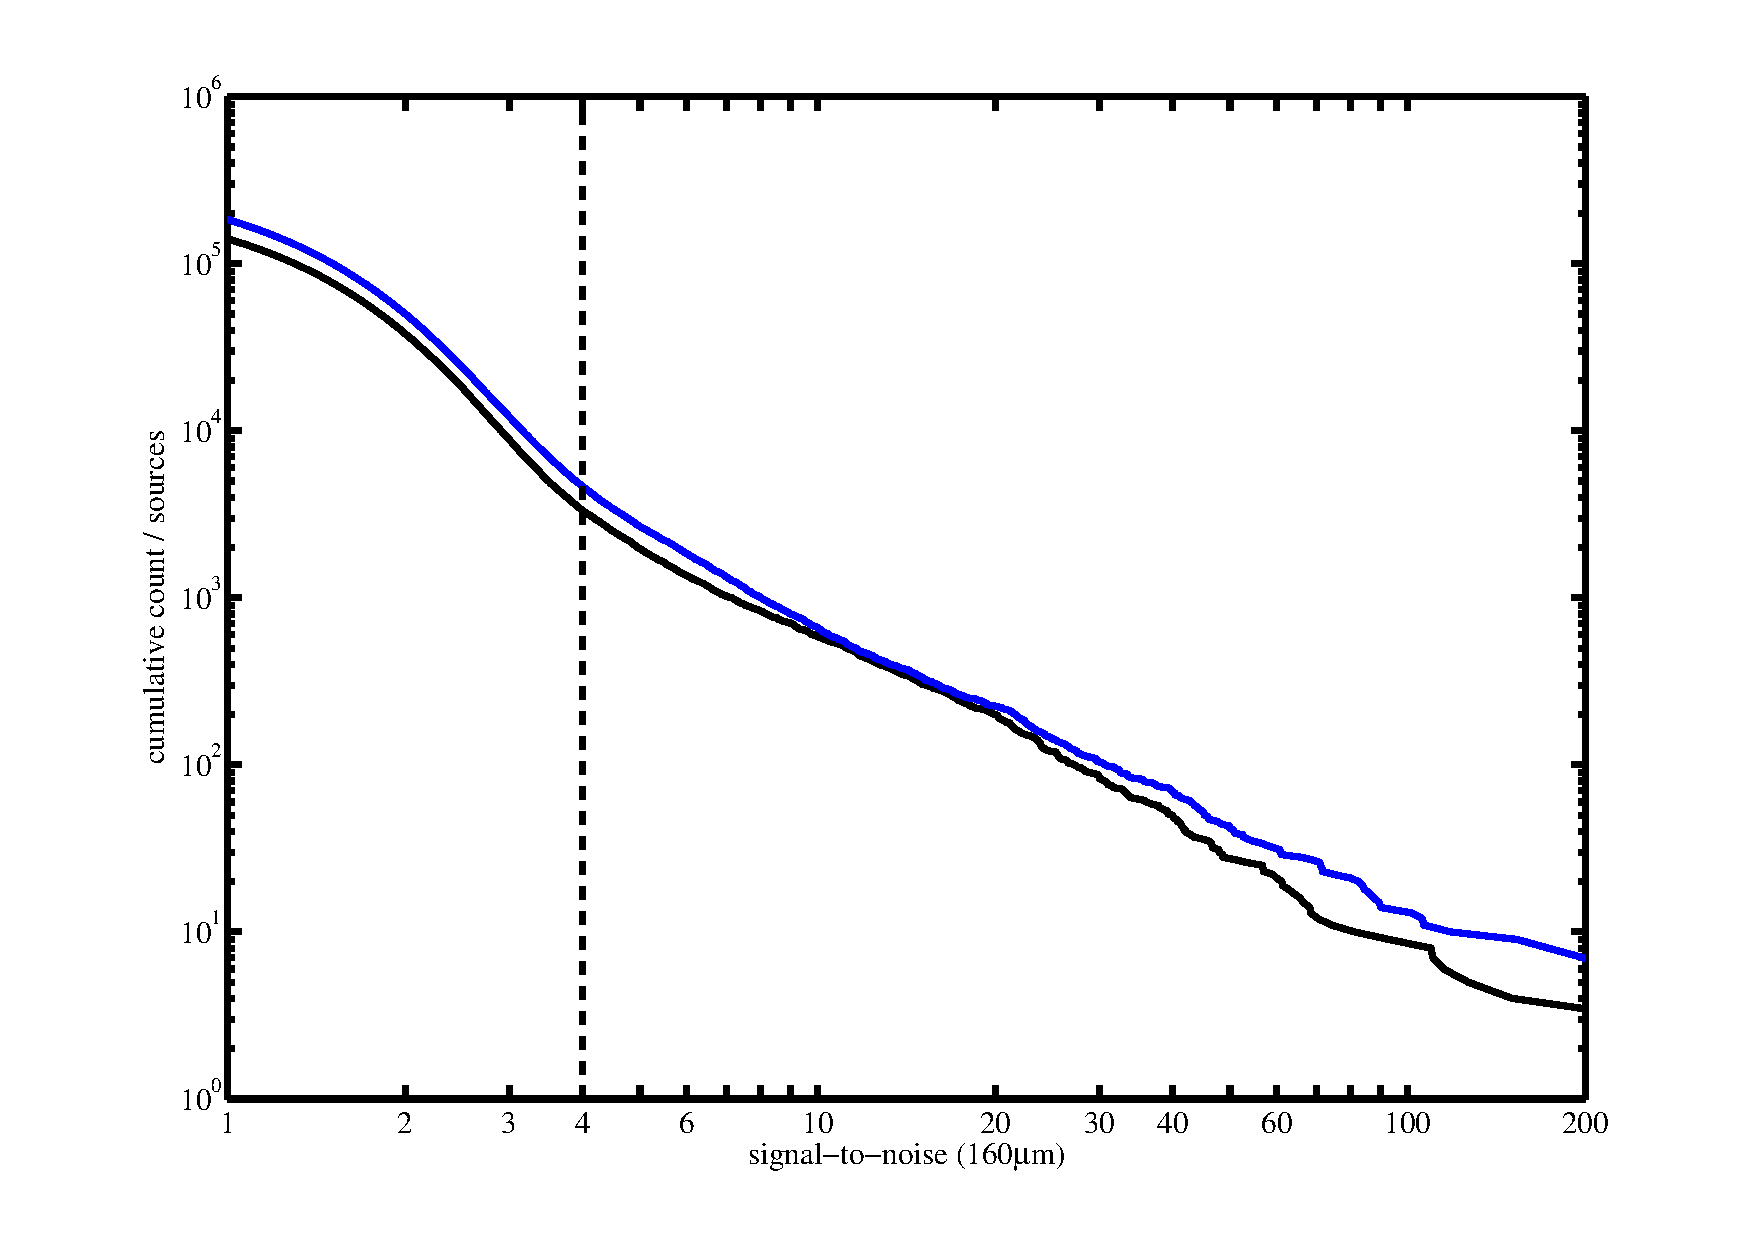
\includegraphics[width=0.42\textwidth,clip,trim={0 9mm 0mm 16mm}]{cum_sn_160.pdf}
% 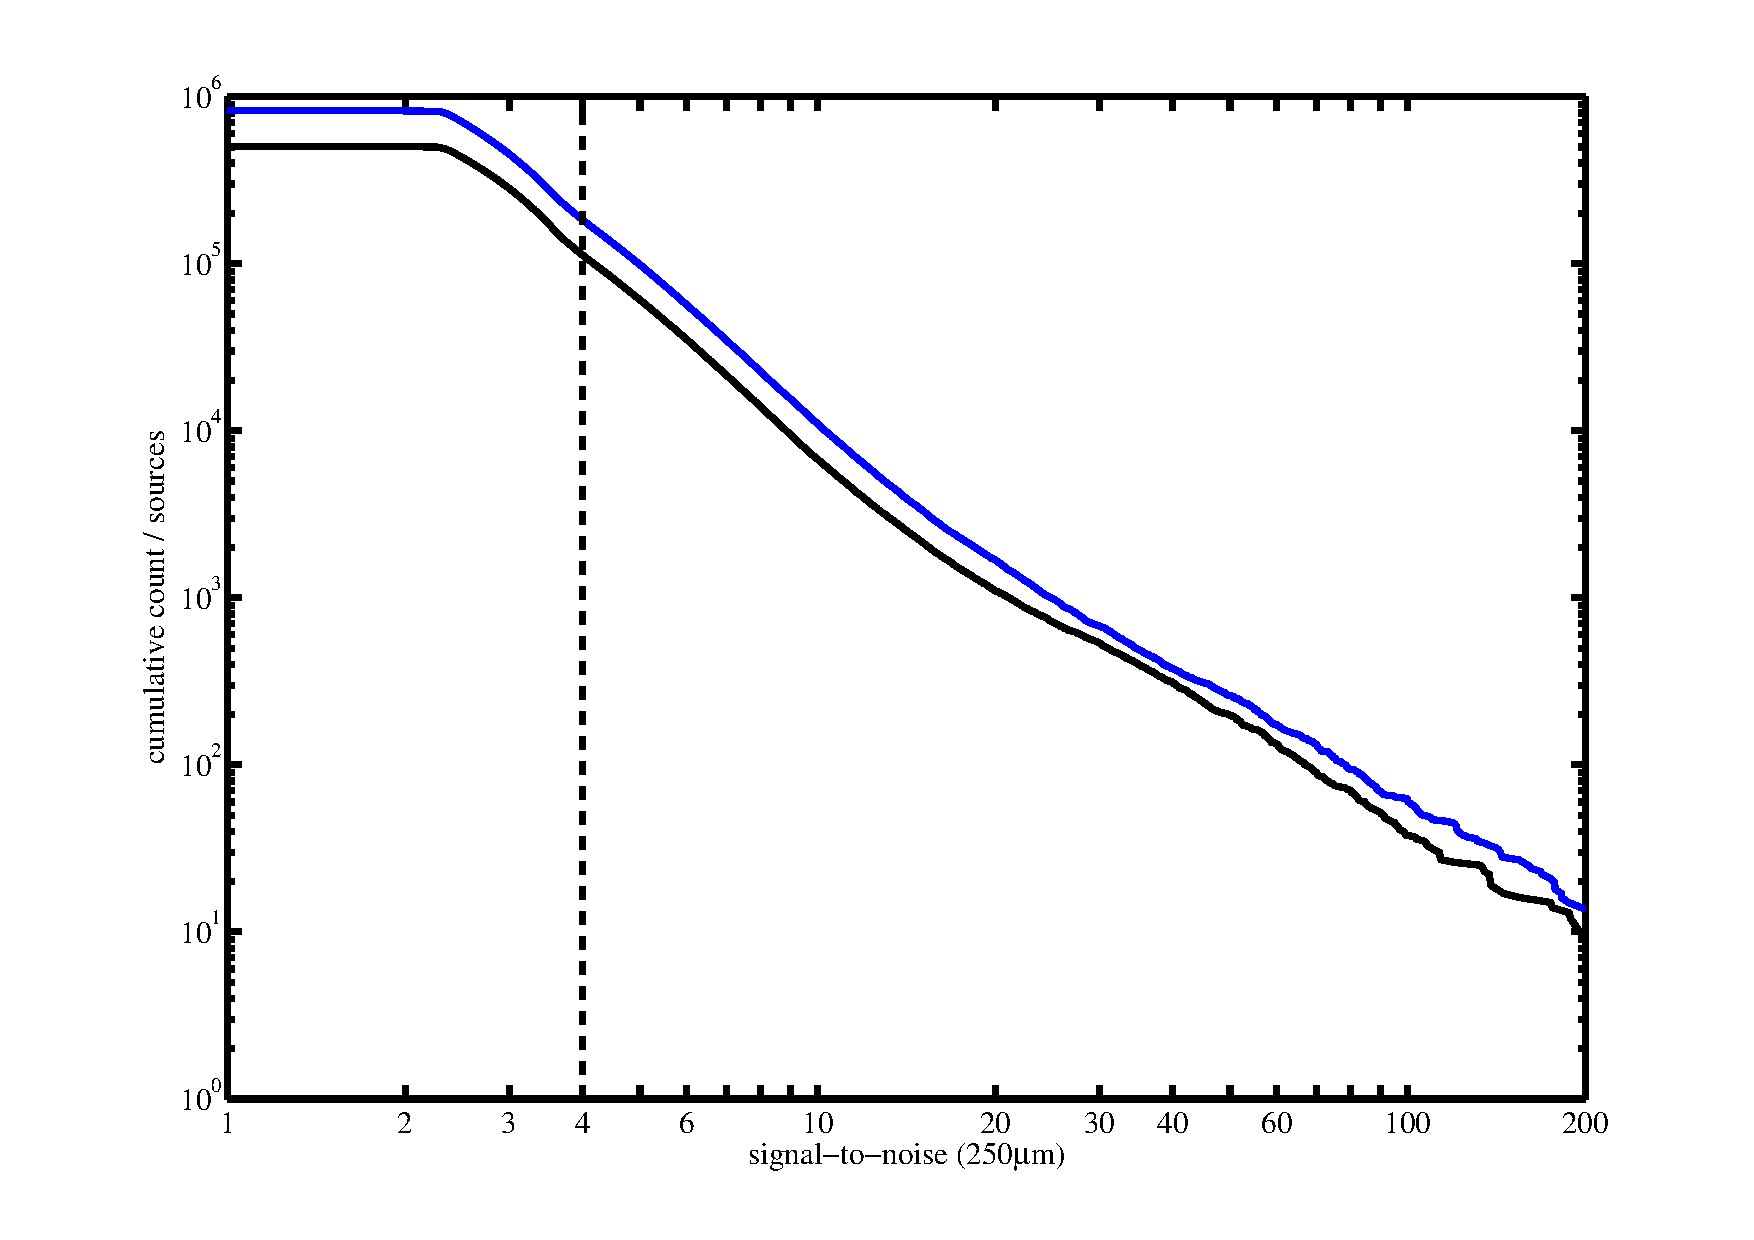
\includegraphics[width=0.42\textwidth,clip,trim={0 9mm 0mm 16mm}]{cum_sn_250.pdf}
% 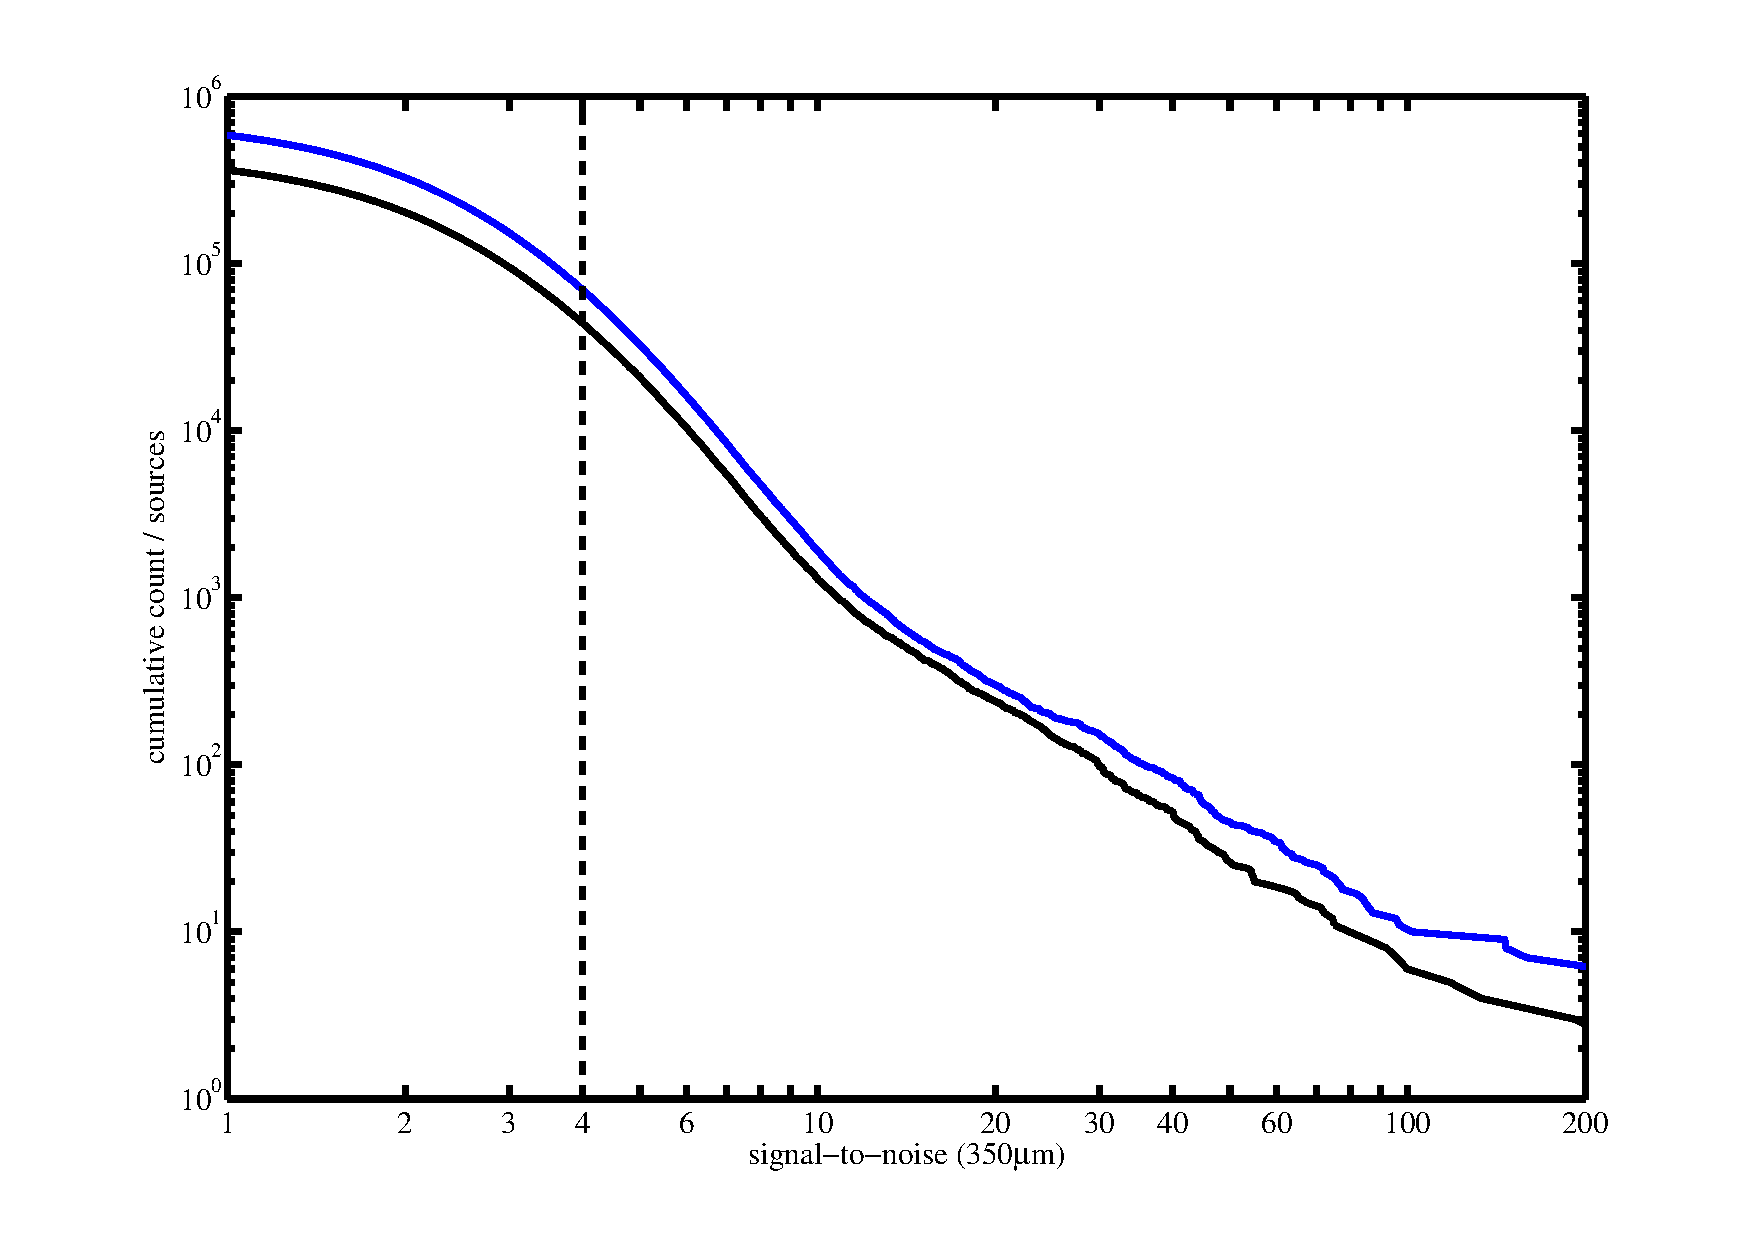
\includegraphics[width=0.42\textwidth,clip,trim={0 9mm 0mm 16mm}]{cum_sn_350.pdf}
% 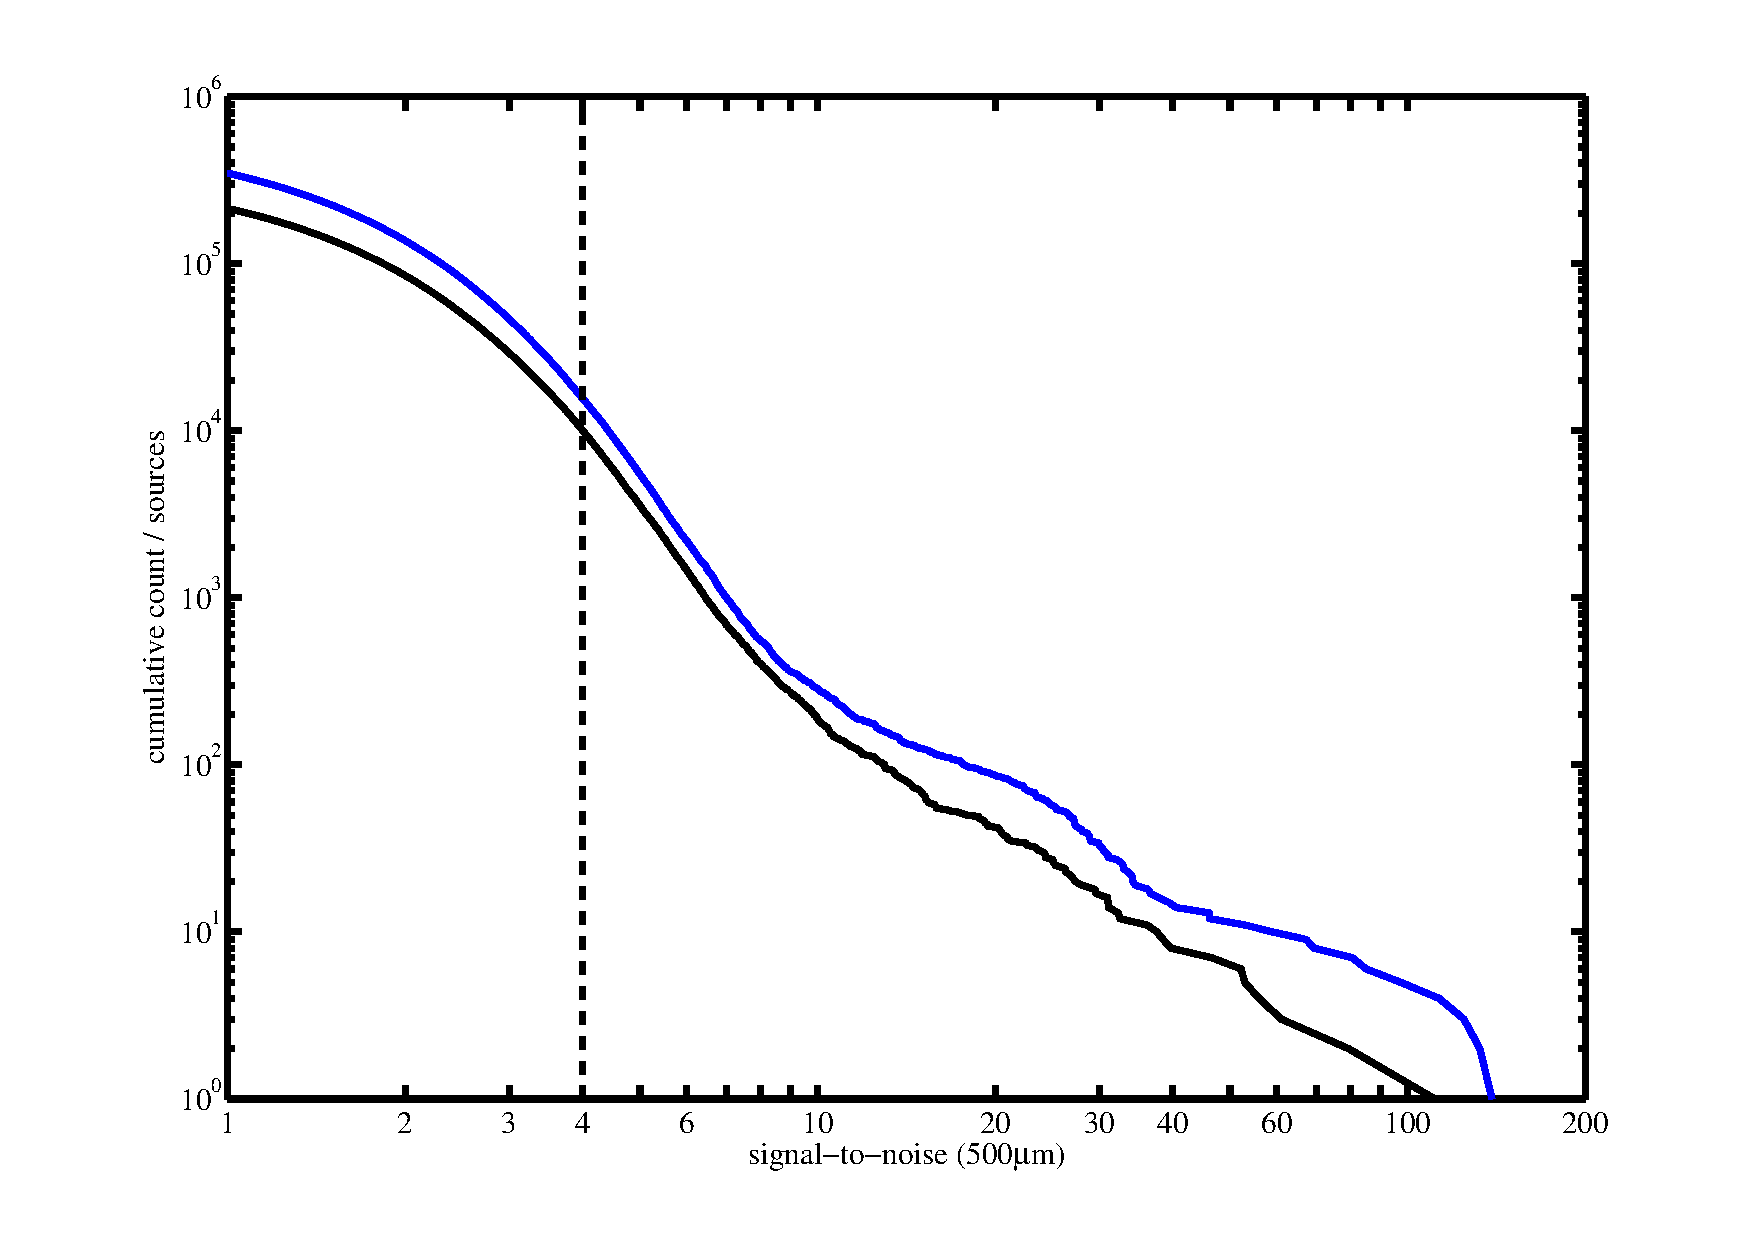
\includegraphics[width=0.42\textwidth,clip,trim={0 9mm 0mm 16mm}]{cum_sn_500.pdf}
%  \caption{\protect\label{fig_sn} The cumulative number of sources as a function
%    of signal-to-noise at  100\mic, 160\mic, 2250\mic, 350\mic and 500\mic} 
% \end{figure}

\section{Positional uncertainty} 

Astrometry for the SPIRE maps is calibrated by comparing preliminary
source catalogues to SDSS galaxies in the NGP and VST ATLAS in the SGP
(see S17). The final source catalogues are thus calibrated to the SDSS
and VST astrometric frame. The positional error distribution for the
NGP catalogue has been estimated as part of our optical ID process
(F17). The distribution of positional offsets is fitted by the
expected clustering of galaxies around the FIR galaxies convolved by a
Gaussian error distribution. We find that the positional error,
$\sigma_\mathrm{pos}$, varies from 1.2'' to 2.4'' as the
signal-to-noise in flux varies from 10 to 5, so $\sigma_\mathrm{pos} =
2.4 (\mathrm{SNR}/5)^{-0.84}$.

These values of positional uncertainty are consistent with the
positional errors found in the recovered positions of sources in our
simulations (V16). 


%\begin{figure}
%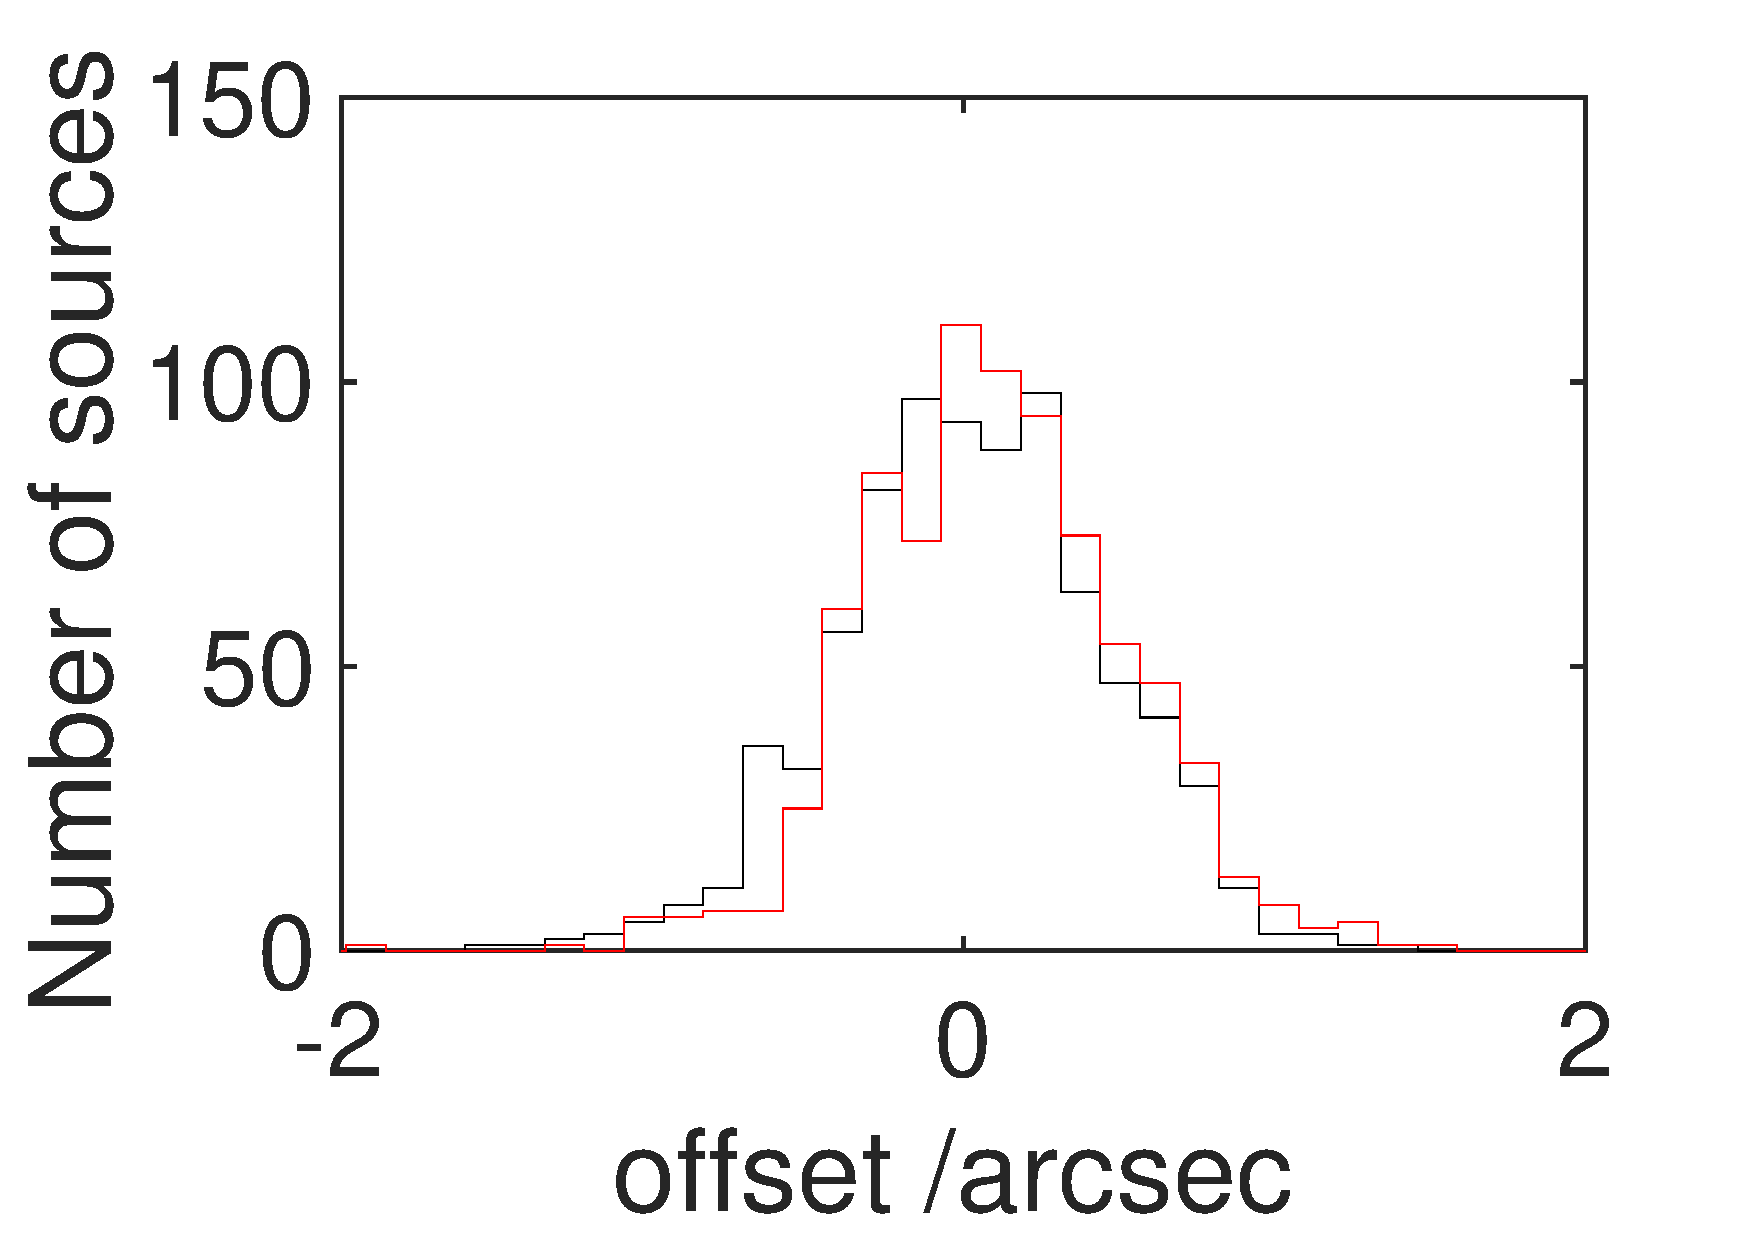
\includegraphics[scale=0.3]{ngp_pos_err_hist.pdf}
%\caption{\protect\label{fig_pos_err_hist} The distribution of
%  positional offsets between SPIRE and SDSS sources in the NGP. 
%The black histogram shows the offsets in RA, and the red line the
%offsets in DEC. 
%!!!IS this the map alignment histogram or the XID one? Which sources are included?
%}
%\end{figure}


The mean positional errors as a function of position within the NGP
and SGP fields are shown in Fig.~\ref{fig_pos_errs}. Though there are
hints of systematic variations in different part of the field, they
are typically around the arcsecond level, as expected from the
pointing error of the Herschel satellite. 

\begin{figure*}
%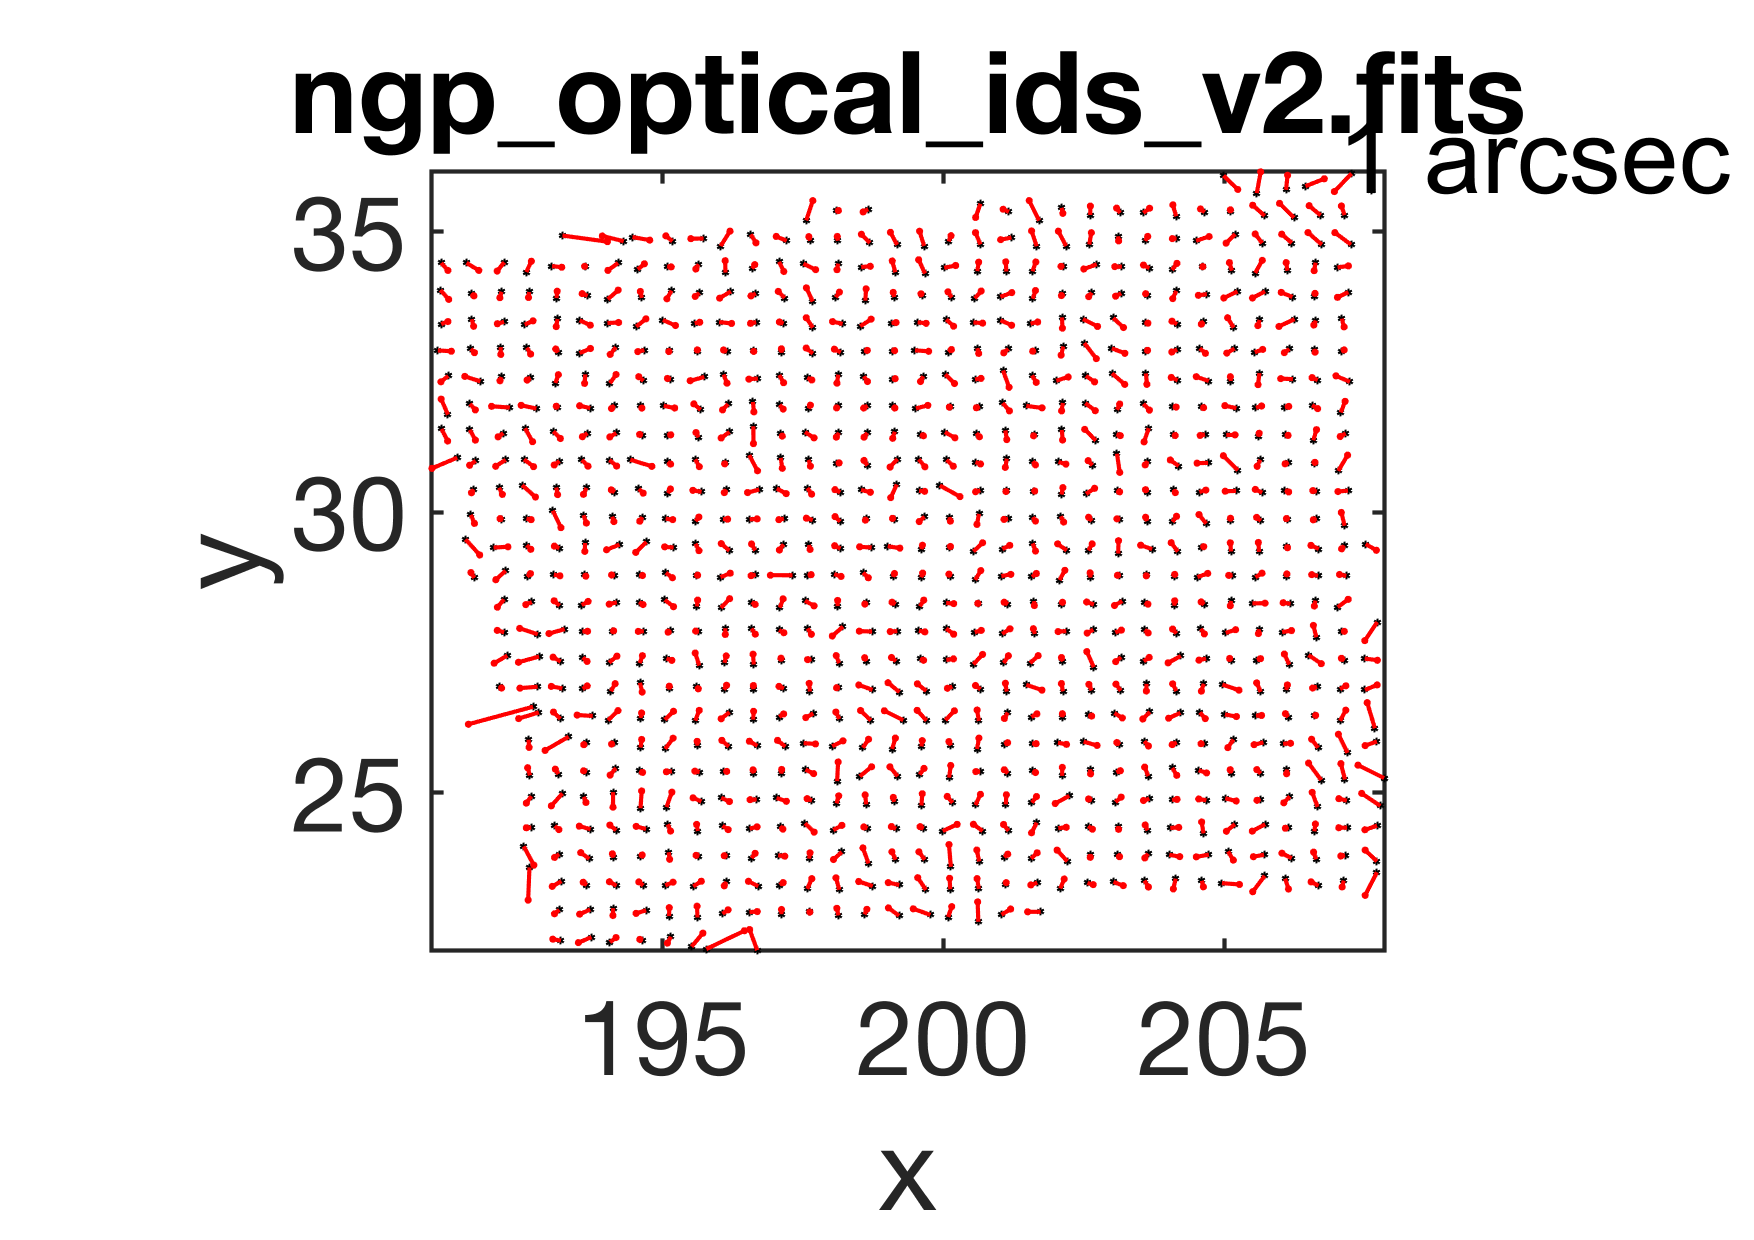
\includegraphics[scale=0.3]{ngp_posn_errors_new.pdf}
%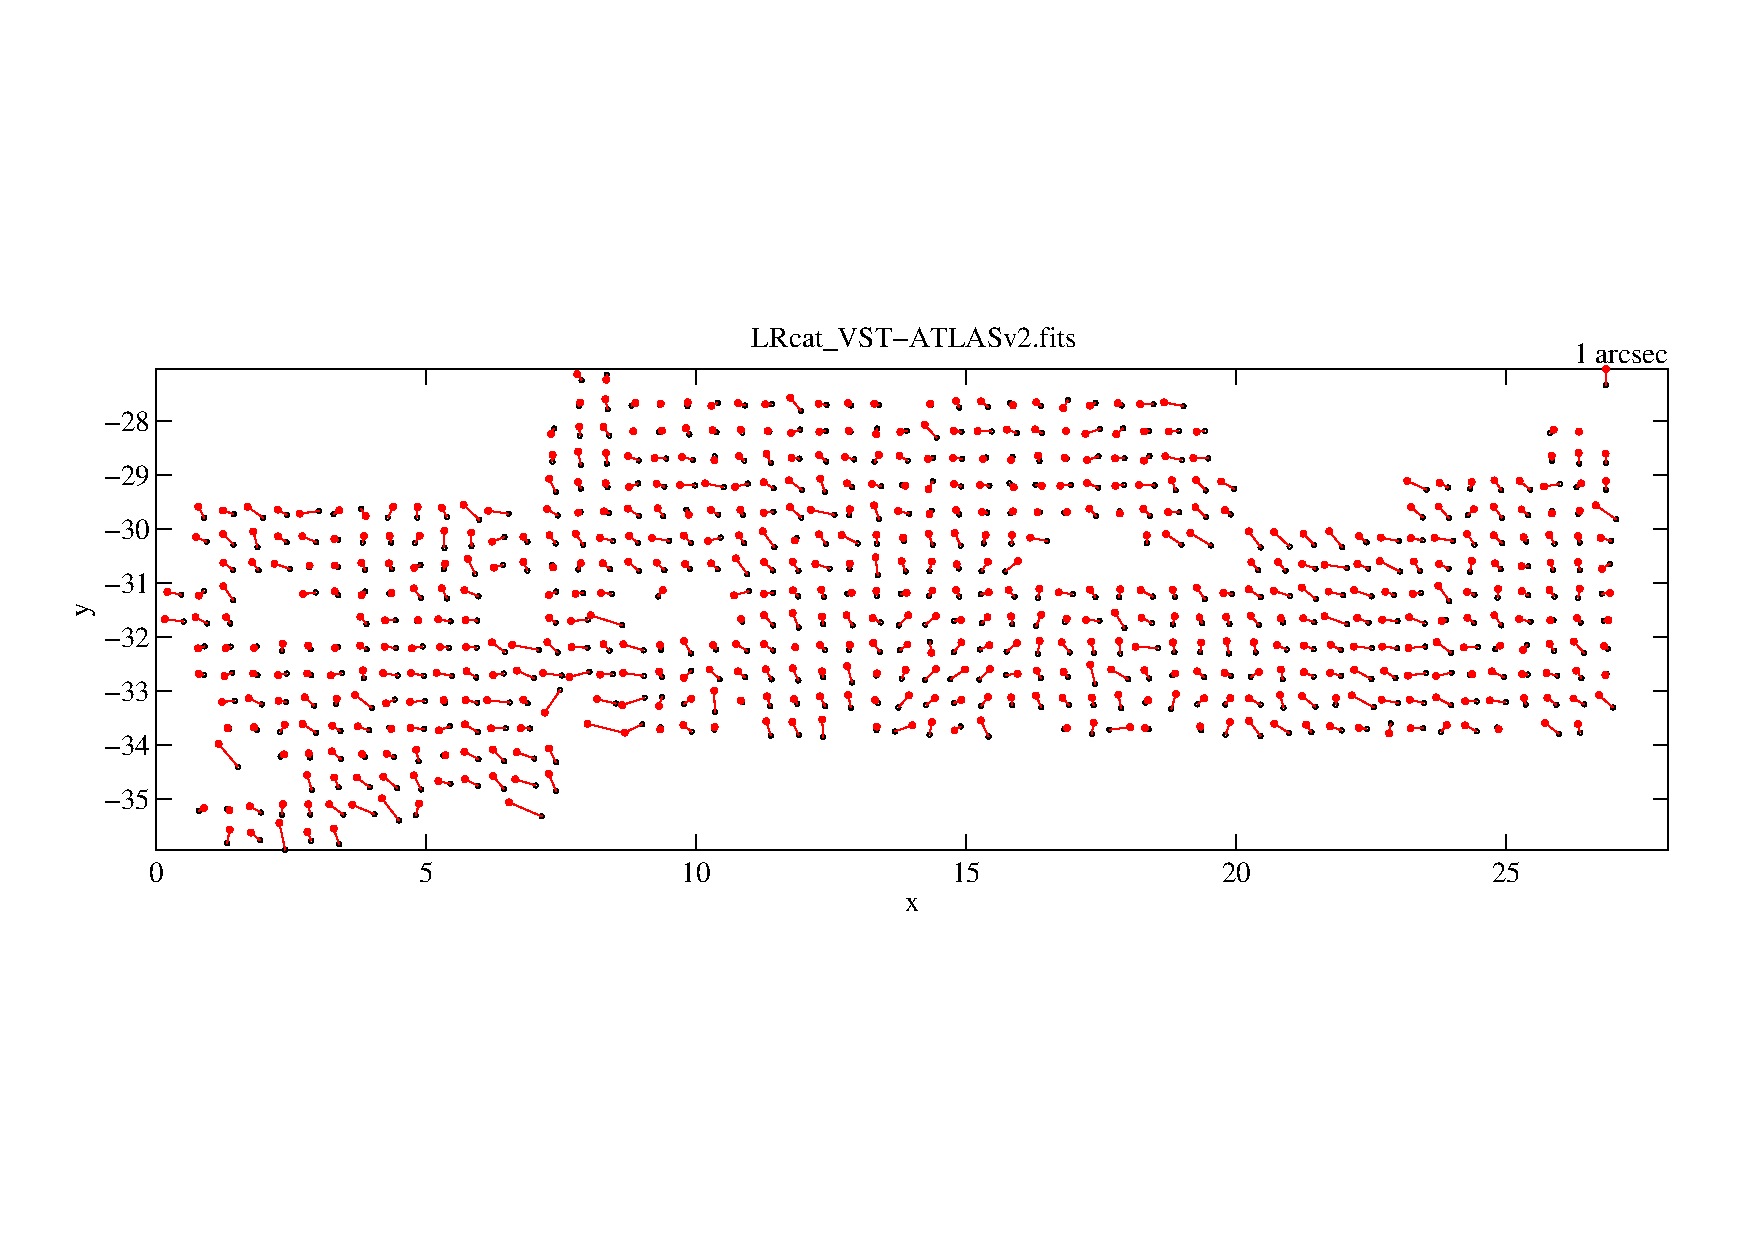
\includegraphics[scale=0.3,trim=0 45mm 0mm 45mm]{sgp_astrometry2.pdf}
%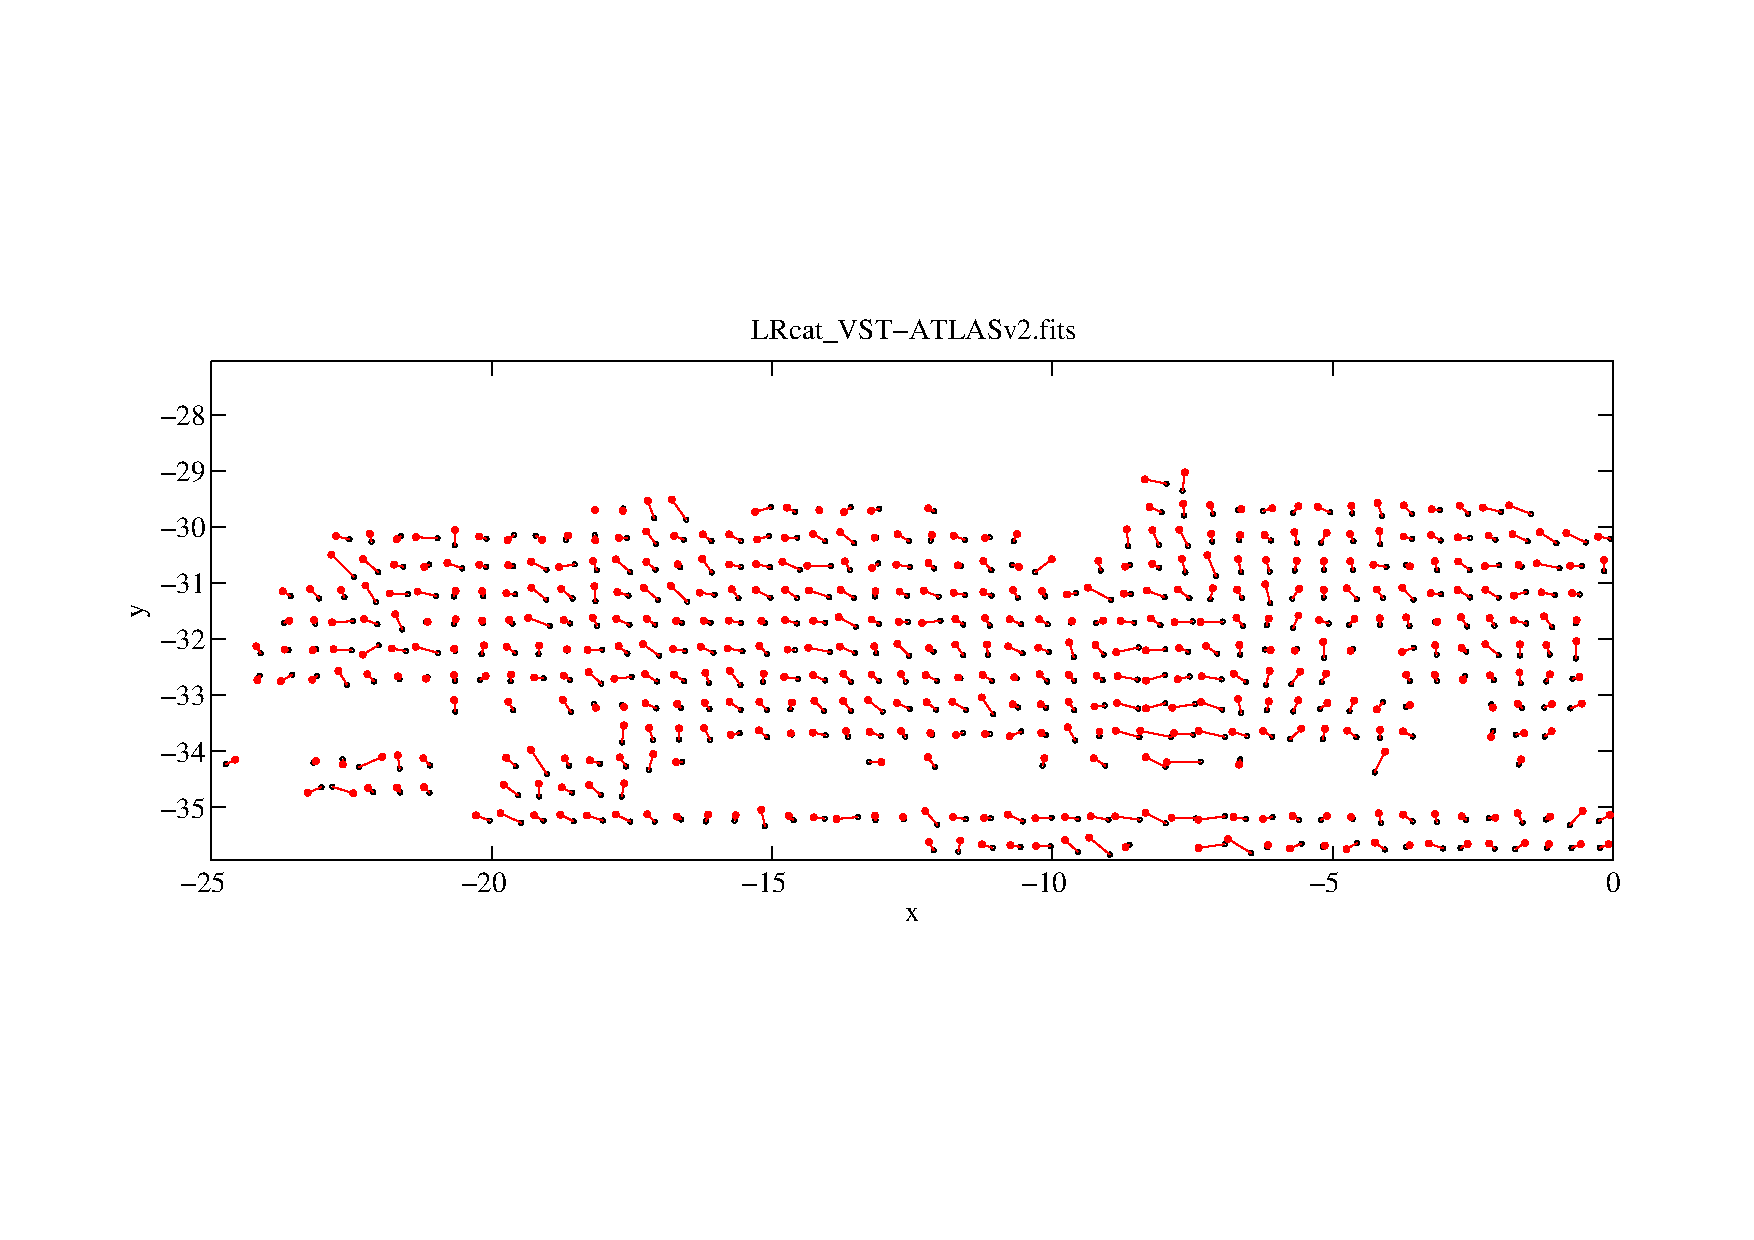
\includegraphics[scale=0.3,trim=0 45mm 0mm 45mm]{sgp_astrometry1.pdf}
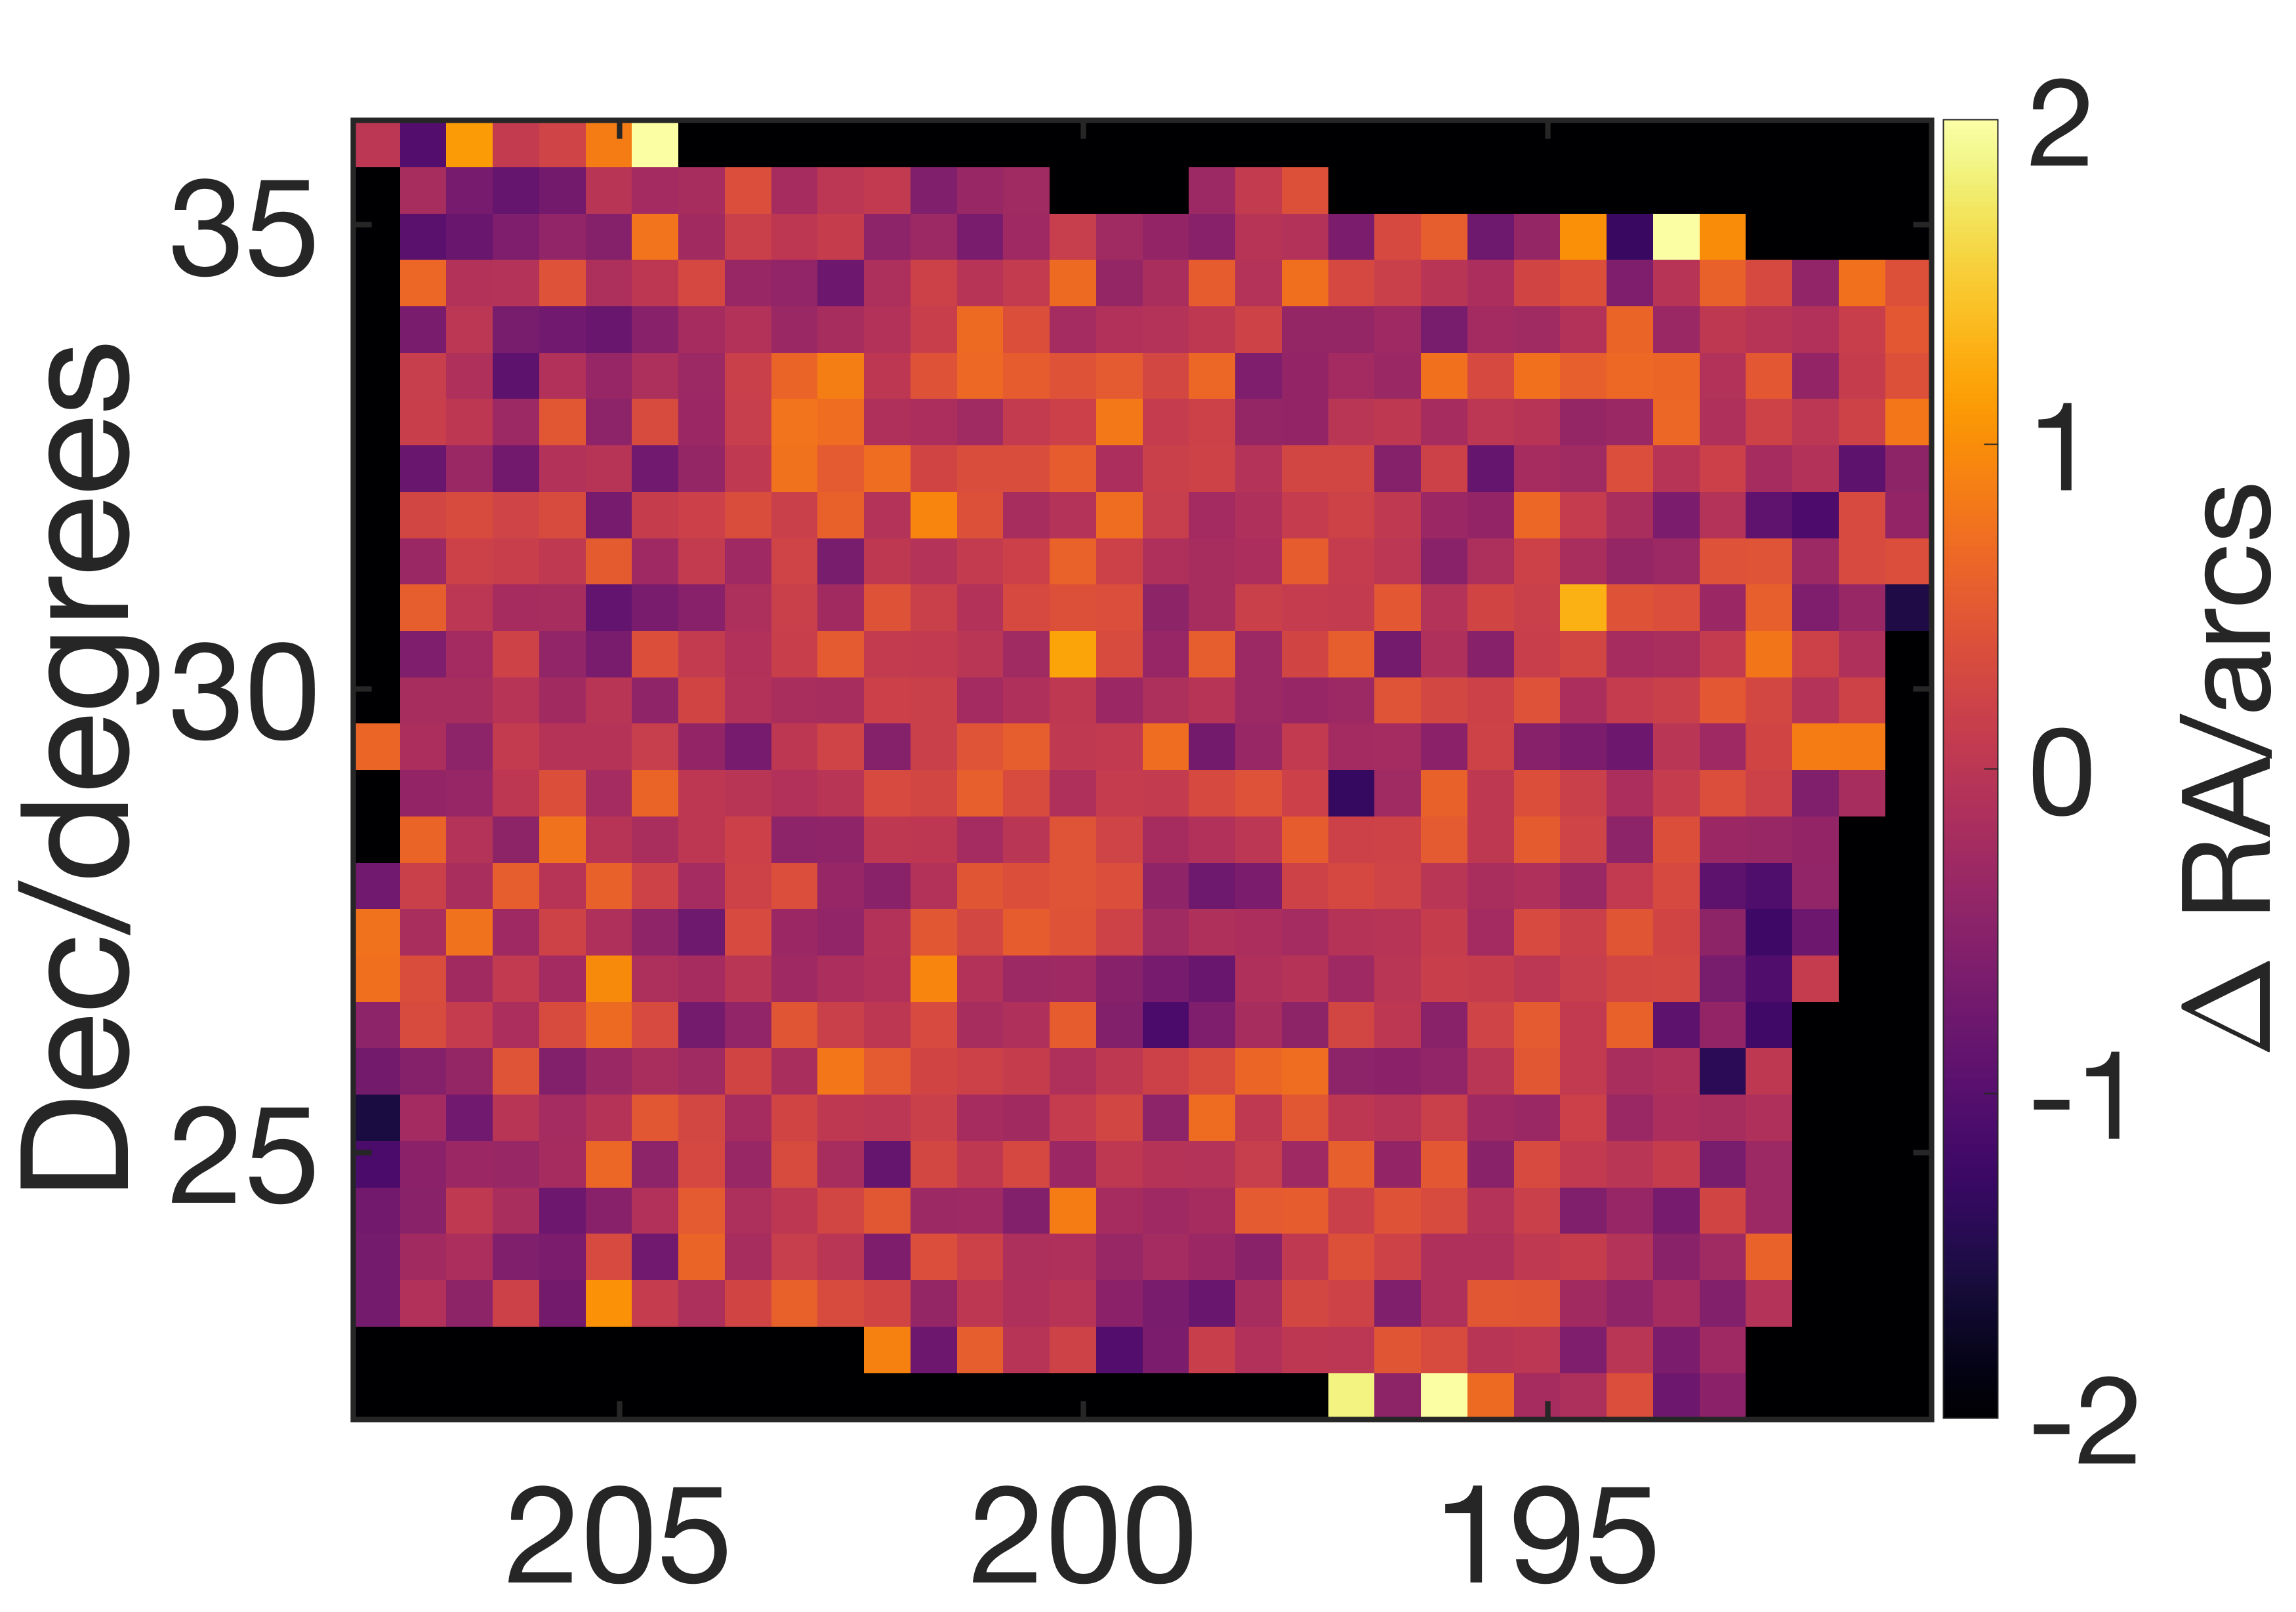
\includegraphics[scale=0.23]{ngp_dra.png} \hspace{5mm}
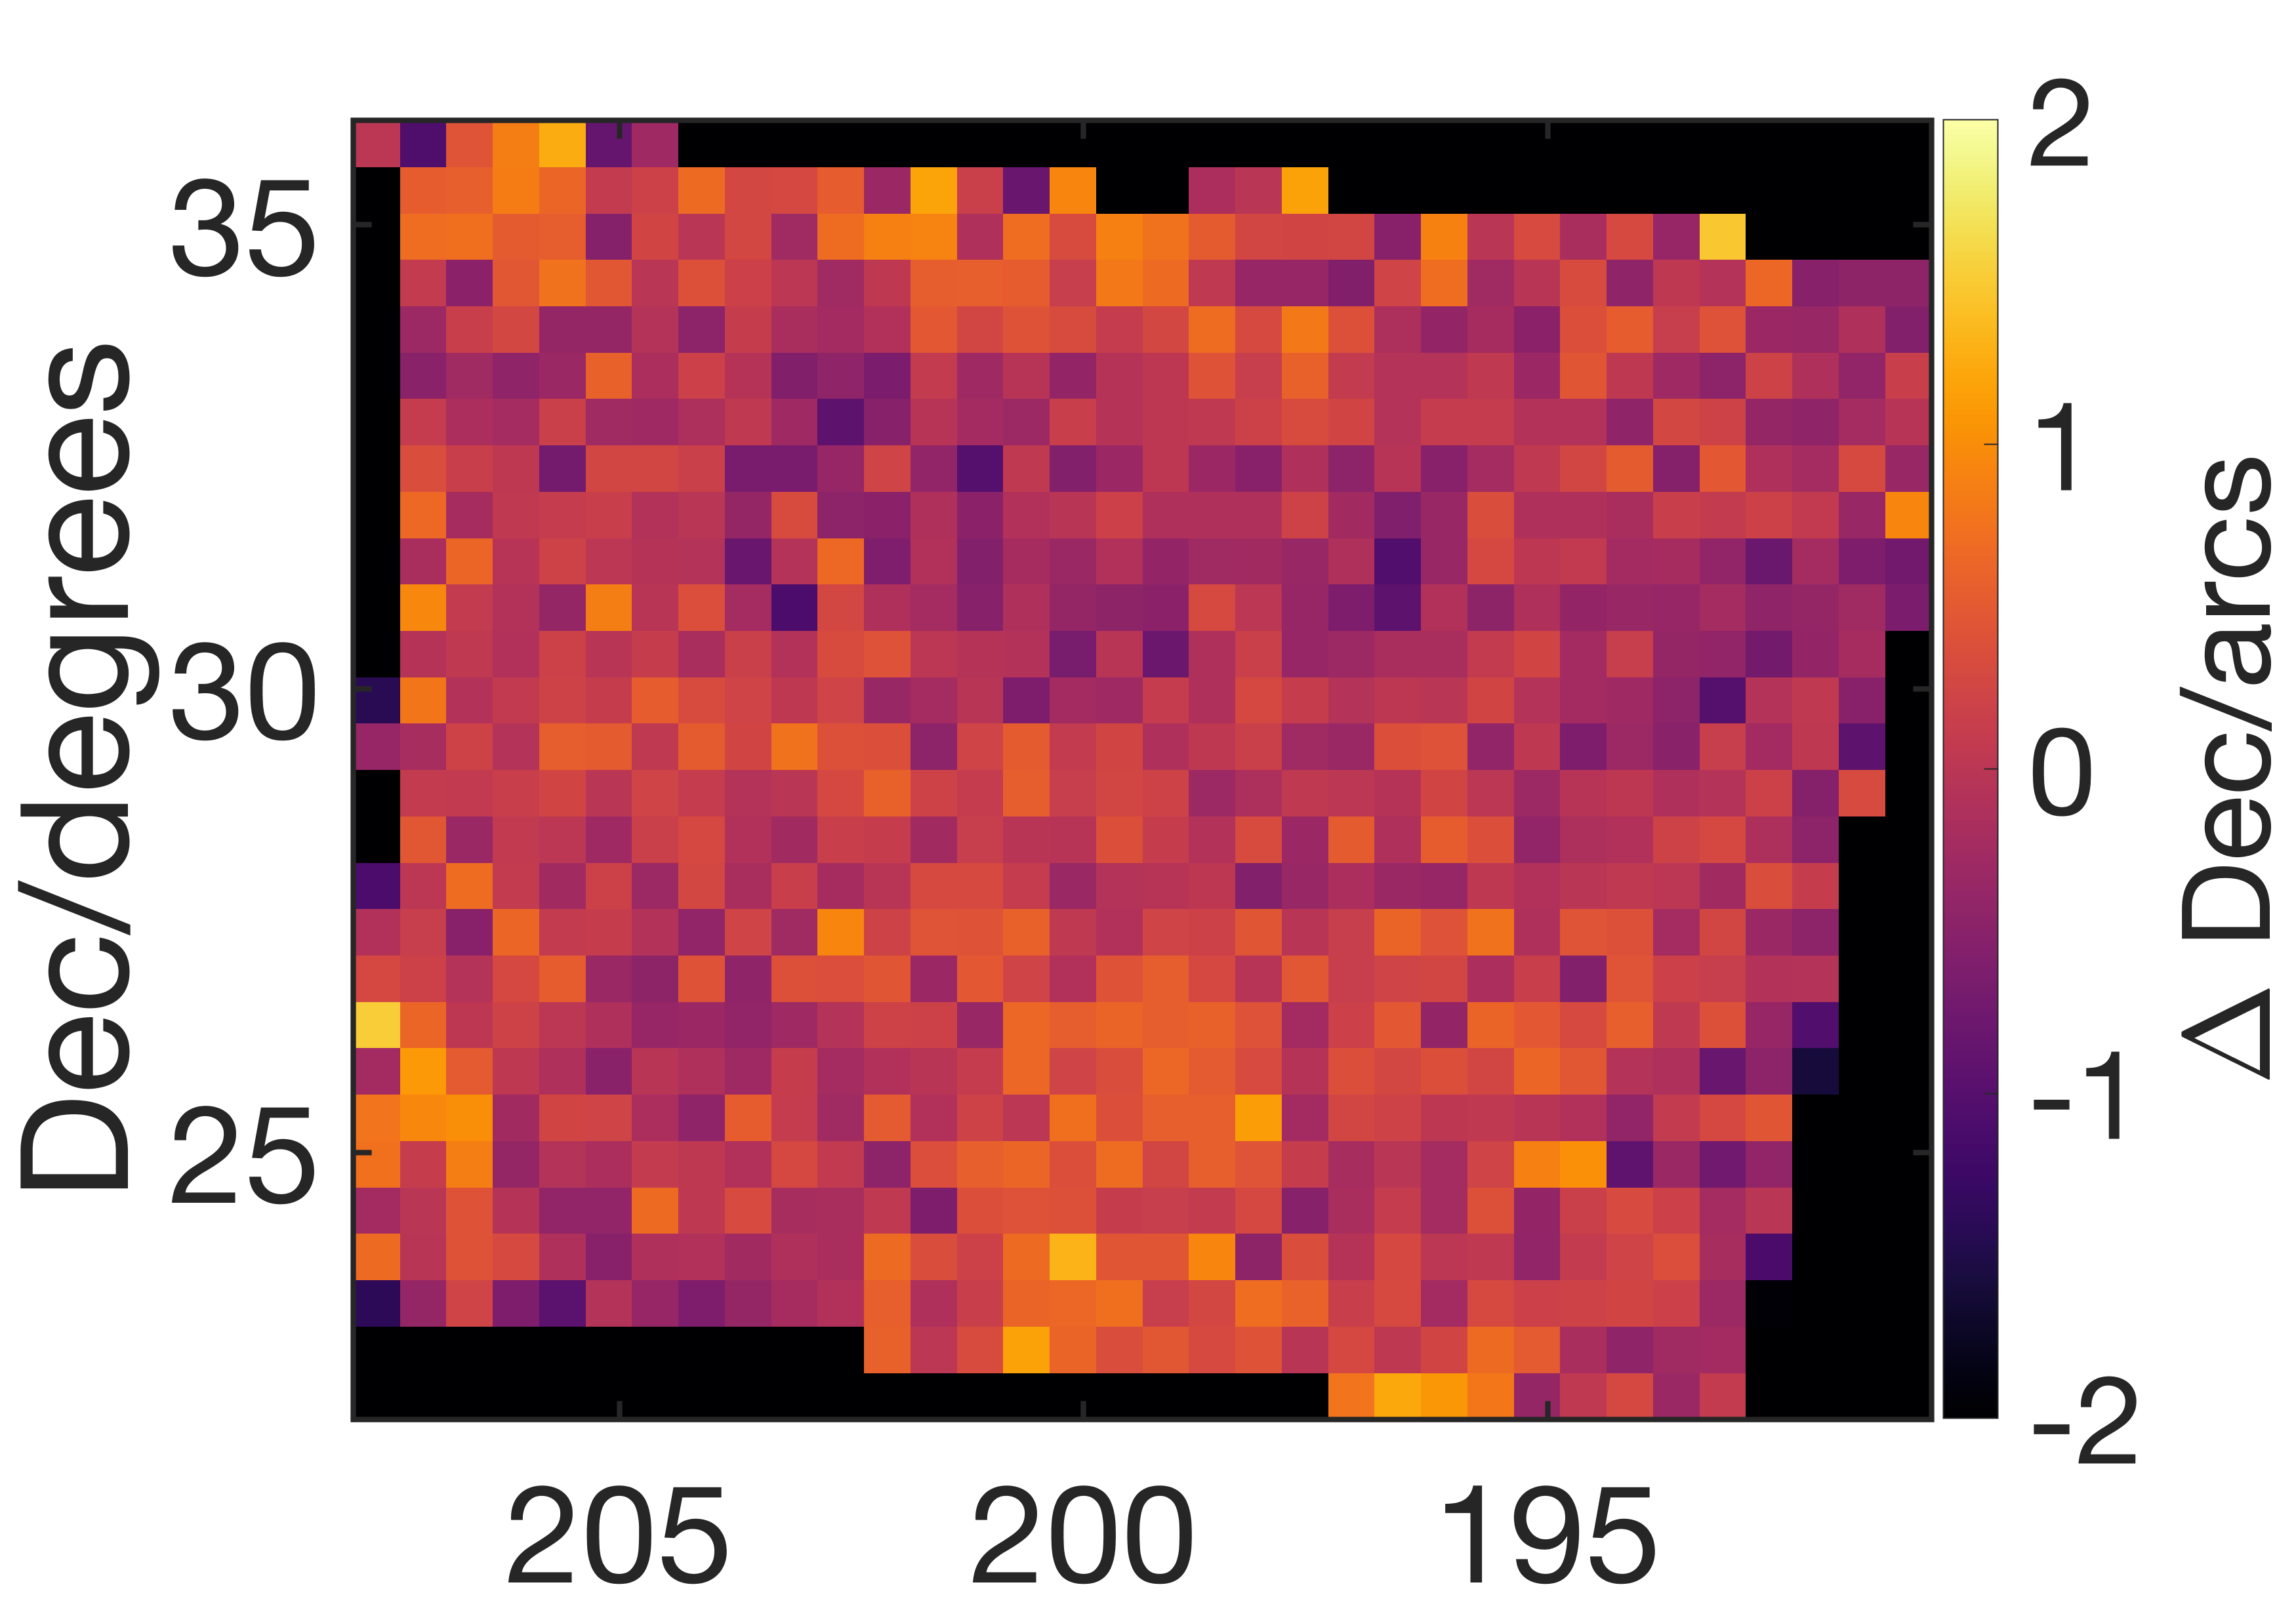
\includegraphics[scale=0.23]{ngp_ddec.png}
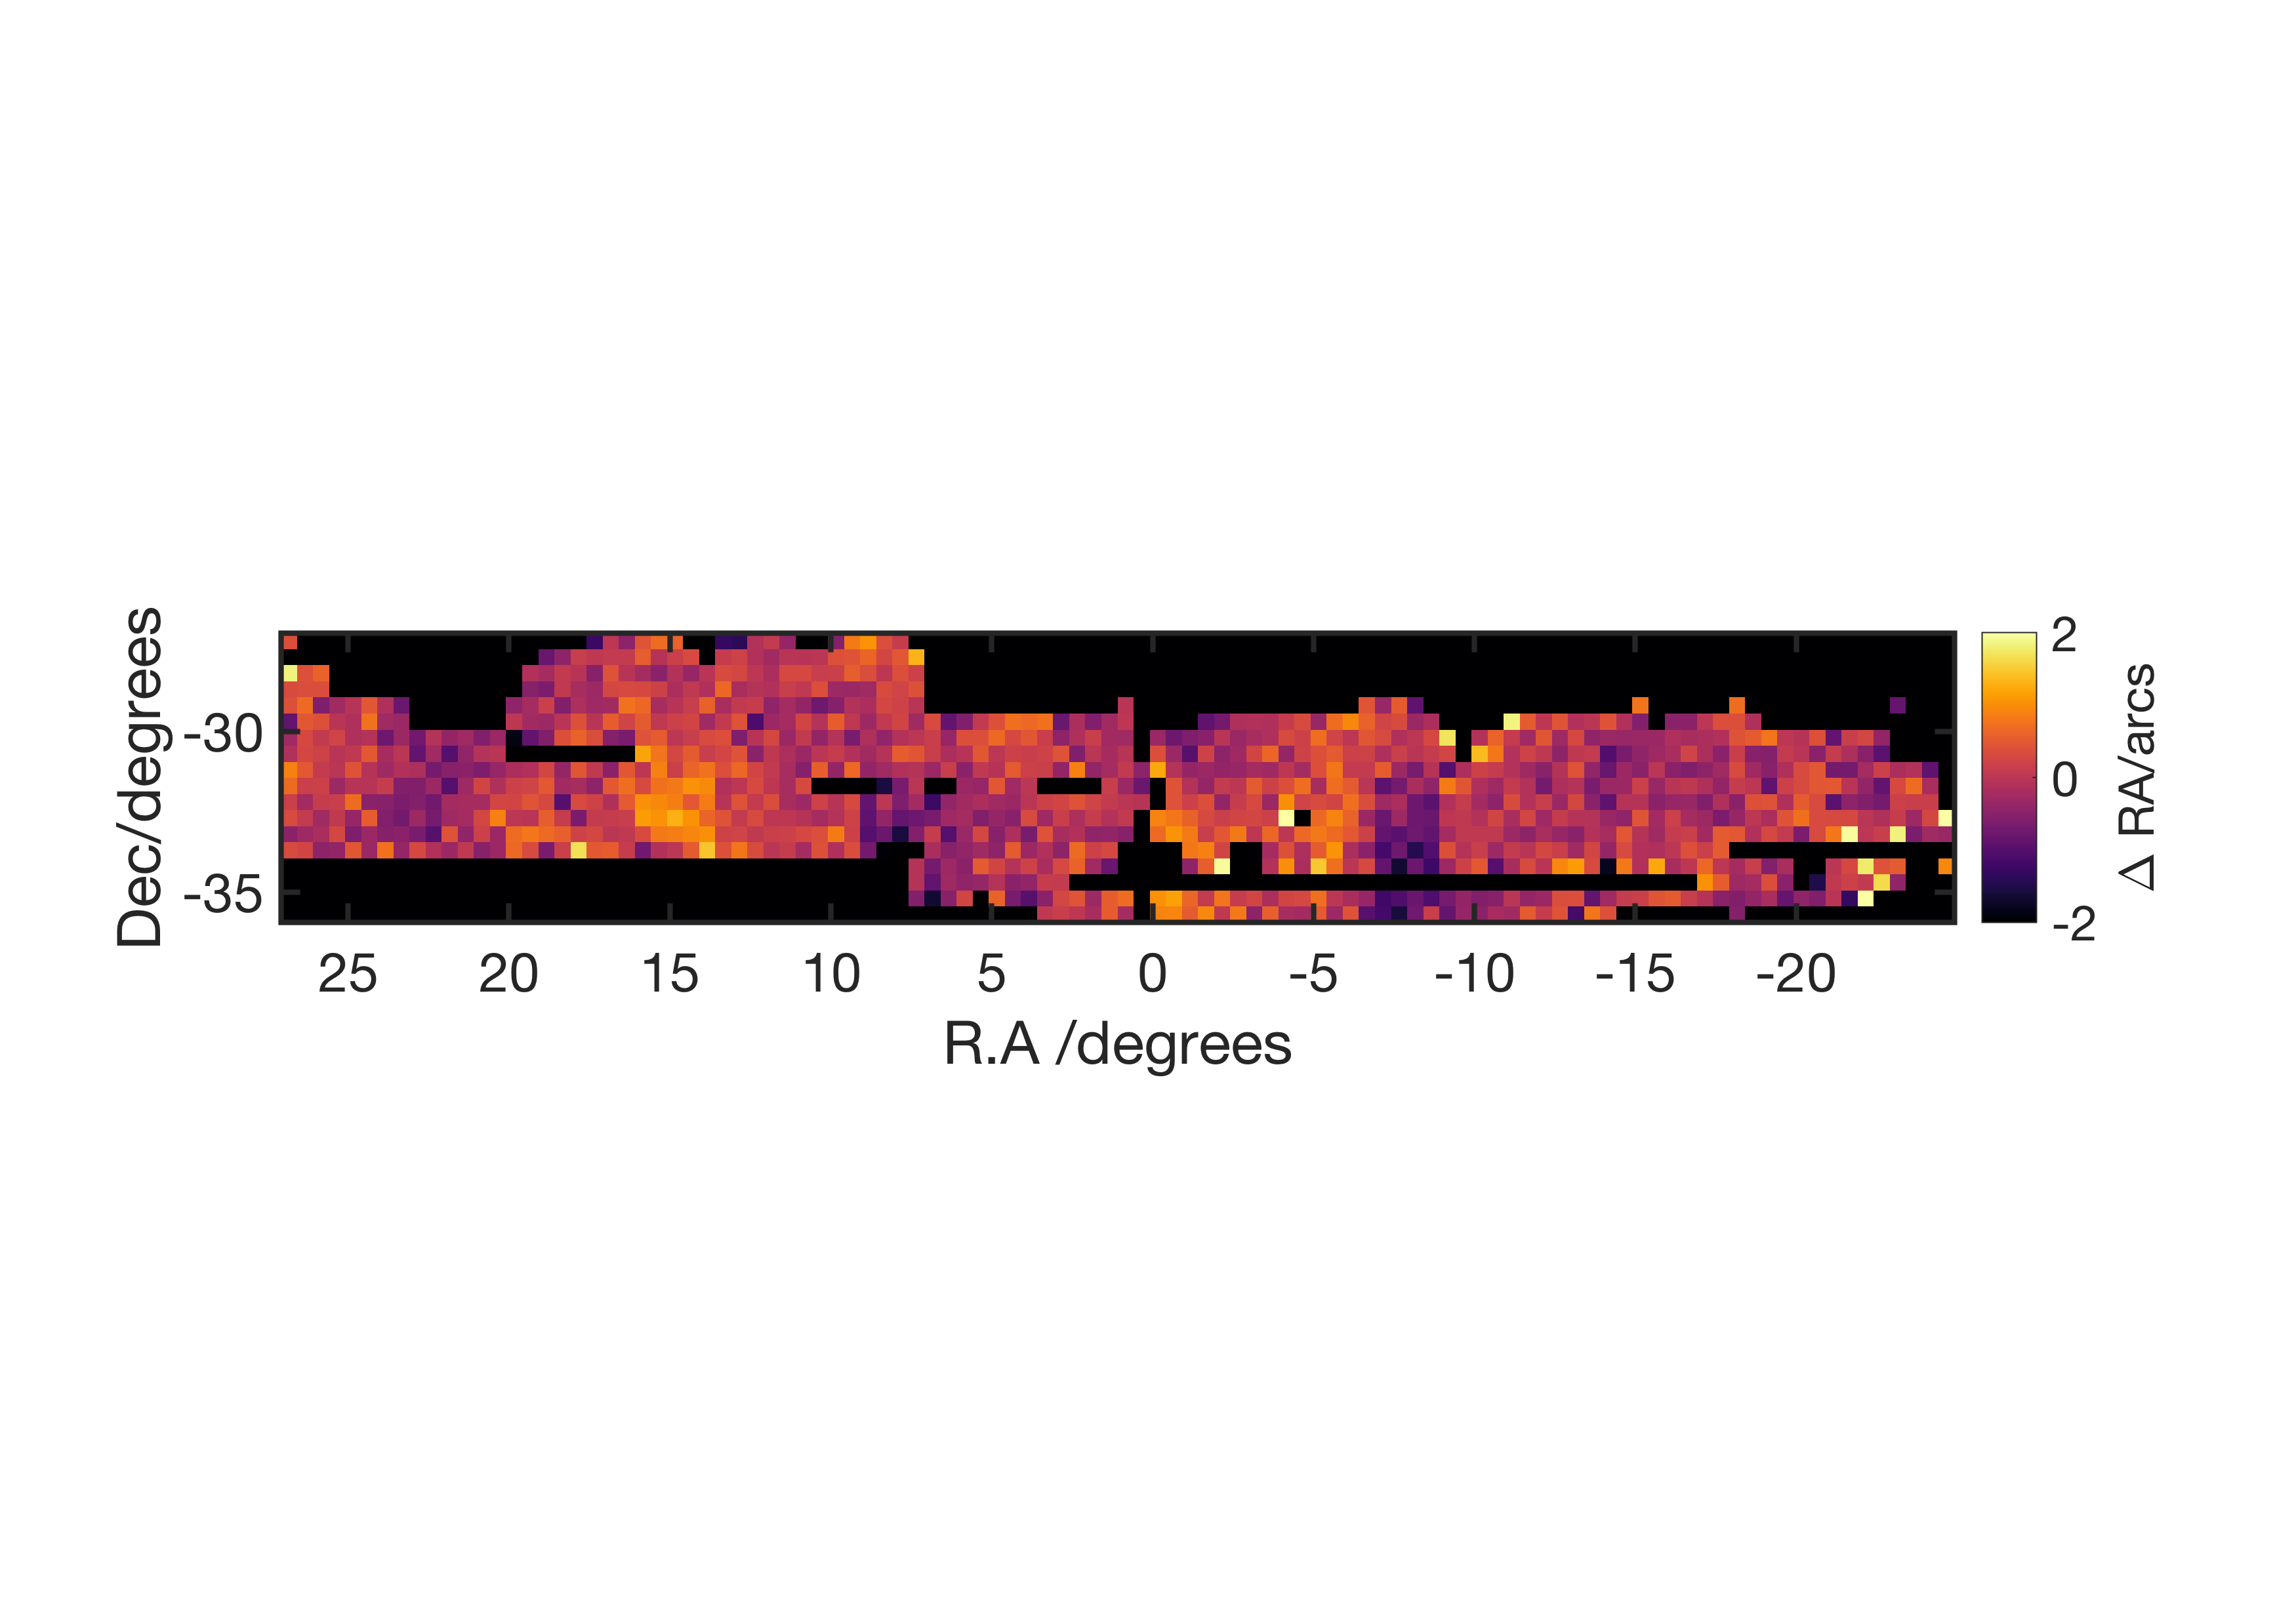
\includegraphics[scale=0.6,trim={0 87mm 0mm 75mm}, clip]{sgp_dra.png}
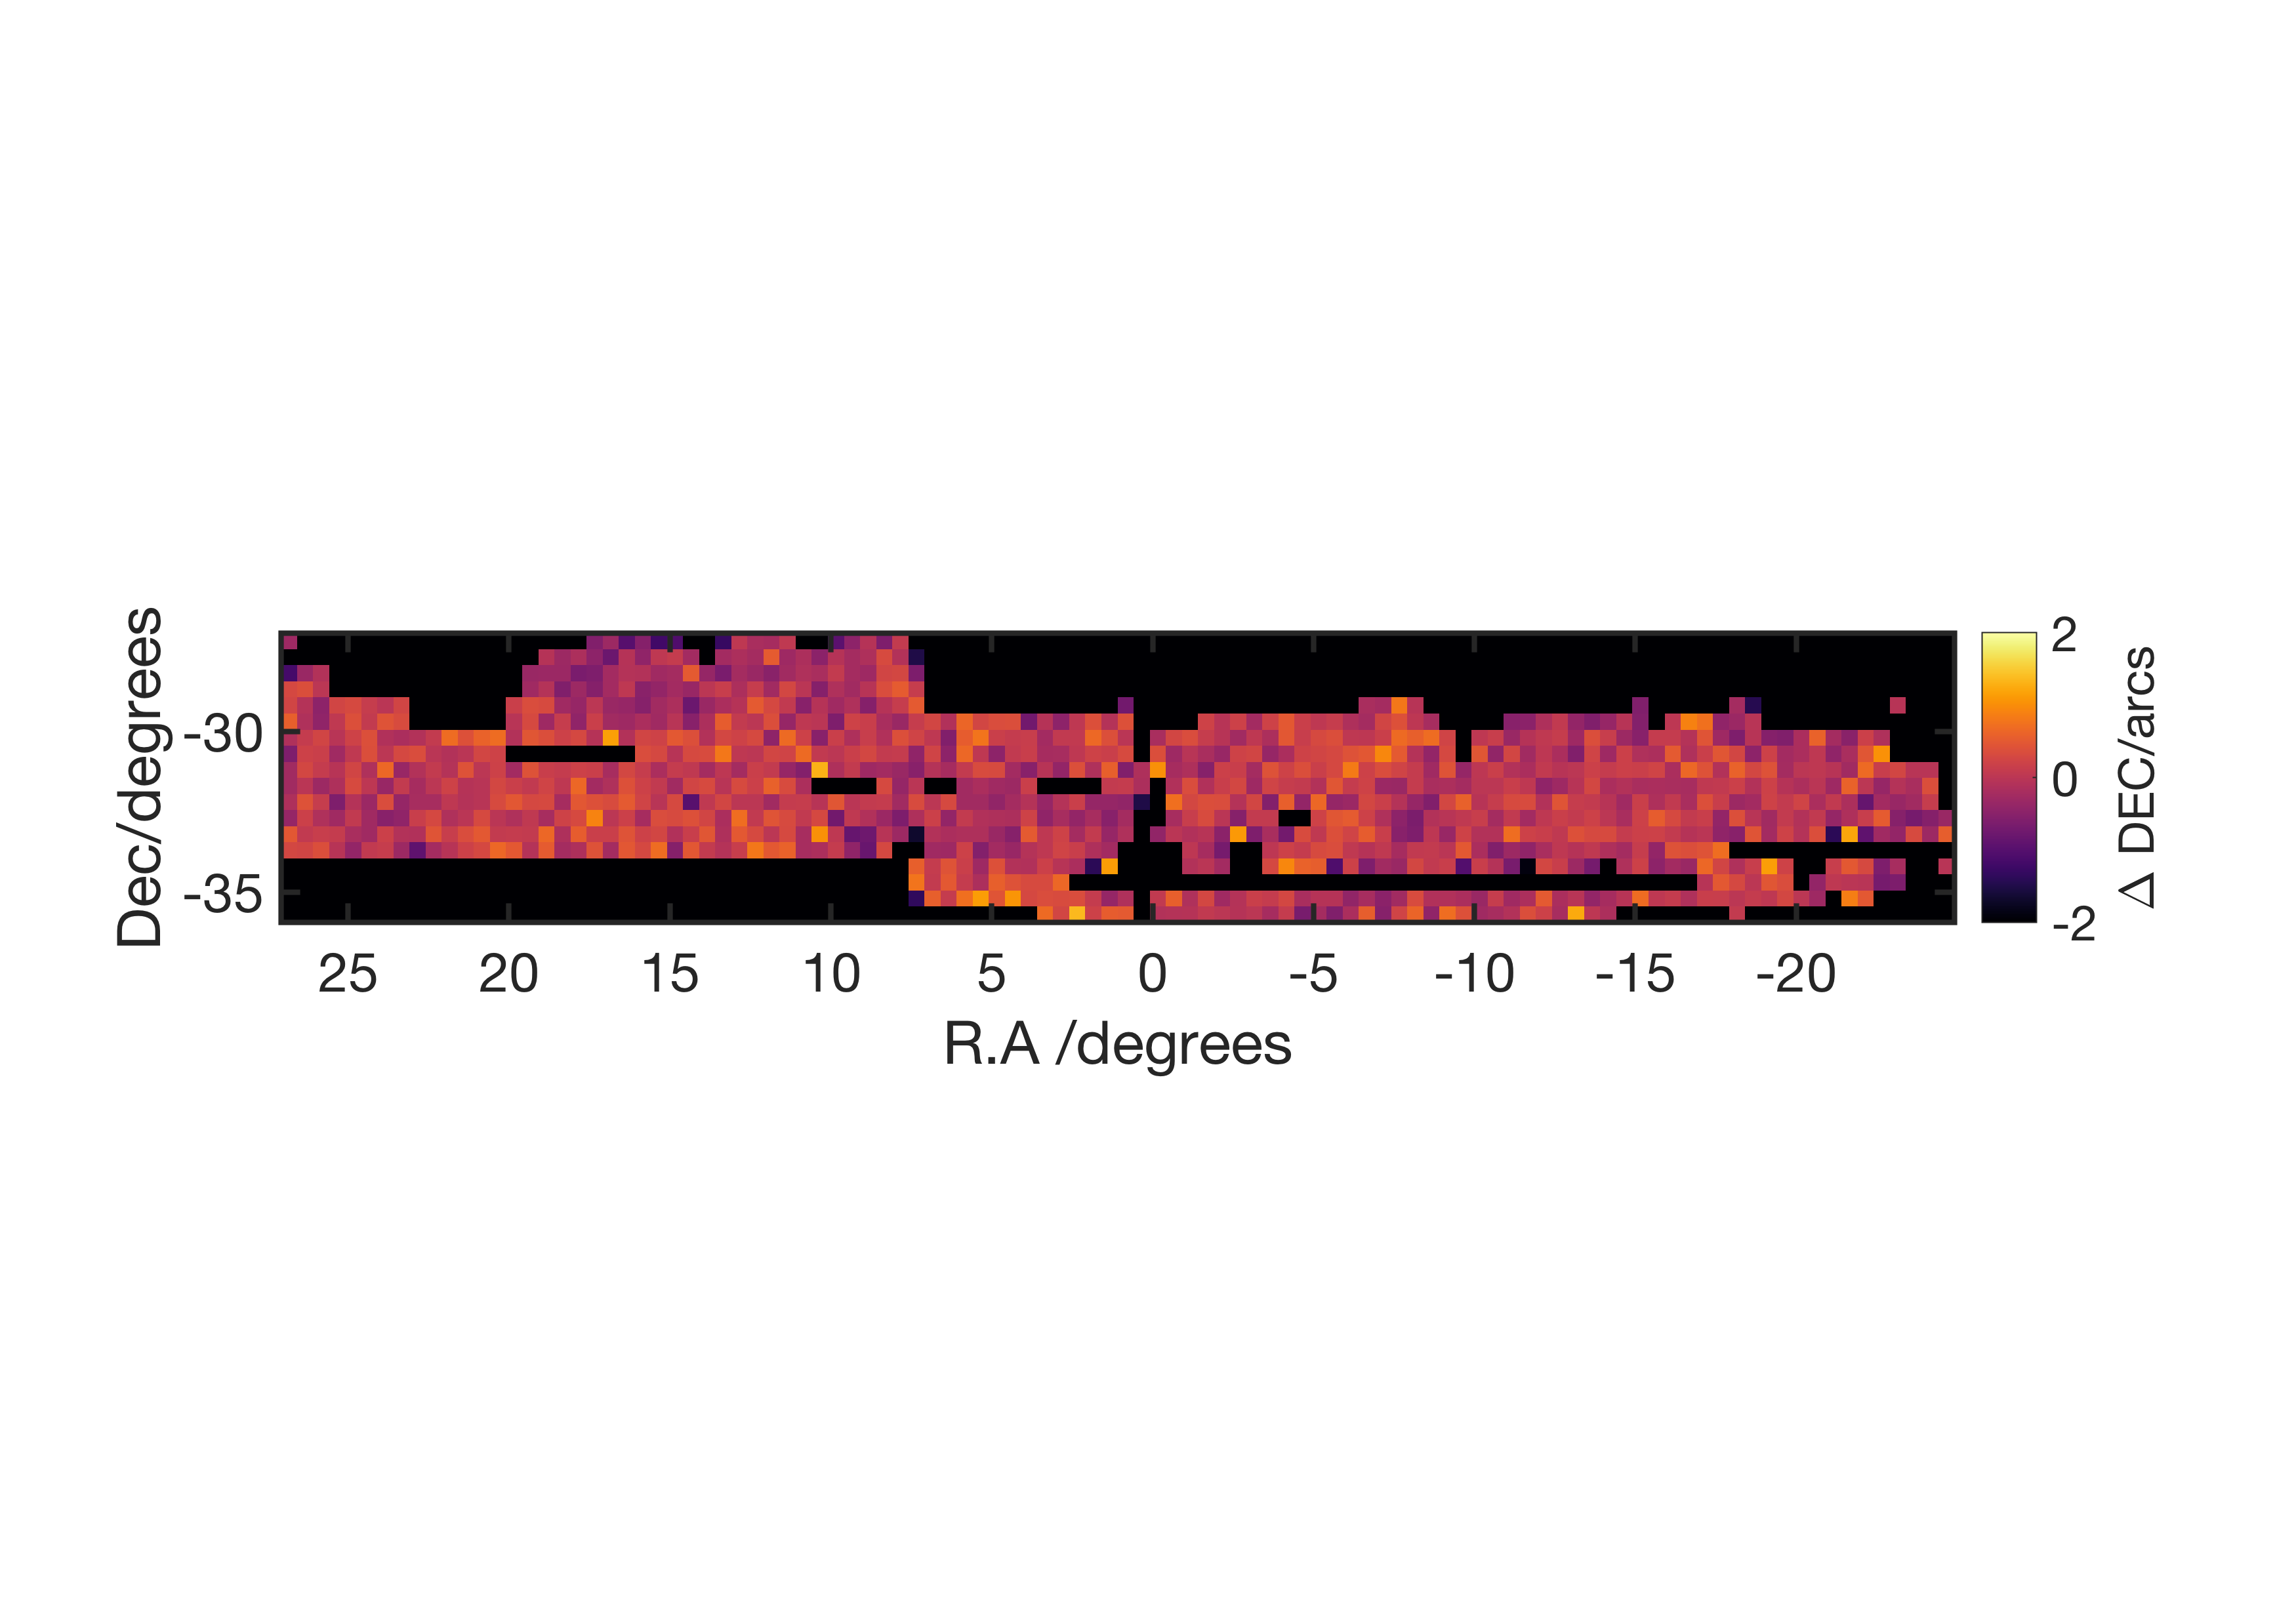
\includegraphics[scale=0.6,trim={0 60mm 0mm 80mm}, clip]{sgp_ddec.png}
\caption{\protect\label{fig_pos_errs} The mean positional errors in
  R.A and Dec. averaged in 0.5 degree areas as a
  function of position on the sky for the NGP field and the SGP
  fields. 
}
\end{figure*} 



\section{Completeness and Purity}

To estimate the efficiency of the source detection process we added
fake sources to the real maps and re-ran the source detection.  We
used several thousand sources with fluxes ranging from 6\ mJy to
300\ mJy, and find that the completeness of our 4$-\sigma$ sample is
about 90\%.  More the details of the simulations are described by V16.

The purity of the sample - ie the fraction of apparent sources that
correspond to real astronomical sources - is hard to estimate
reliably. Since the pixel histogram is highly skewed to positive
values, simply inverting the map and counting the number of negative
'sources' does not give a fair measure of the number of noise sources
that may be present in the real data. Most of these 'noise' sources will
be due to clumps of unresolved faint sources, and not instrumental
noise. With the 4$-\sigma$ cut, we expect the number of false
detections to be $\lesssim 0.5$\%. 


%\section{Colour Distribution} 
%
%Observed distribution of sources in SPIRE colour-colour space and
%comparison to simple modified black body spectra.  
%\begin{figure*}
%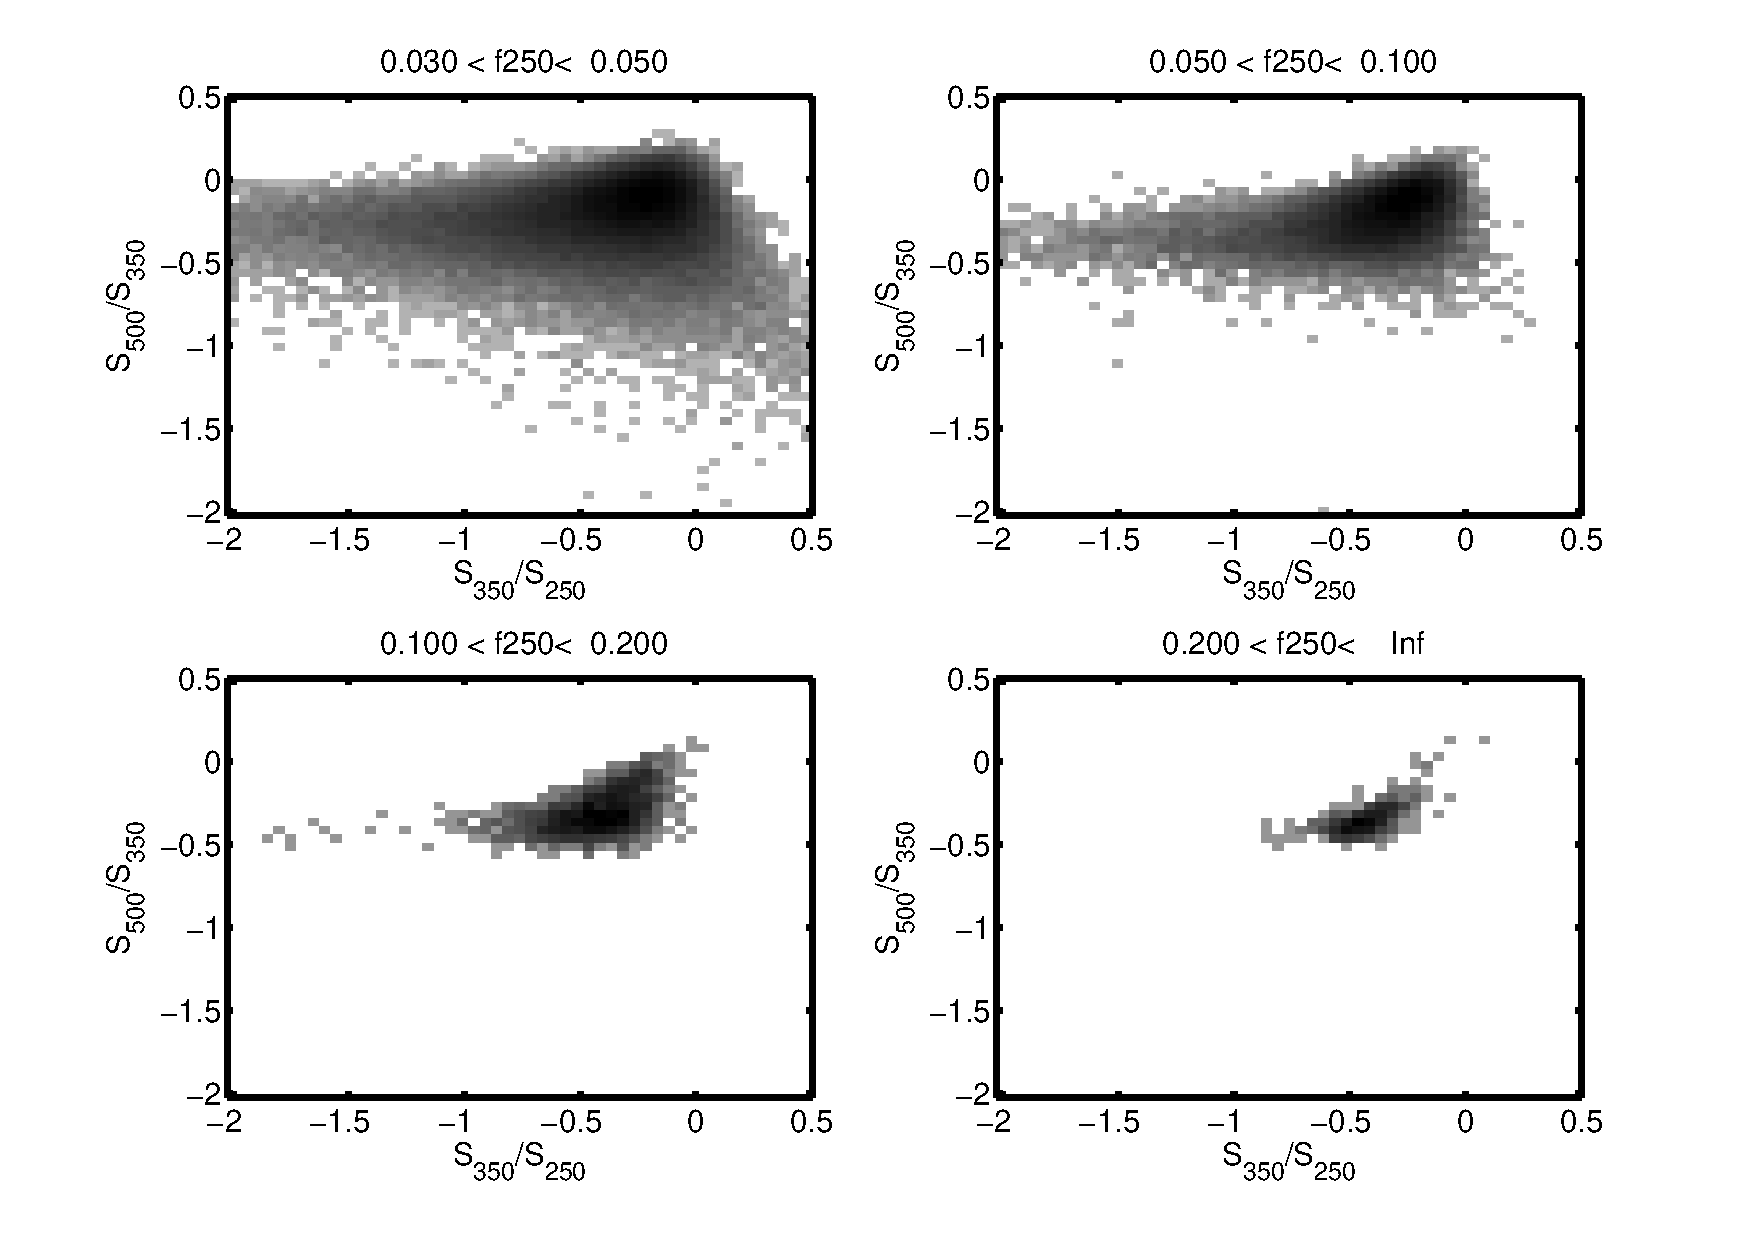
\includegraphics[scale=0.6]{NGP_col_plot.pdf}

%\caption{\protect\label{fig_colours} The distribution of sources as a
%  function of flux ratios $S_{350}/S_{250}$ and $S_{500}/S_{350}$ for
%  4 bins of 250\mic flux:  30~mJy$<S_{250}<$50~mJy ;
%  50~mJy$<S_{250}<$100~mJy ;  100~mJy$<S_{250}<$200~mJy ;  200~mJy$<S_{250}$ 
%flux. } 

%\end{figure*}



\section*{Acknowledgments}

LD and SJM acknowledge support from the ERC in the form of the
Advanced Investigator Program, COSMICISM (ERC-2012-ADG-20120216, PI
R.J.Ivison), and the Consolidator Grant, COSMIC DUST
(ERC-2014-CoG-647939, PI H.L.Gomez). 

\begin{thebibliography}{}

\bibitem[Bertin \& Arnouts(1996)]{sext} Bertin, E., \& Arnouts, S.\ 1996, \aaps, 117, 393 

\bibitem[Clements et al.(2010)]{clements} Clements, D.~L., et  al.\ 2010,  A\&A, in press, arXiv:1005.2409 

\bibitem[Driver et al. (2009)]{gama}Driver, S.P., et al., 2009,
  Astron. Geophys.,  50, 5.12

\bibitem[Dunne et al (2000)]{slugs} Dunne, L., Eales, S. A., Edmunds,
  M., Ivison, R., Alexander, P., \& Clements, D. L. 2000, MNRAS, 315,
  115

\bibitem[Dye et al. (2009)]{dye}Dye, S., et al., 2009 ApJ., 703, 285

\bibitem[Eales et al.(2010)]{eales} Eales, S., et al.\ 2010,  \pasp, 122, 499 

\bibitem[Griffin et al. (2010)]{spire} Griffin et al. 2010 A\&A this issue.

\bibitem[Ibar et al. (2010)]{pacsmaps} Ibar, E., 2010, MNRAS, submitted

\bibitem[Ivison et al.(2007)]{ivison} Ivison, R.~J., et al.\ 2007, \mnras, 380, 199 

\bibitem[Maddox et al.(2010)]{wtheta} Maddox, S.~J., et al.\  2010,  A\&A, in press, arXiv:1005.2406 

\bibitem[Negrello et al.(2007)]{negrello} Negrello, M., 
Perrotta, F., Gonz{\'a}lez-Nuevo, J., Silva, L., de Zotti, G., Granato, 
G.~L., Baccigalupi, C., \& Danese, L.\ 2007, \mnras, 377, 1557 

\bibitem[Ott et al. (2010)]{hipe} Ott, S. 2010, in ASP Conference Series, Astronomical Data Analysis 
Software and Systems XIX, Y. Mizumoto, K.-I. Morita, and M. Ohishi, eds., in press 

\bibitem[Pascale et al. (2010)]{spiremaps}Pascale, E., et al, 2010, MNRAS, submitted

\bibitem[\protect\citeauthoryear{{Pilbratt}}{{Pilbratt et al.}}{2010}]{herschel} Pilbratt, G.~L., et al. A\&A in press, arXiv:1005.5331 

\bibitem[Poglitsch et al. (2010)]{pacs} Poglitsch, A., et al. 2010 A\&A, in press, arXiv:1005.1487 

\bibitem[Rigby et al. (in prep)]{rigby} Rigby, E.E, et al., MNRAS. 

\bibitem[Rowan-Robinson (2001)]{rr} Rowan-Robinson, M. 2001, in IAU
  Symp. 204, The Extragalactic Infrared Background and its
  Cosmological Implications, ed. M. Harwit \& M. G.  Hauser (Dordrecht:
  Kluwer), 265


\bibitem[Schlegel et al.(1998)]{iras_ref} Schlegel, D.~J., 
Finkbeiner, D.~P., \& Davis, M.\ 1998, \apj, 500, 525 

\bibitem[Smith et al. (2010)]{Smith} Smith, D et al, 2010,  MNRAS, in prep

\bibitem[Wang \& Rowan-Robinson(2009)]{iras} Wang, L., \& Rowan-Robinson, M.\ 2009, \mnras, 398, 109 

\end{thebibliography}
\section{Appendix}

The catalogue files are available from {\tt
  http://www.h-atlas.org}. The columns and a short description each
parameter in the catalogue
and contain the following columns. 


\label{lastpage}

\end{document}

